\documentclass[10pt]{article}
\usepackage[margin=1in]{geometry}
\usepackage[utf8]{inputenc}
\usepackage{multicol}
\setlength{\columnsep}{1mm}
\usepackage{amsfonts}
\usepackage{booktabs}
\usepackage{siunitx}
\usepackage[authoryear,round]{natbib}
\usepackage{float}
\usepackage[font={small}]{caption}
\usepackage[labelfont=bf]{caption}
\usepackage{lineno}
\usepackage{amsmath,amssymb,setspace,fancyhdr,geometry,url,color}
\usepackage{subfigure,graphicx,caption}
\usepackage{lscape,amsthm}
\usepackage{blindtext}
\usepackage{hhline}
\usepackage{arydshln}
\usepackage{verbatim}
\usepackage{dblfloatfix}
\usepackage{multirow}
\usepackage{graphicx}
\usepackage{xr}
\externaldocument{../PhaseIIPaper/main}
%\biboptions{authoryear, comma}
%%%%%%%%%%%%%%%%%%%%%%%%%%%%%%%%%%%%%%%%%%%%%%%%%%%%%%%%%%%%%%%%%%%%%%%%%
%%%%%%%%%%%%%%%%%%%%%%%%%%%%%%%%%%%%%%%%%%%%%%%%%%%%%%%%%%%%%%%%%%%%%%%%%%
\begin{document}
\centering{\bf {\large Supplemental Material} \\
{\Large The GGCMI phase II emulators: global gridded crop model responses to changes in CO$_2$, temperature, water, and nitrogen (version 1.0)}}\\

\vspace{3mm}

\centering{James Franke$^{1}$, et al.
~\\}

\centering{
{\small 1.  Department of the Geophysical Sciences, University of Chicago, Chicago, IL, USA}\\
}

%\tableofcontents

%%%%%%%%%%%%%%%%%%%%%%%%%%%%%%%%%%%
\clearpage
%%%%%%%%%%%%%%%%%%%%%%%%%%%%%%%%%%%

\renewcommand{\thefigure}{S\arabic{figure}}

\section{Cultivation Areas}
\begin{figure}[h!]
\centering
%S1
\begin{minipage}{.45\textwidth}
    \centering
    \vspace{0pt}
    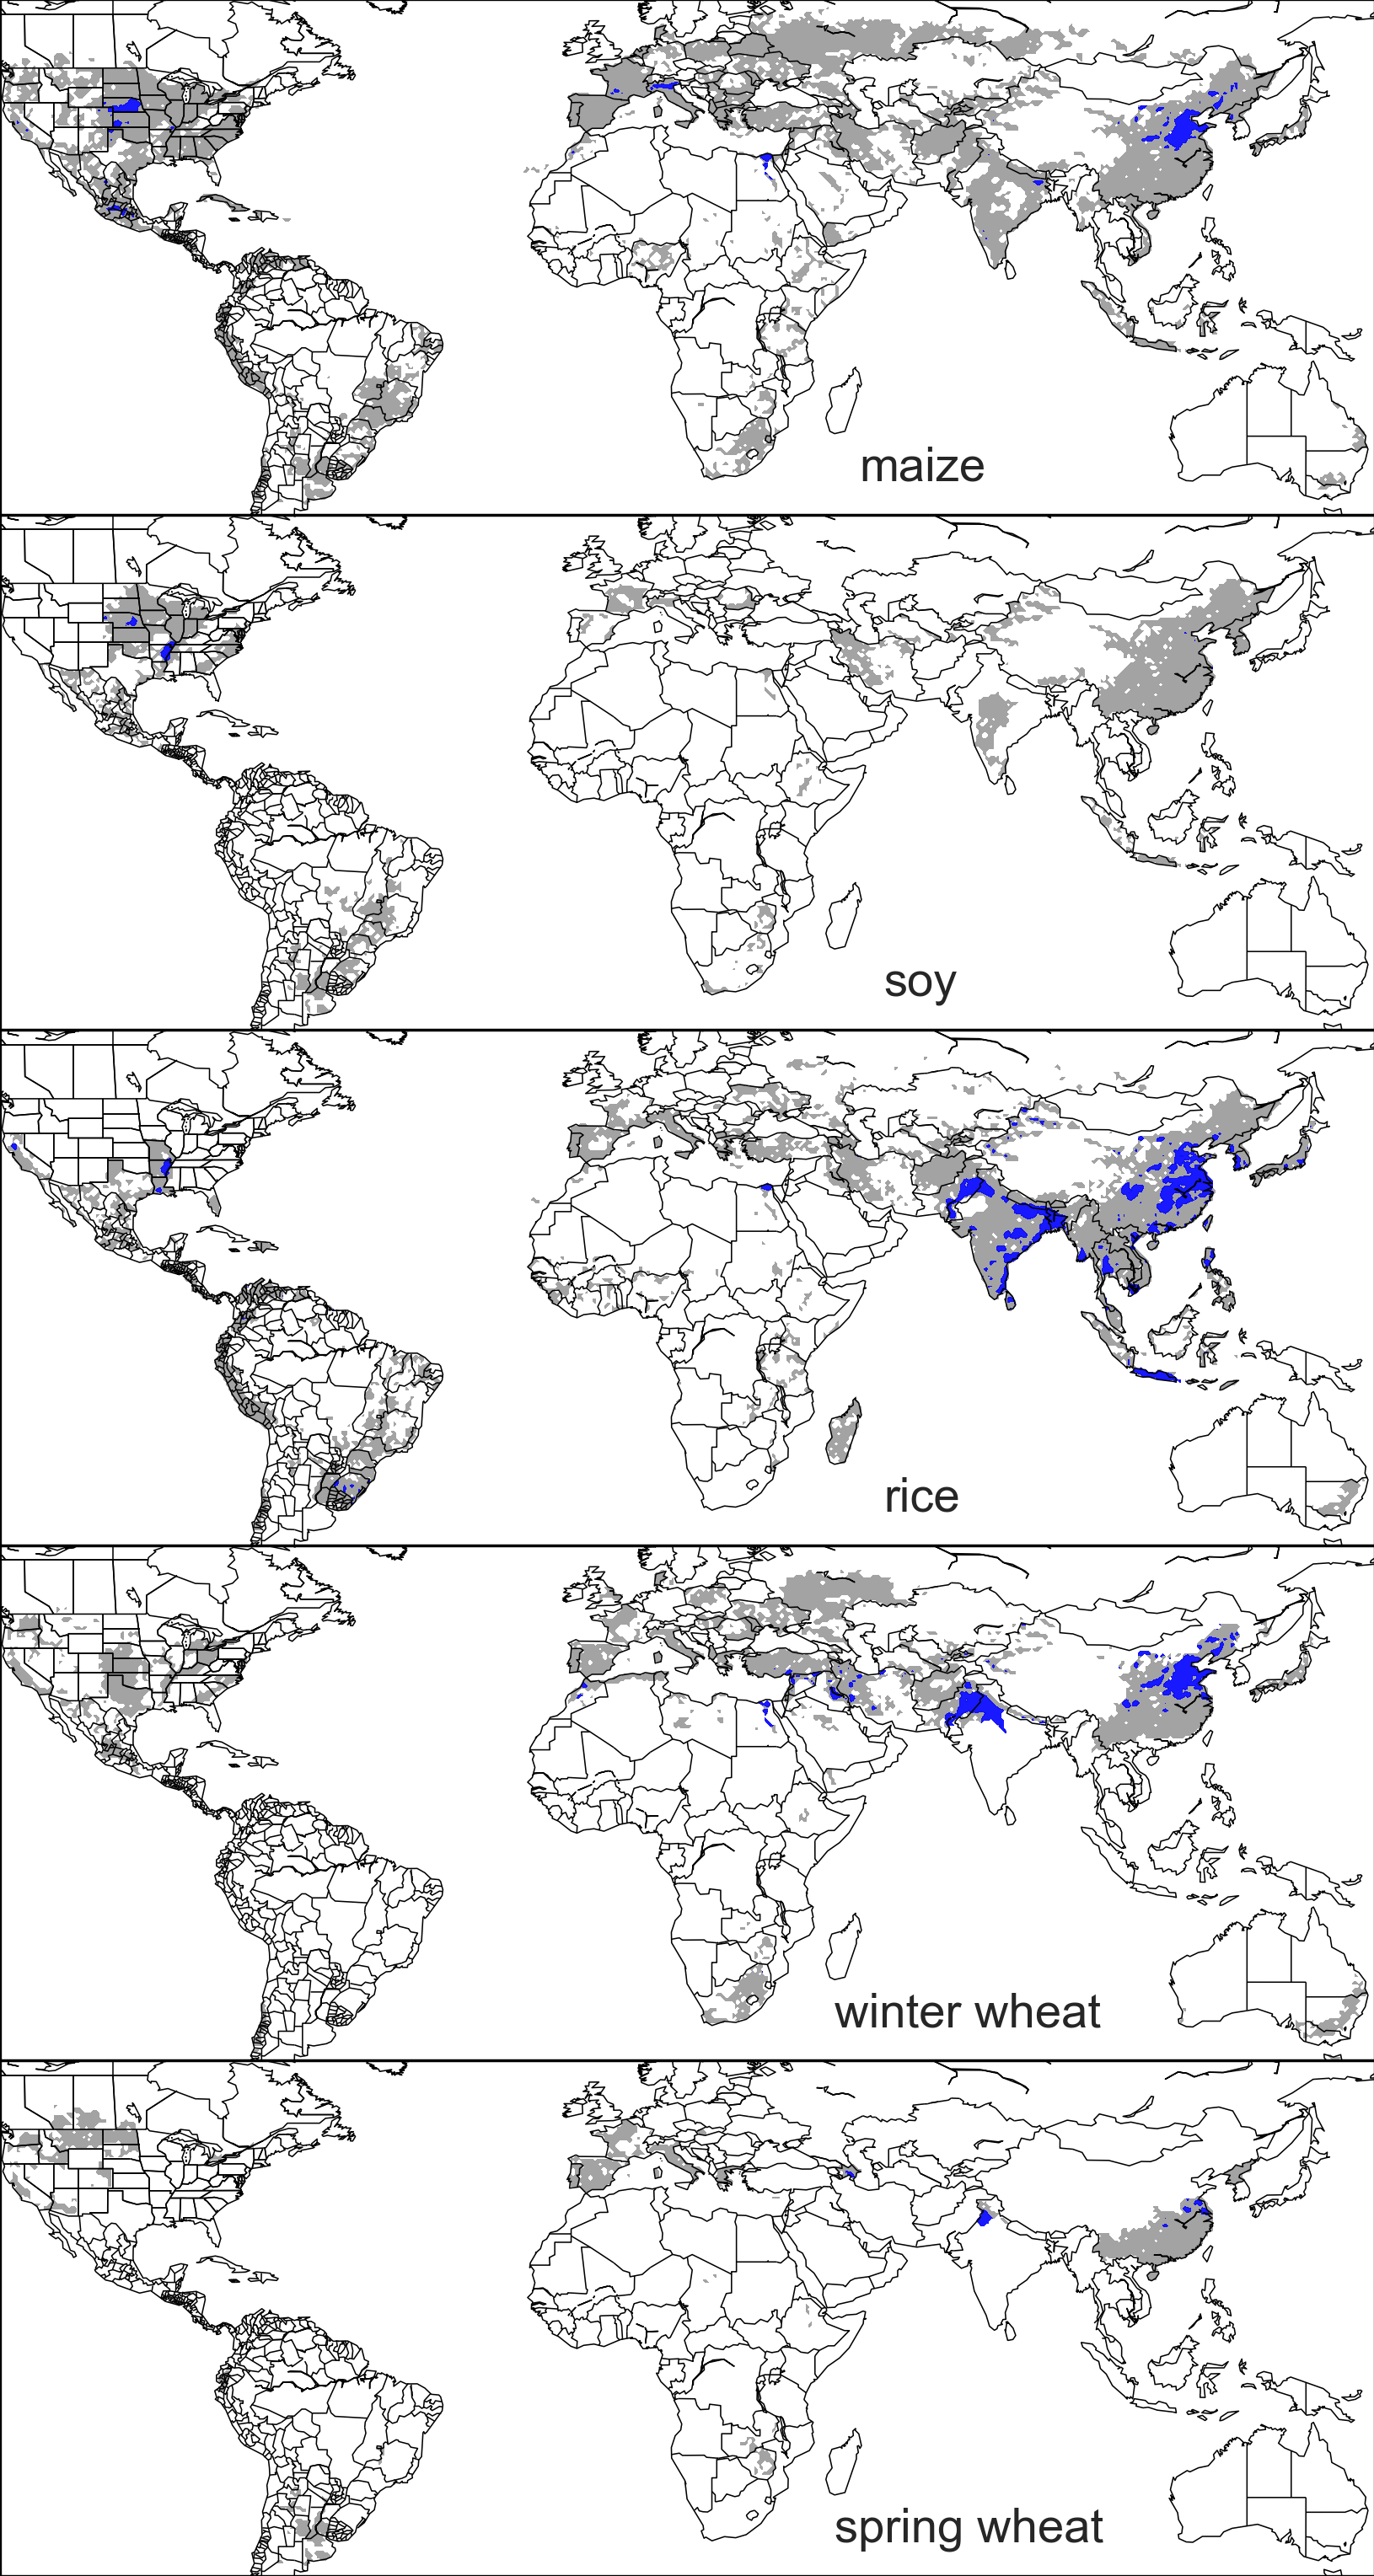
\includegraphics[width=\textwidth]{s_croparea_irr.png}\\
    \caption{Presently cultivated area for irrigated crops in the real world. The blue contour area indicates grid-cells with more that 20,00 hectares of crop cultivated. The gray contour shows area with more that 10 hectares cultivated. Data from the MIRCA2000 data set for maize, rice, and soy. Winter and spring wheat areas are adapted from MIRCA2000 data and sorted by growing season.}
    \label{fig:irrarea}
\end{minipage}
\hspace{.05\linewidth}
%S2
\begin{minipage}{.45\textwidth}
    \centering
    \vspace{-19mm}
    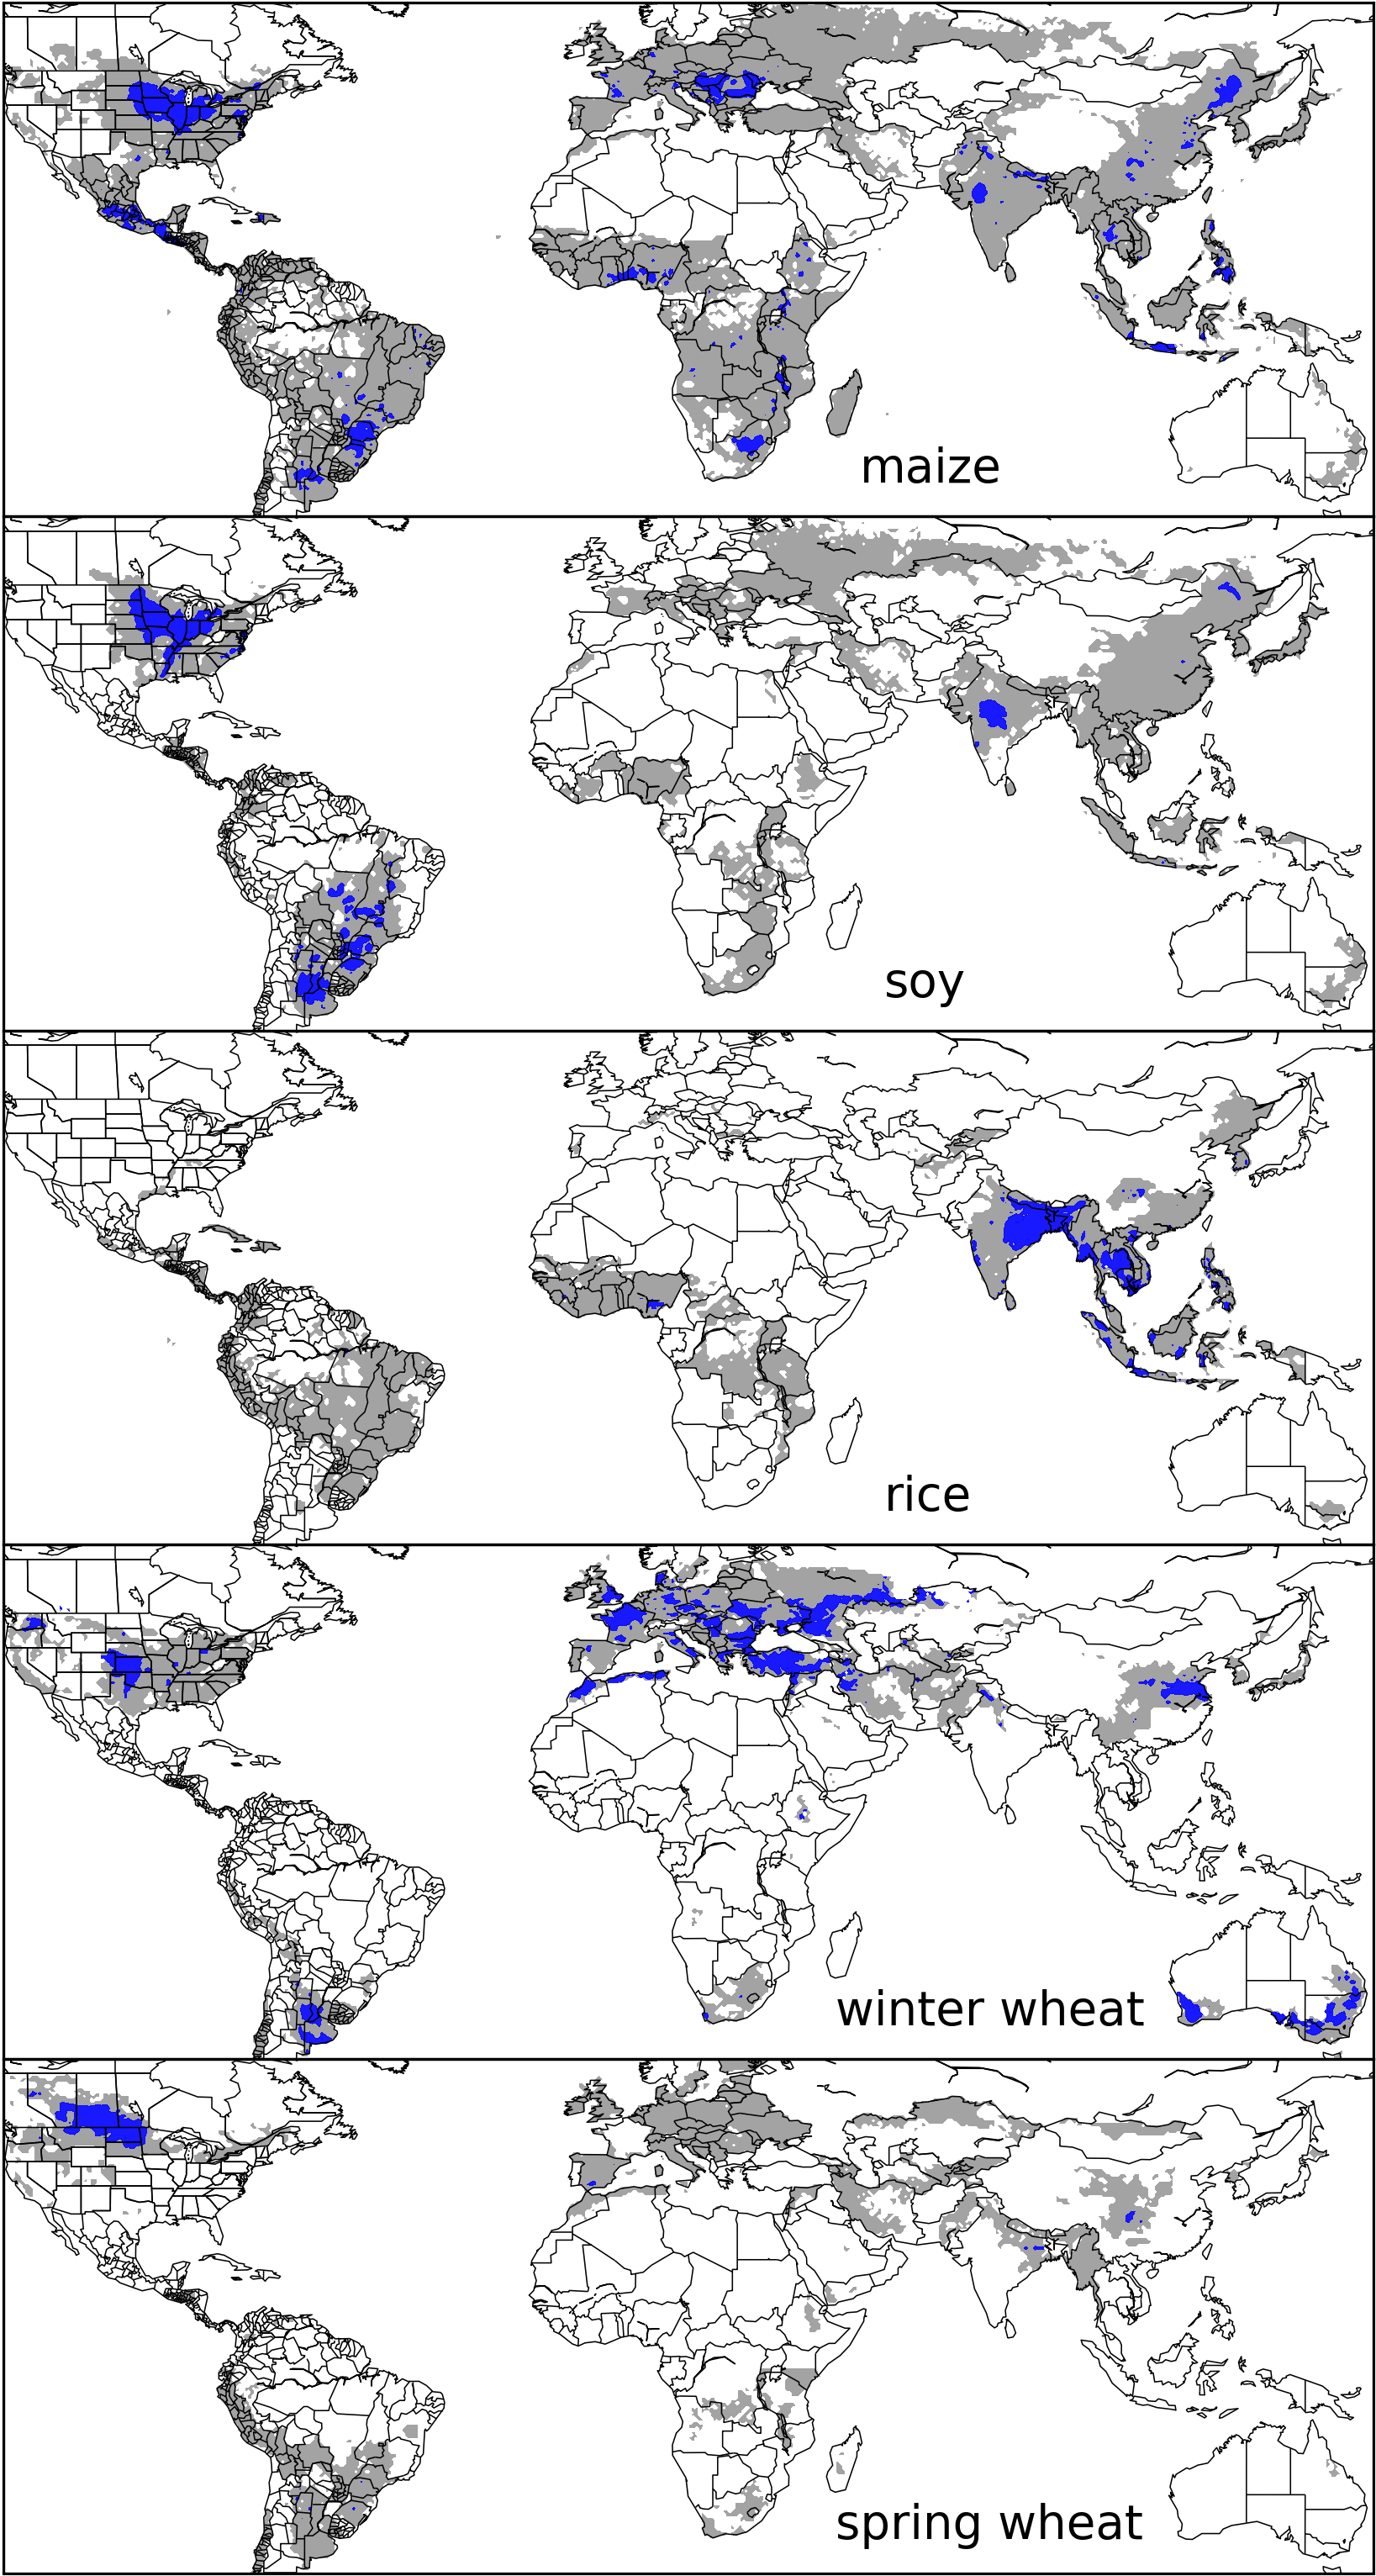
\includegraphics[width=\textwidth]{s_croparea.png}\\
    \caption{Presently cultivated area for rain fed crops in the real world. Conventions as in Figure S1.}
    \label{fig:rainfed}
\end{minipage}
\end{figure}

\clearpage
\section{Experiment Simulation Sampling in Variable Space}
\begin{figure}[h!]
%S3
\centering
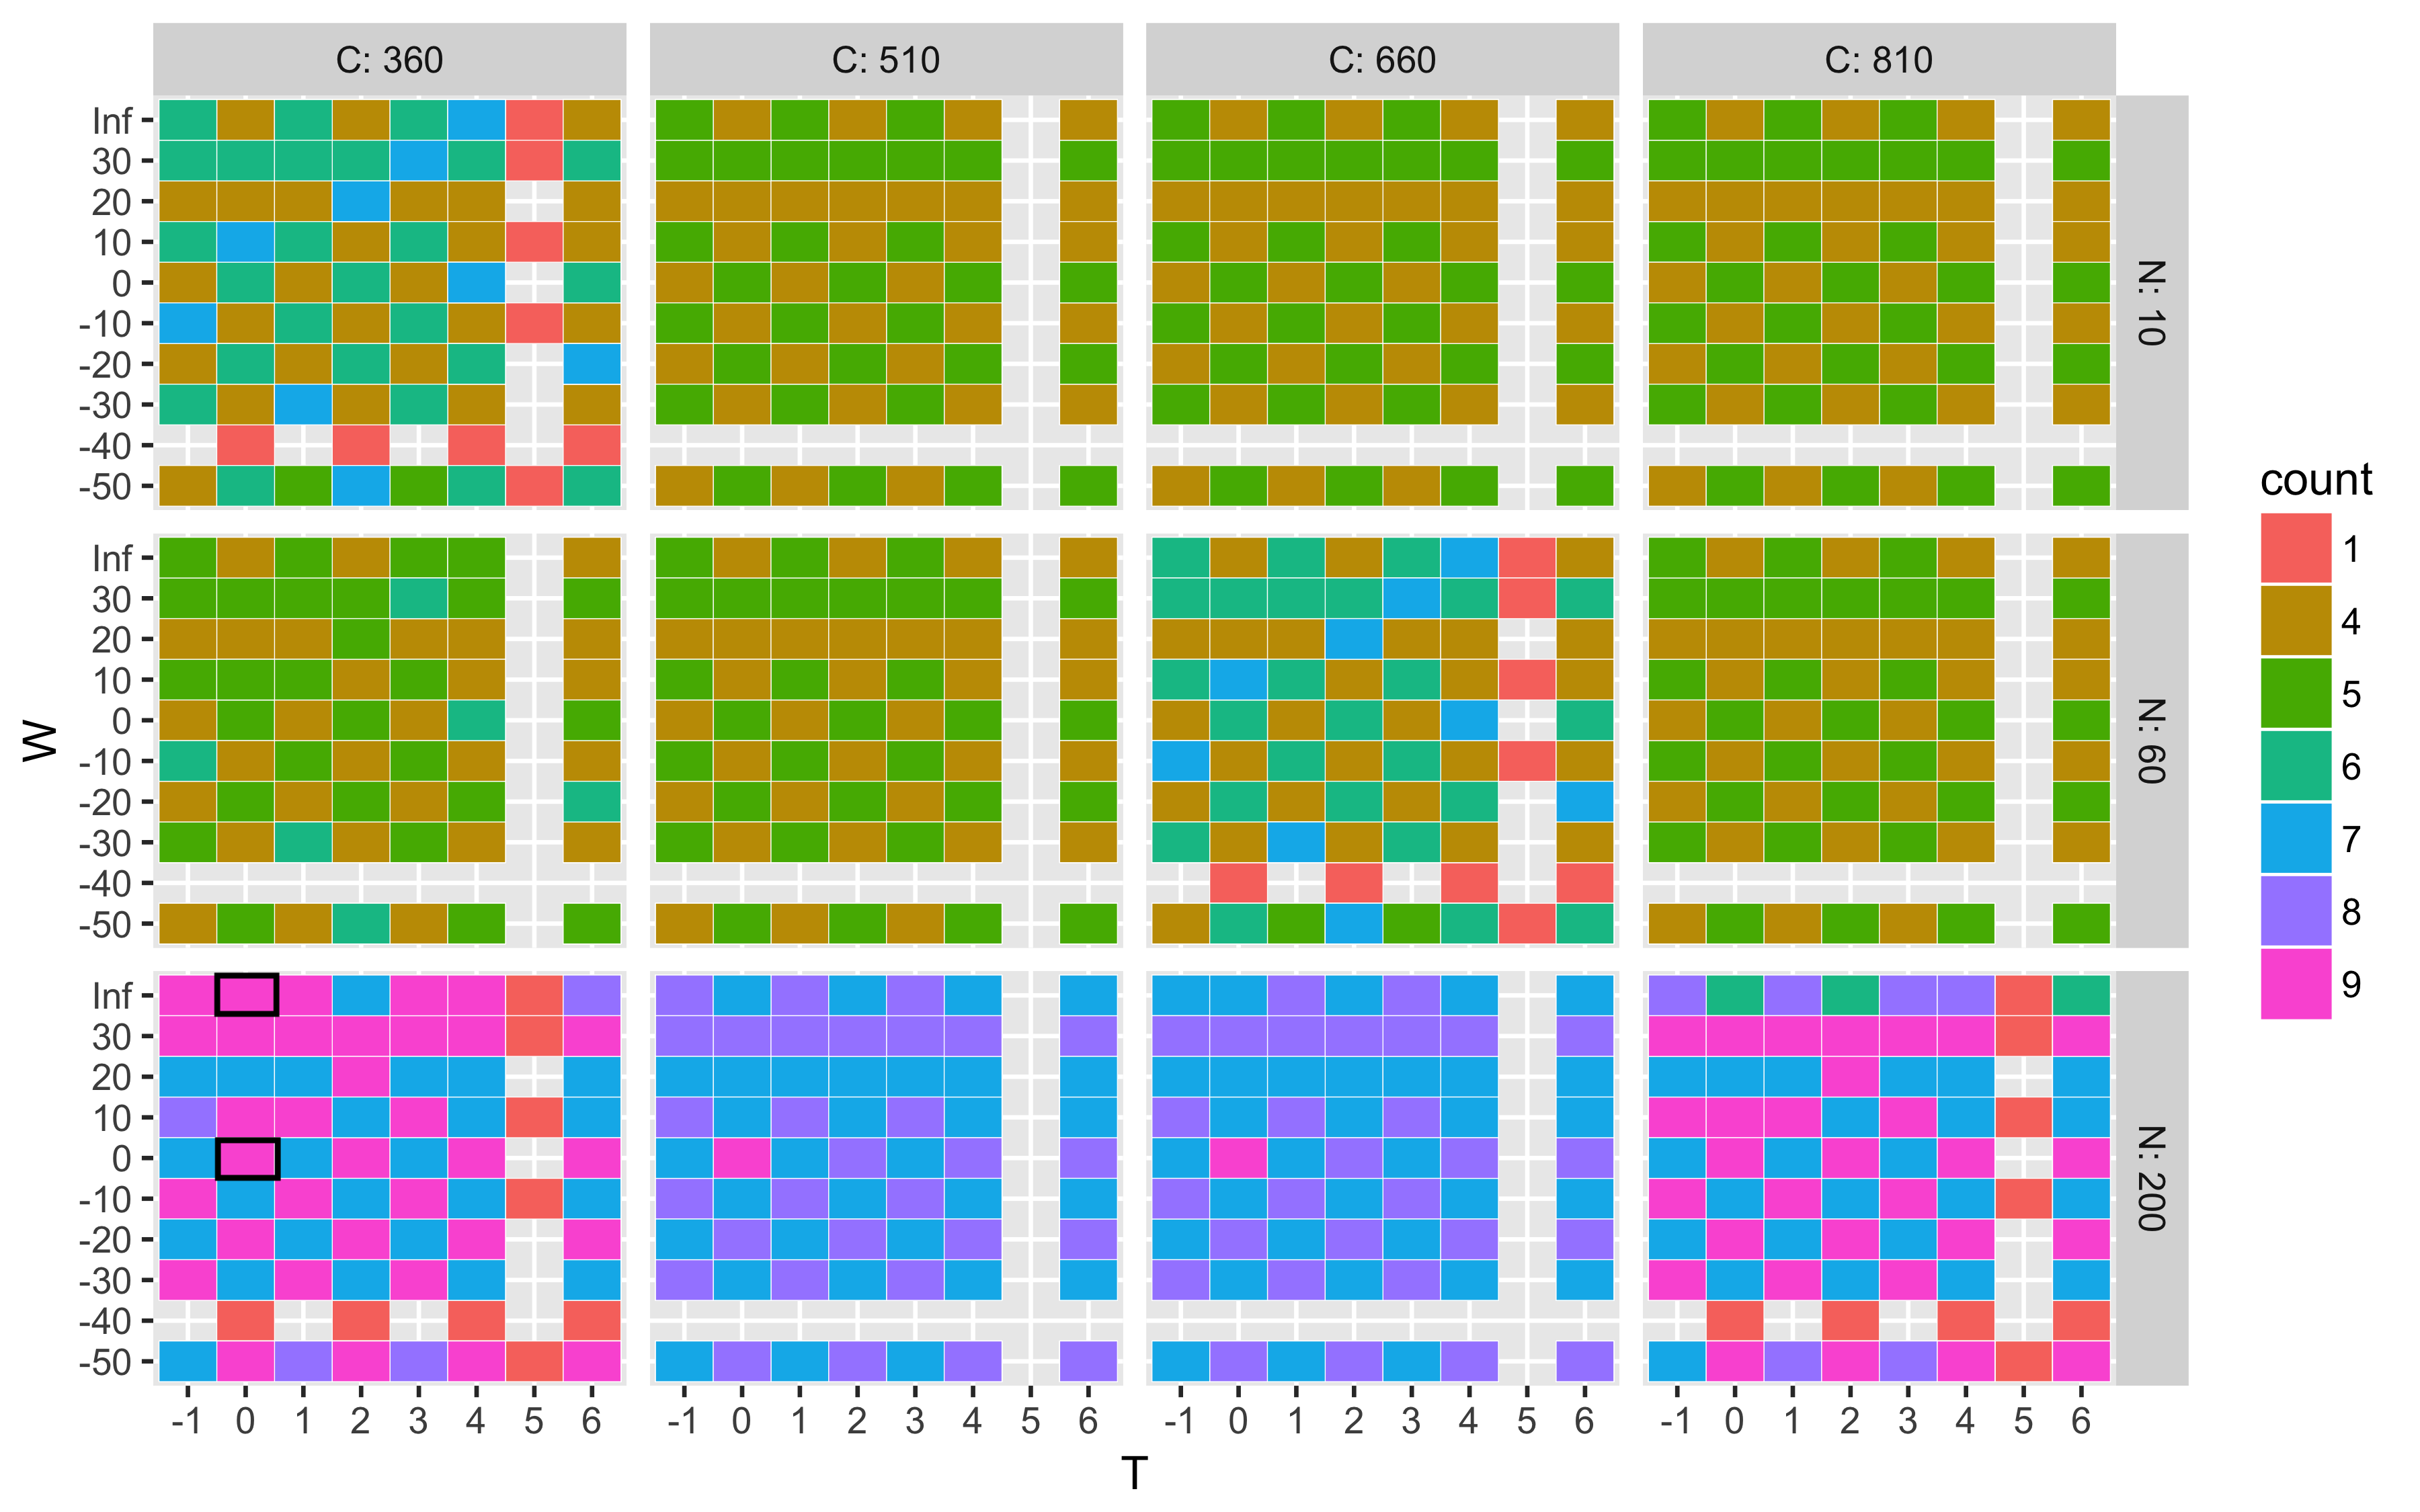
\includegraphics[width=\textwidth]{s_how_many_simulations.png}
\caption{Tile heatmap illustrates number of model simulations provided for each of the scenarios in the variable space. The max number is 9, the number of models included in the emulator analysis (excluding three models not included in the emulator analysis). Normalized rrror calculations are run over scenarios with max number of models.}
\label{fig:numbersims}
\end{figure}

\clearpage
\subsection{Year-to-year vs climatological mean}
\begin{figure}[h!]
%S4
\centering
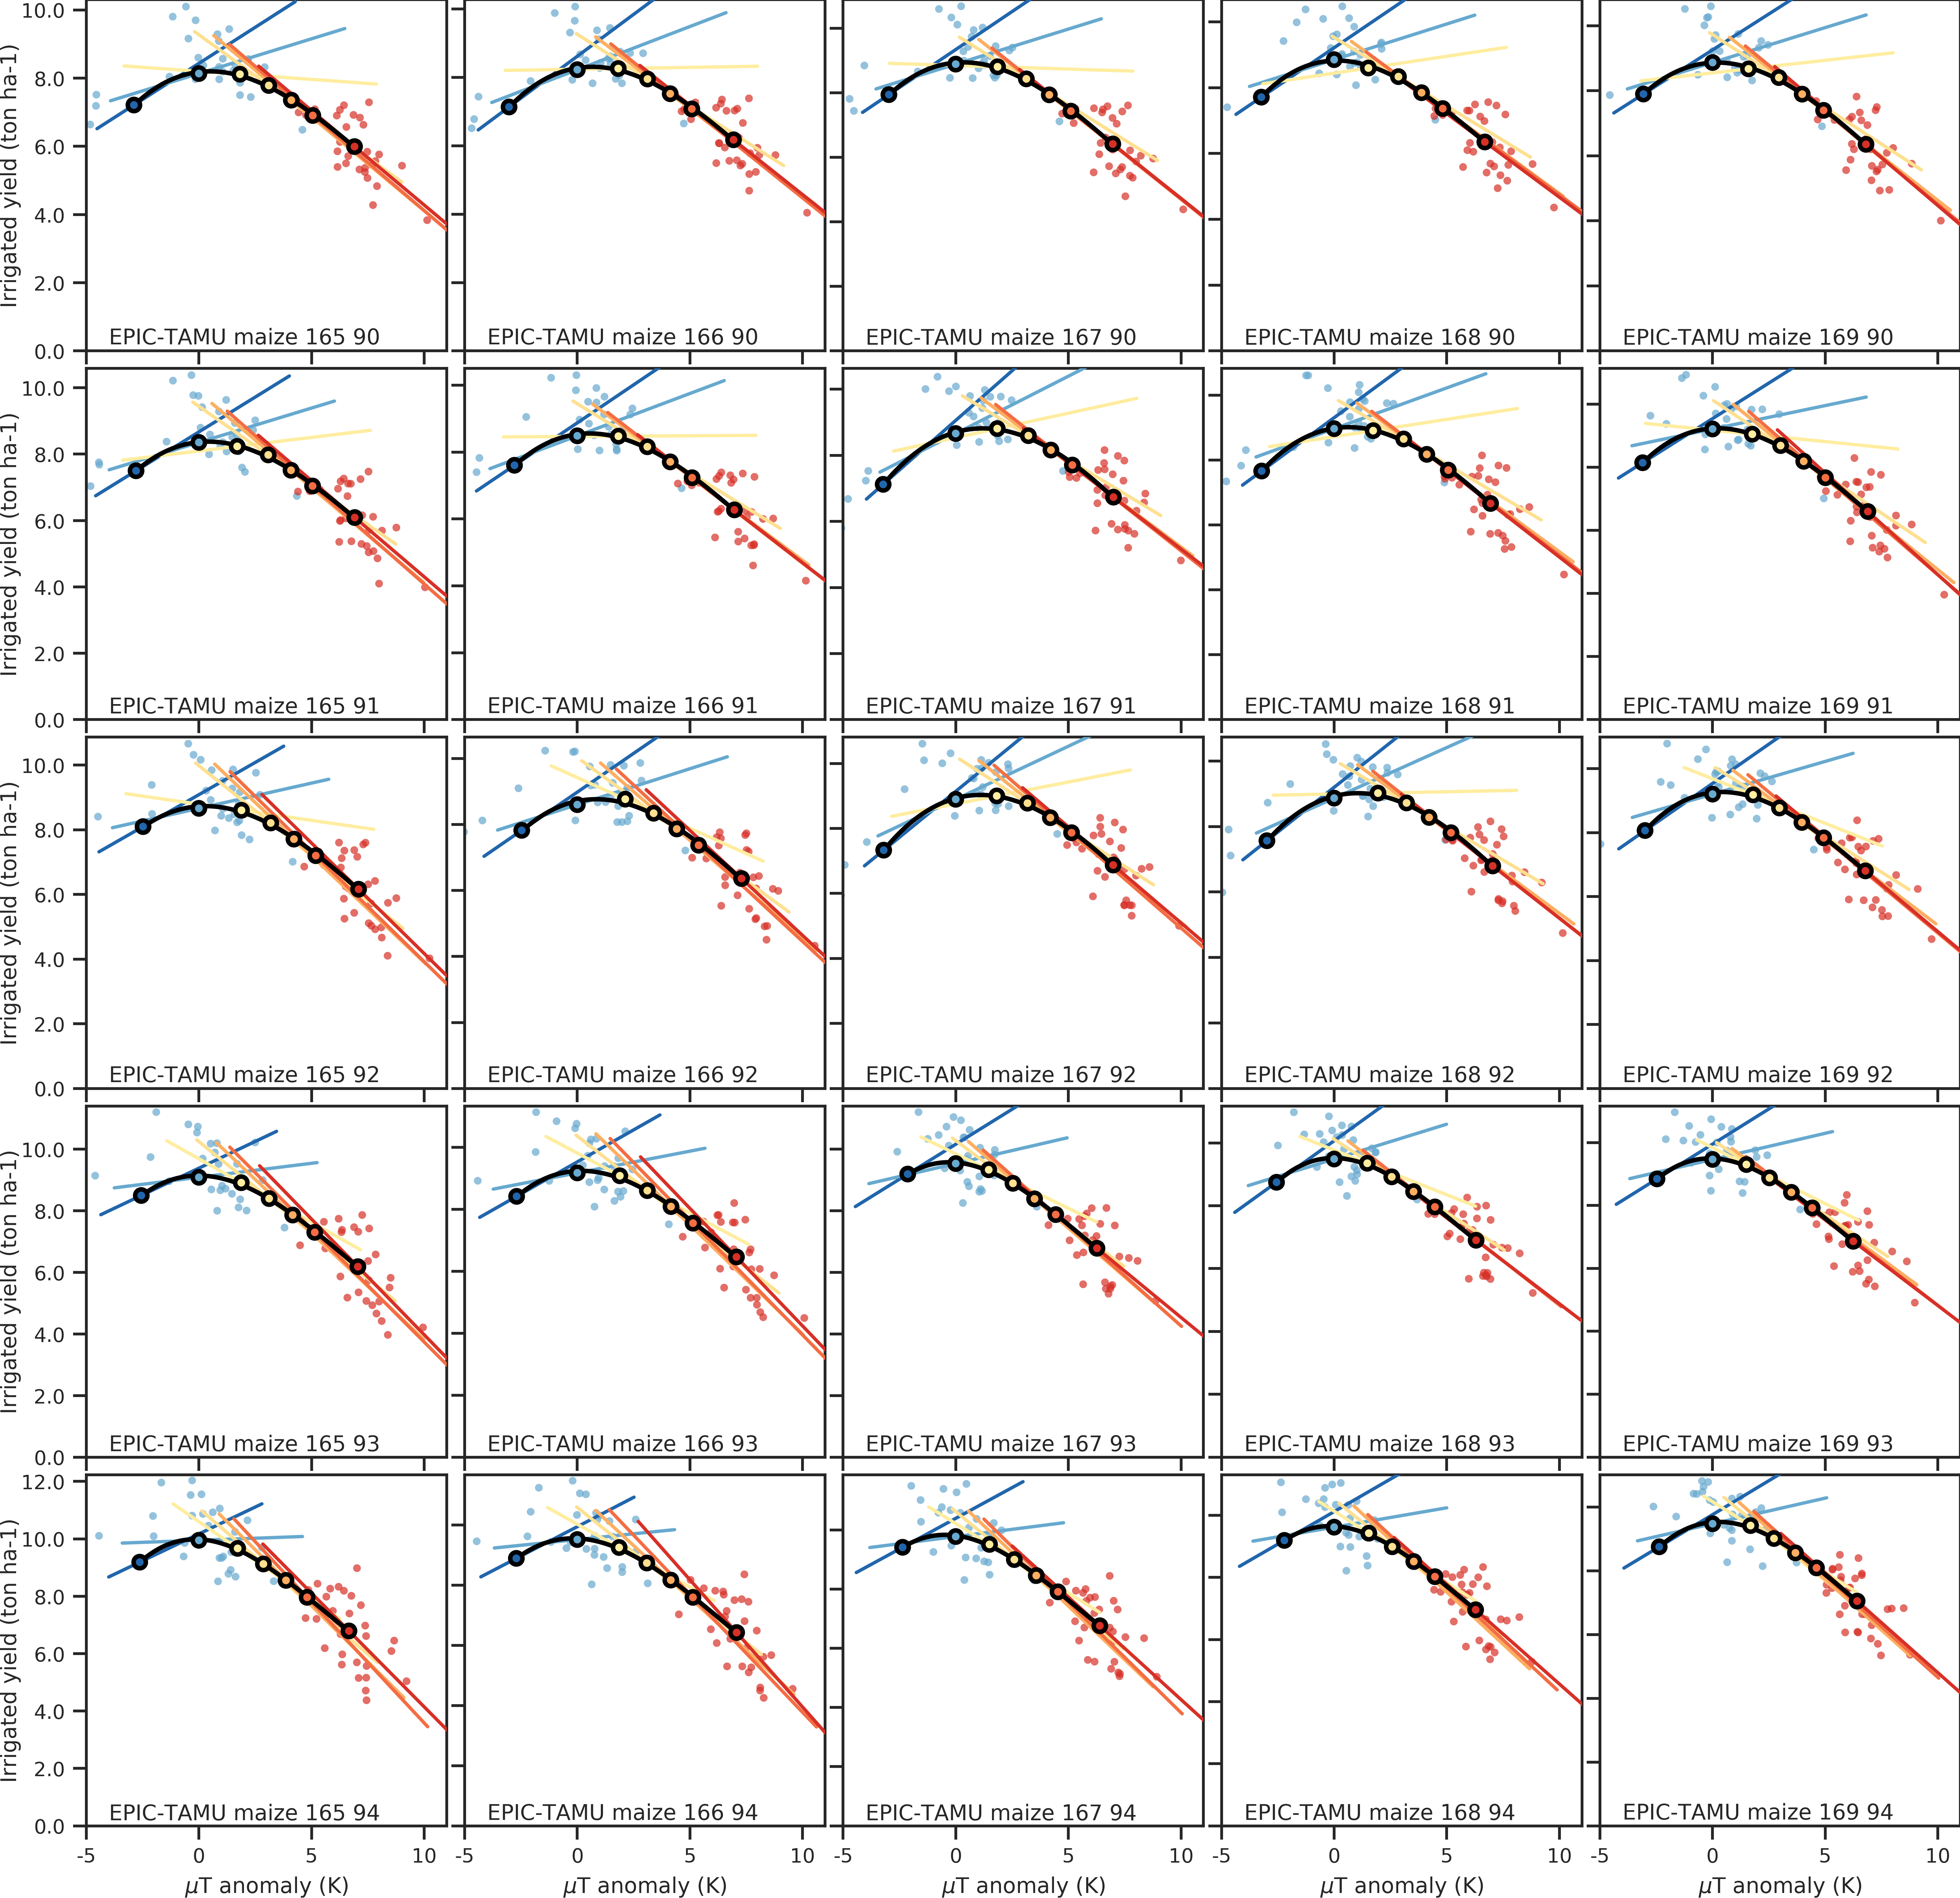
\includegraphics[width=\textwidth]{tempyearvclim_maize_EPIC-TAMU.png}
\caption{Same convention as main text Figure 1 except for multiple gricells in iowa for maize for the EPIC-TAMU model.}
\label{fig:epicmaize}
\end{figure}

\begin{figure}[h!]
%S5
\centering
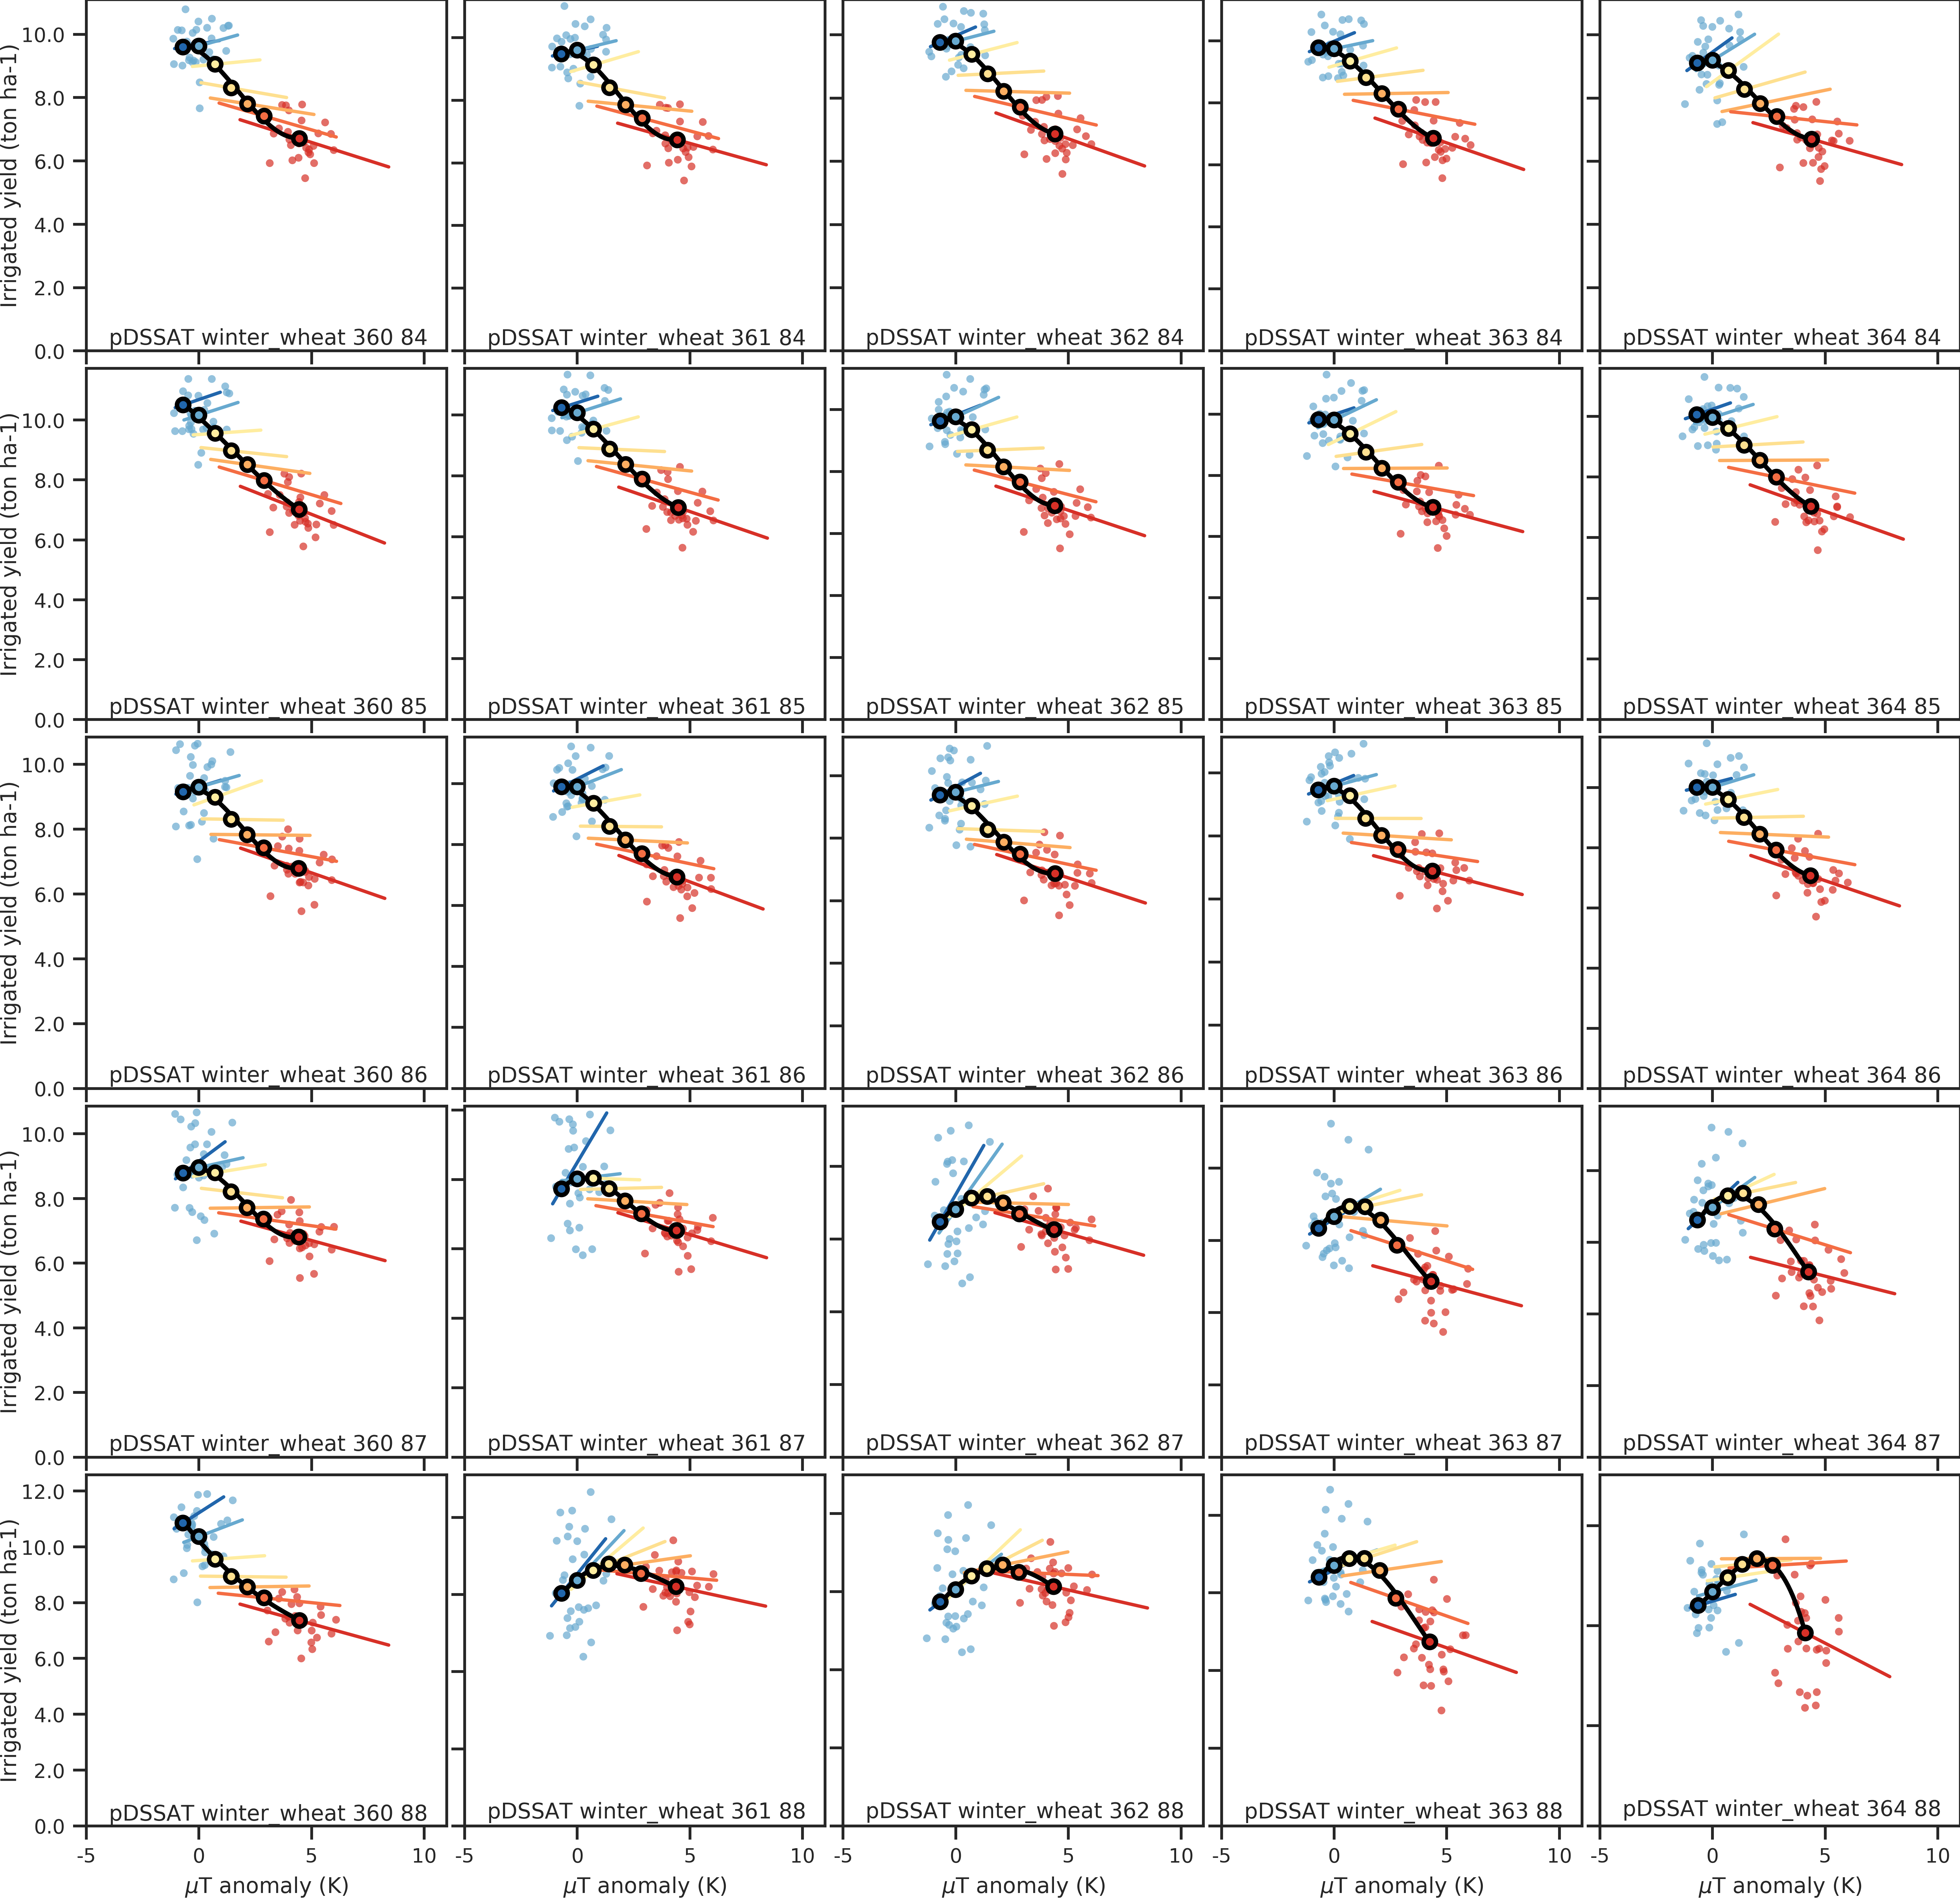
\includegraphics[width=\textwidth]{tempyearvclim_winter_wheat_pDSSAT.png}
\caption{Same convention as above except for winter wheat in France for the pDSSAT model.}
\label{fig:pdssatwwh}
\end{figure}

\begin{figure}[h!]
%S6
\centering
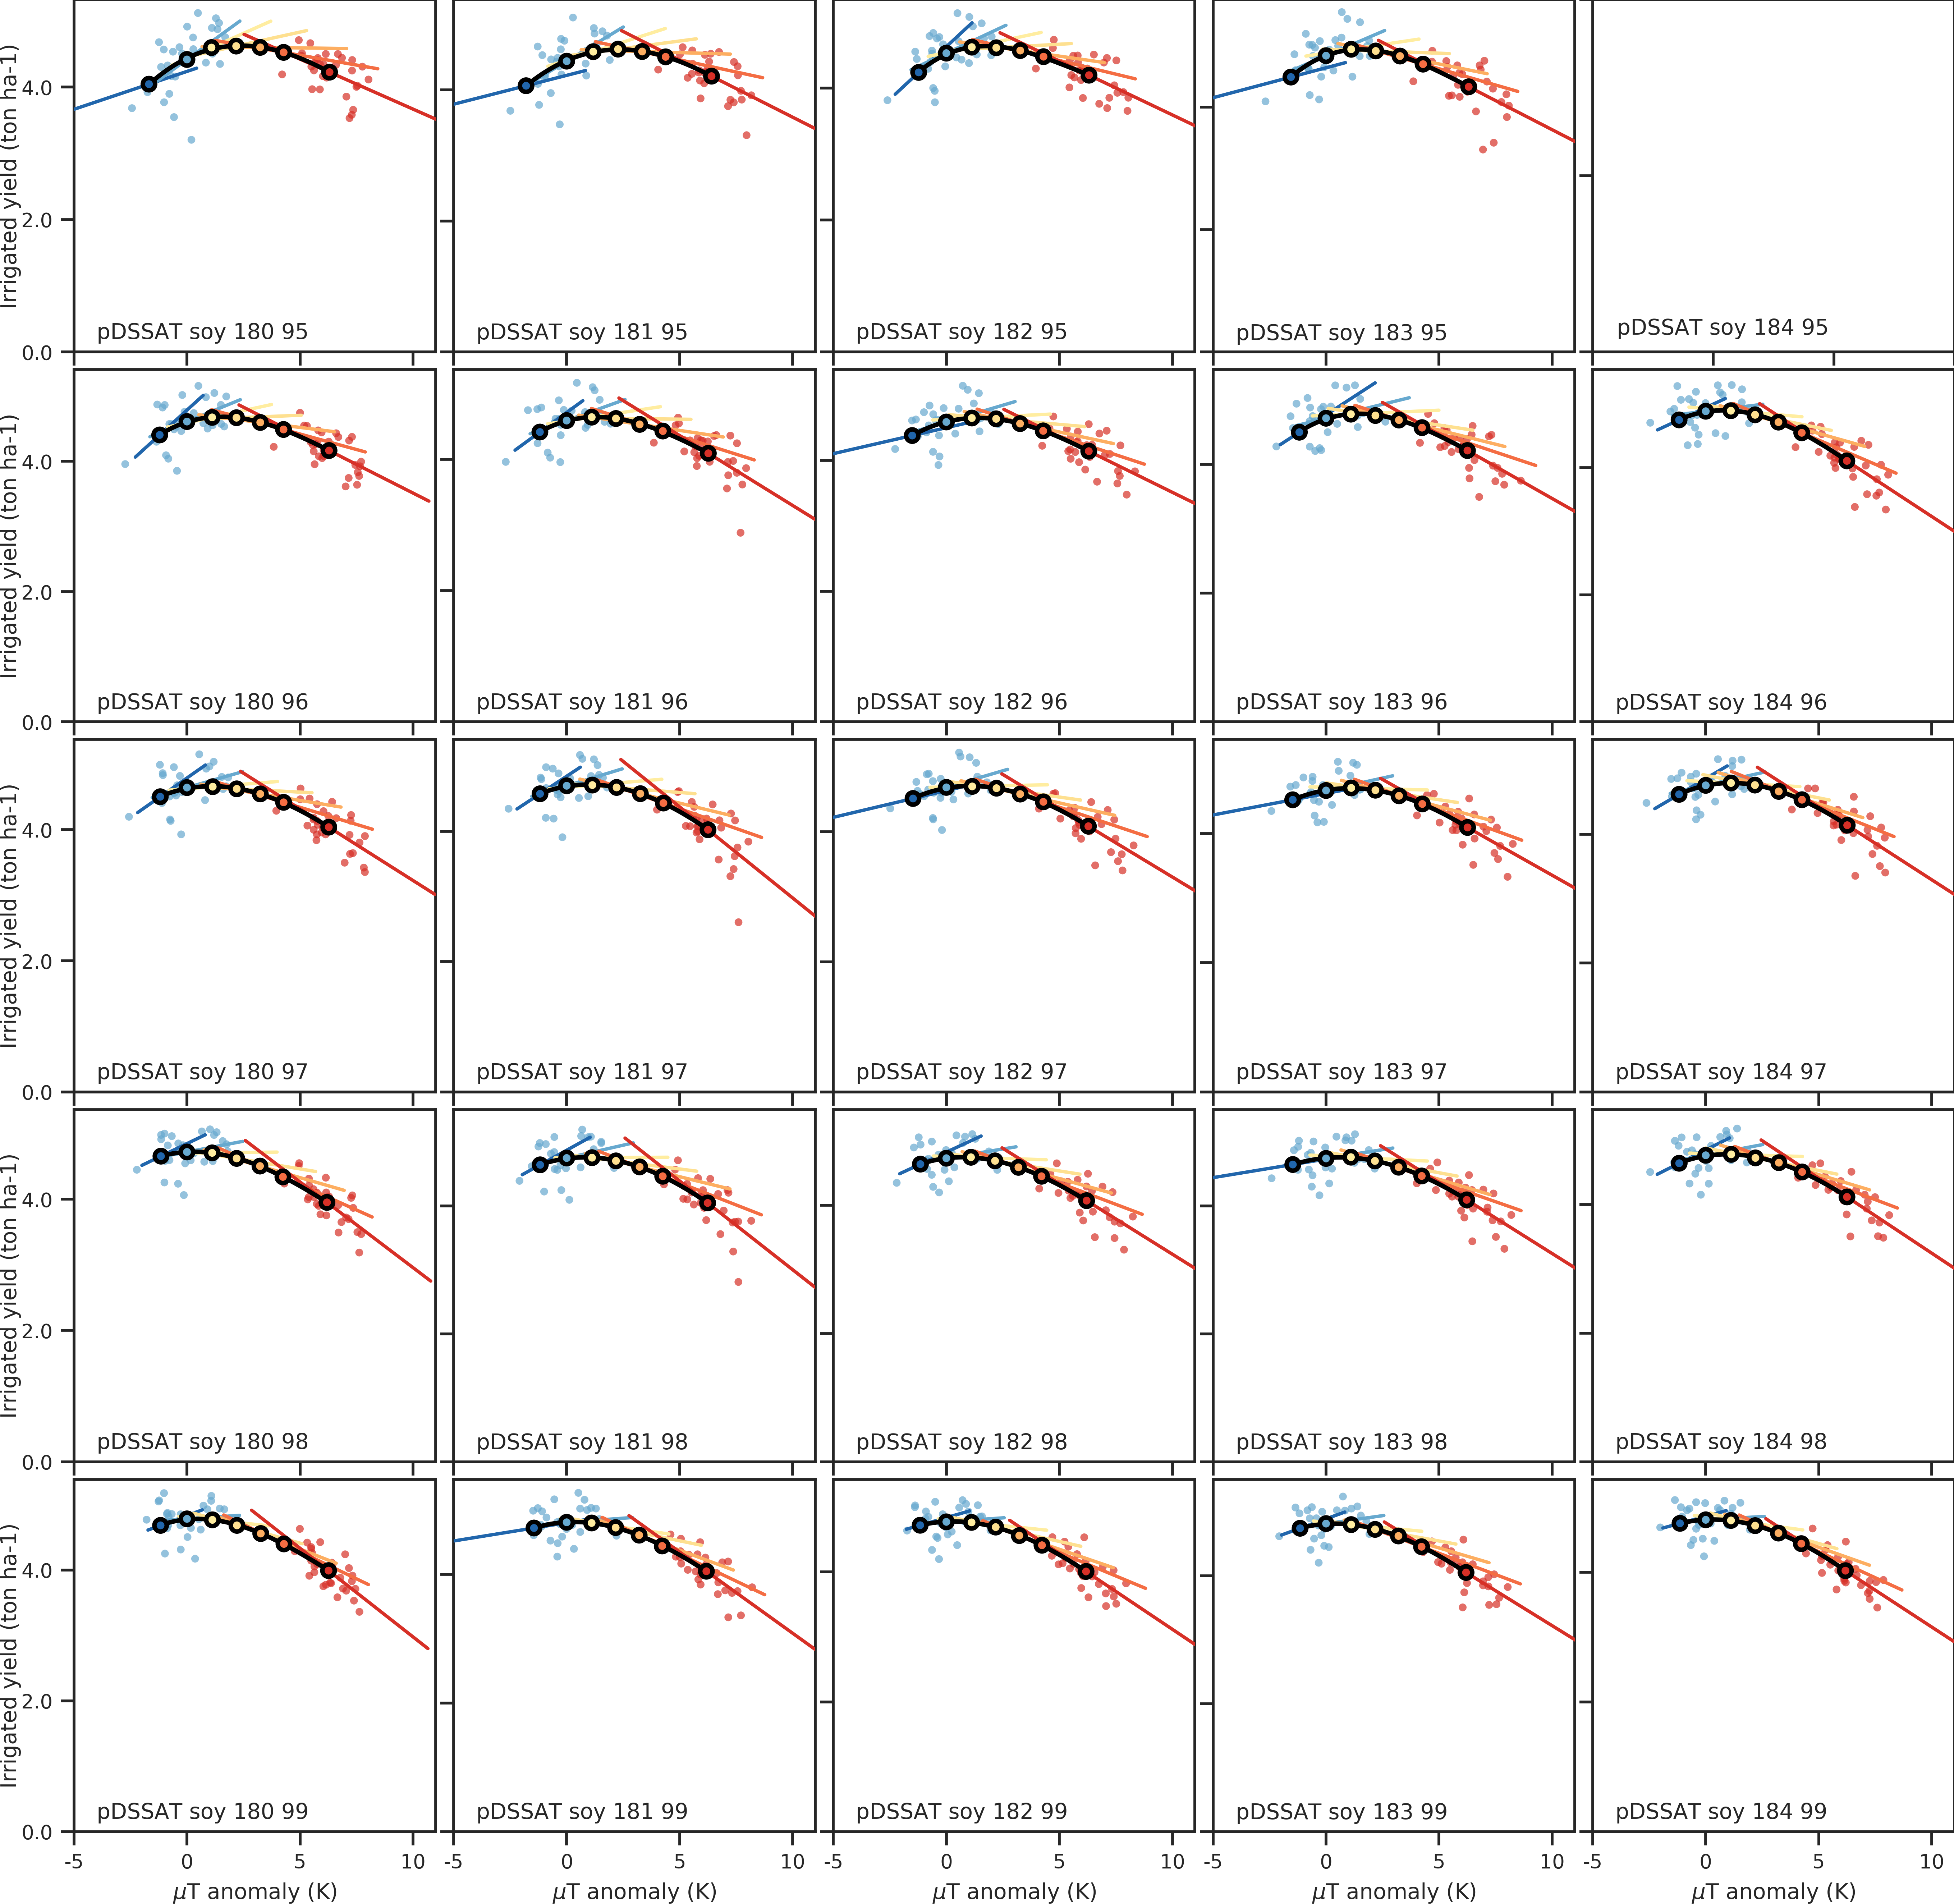
\includegraphics[width=\textwidth]{tempyearvclim_soy_pDSSAT.png}
\caption{Same convention as above except for soy in Illinois for the pDSSAT model.}
\label{fig:pdssatsoy}
\end{figure}

\begin{figure}[h!]
%S7
\centering
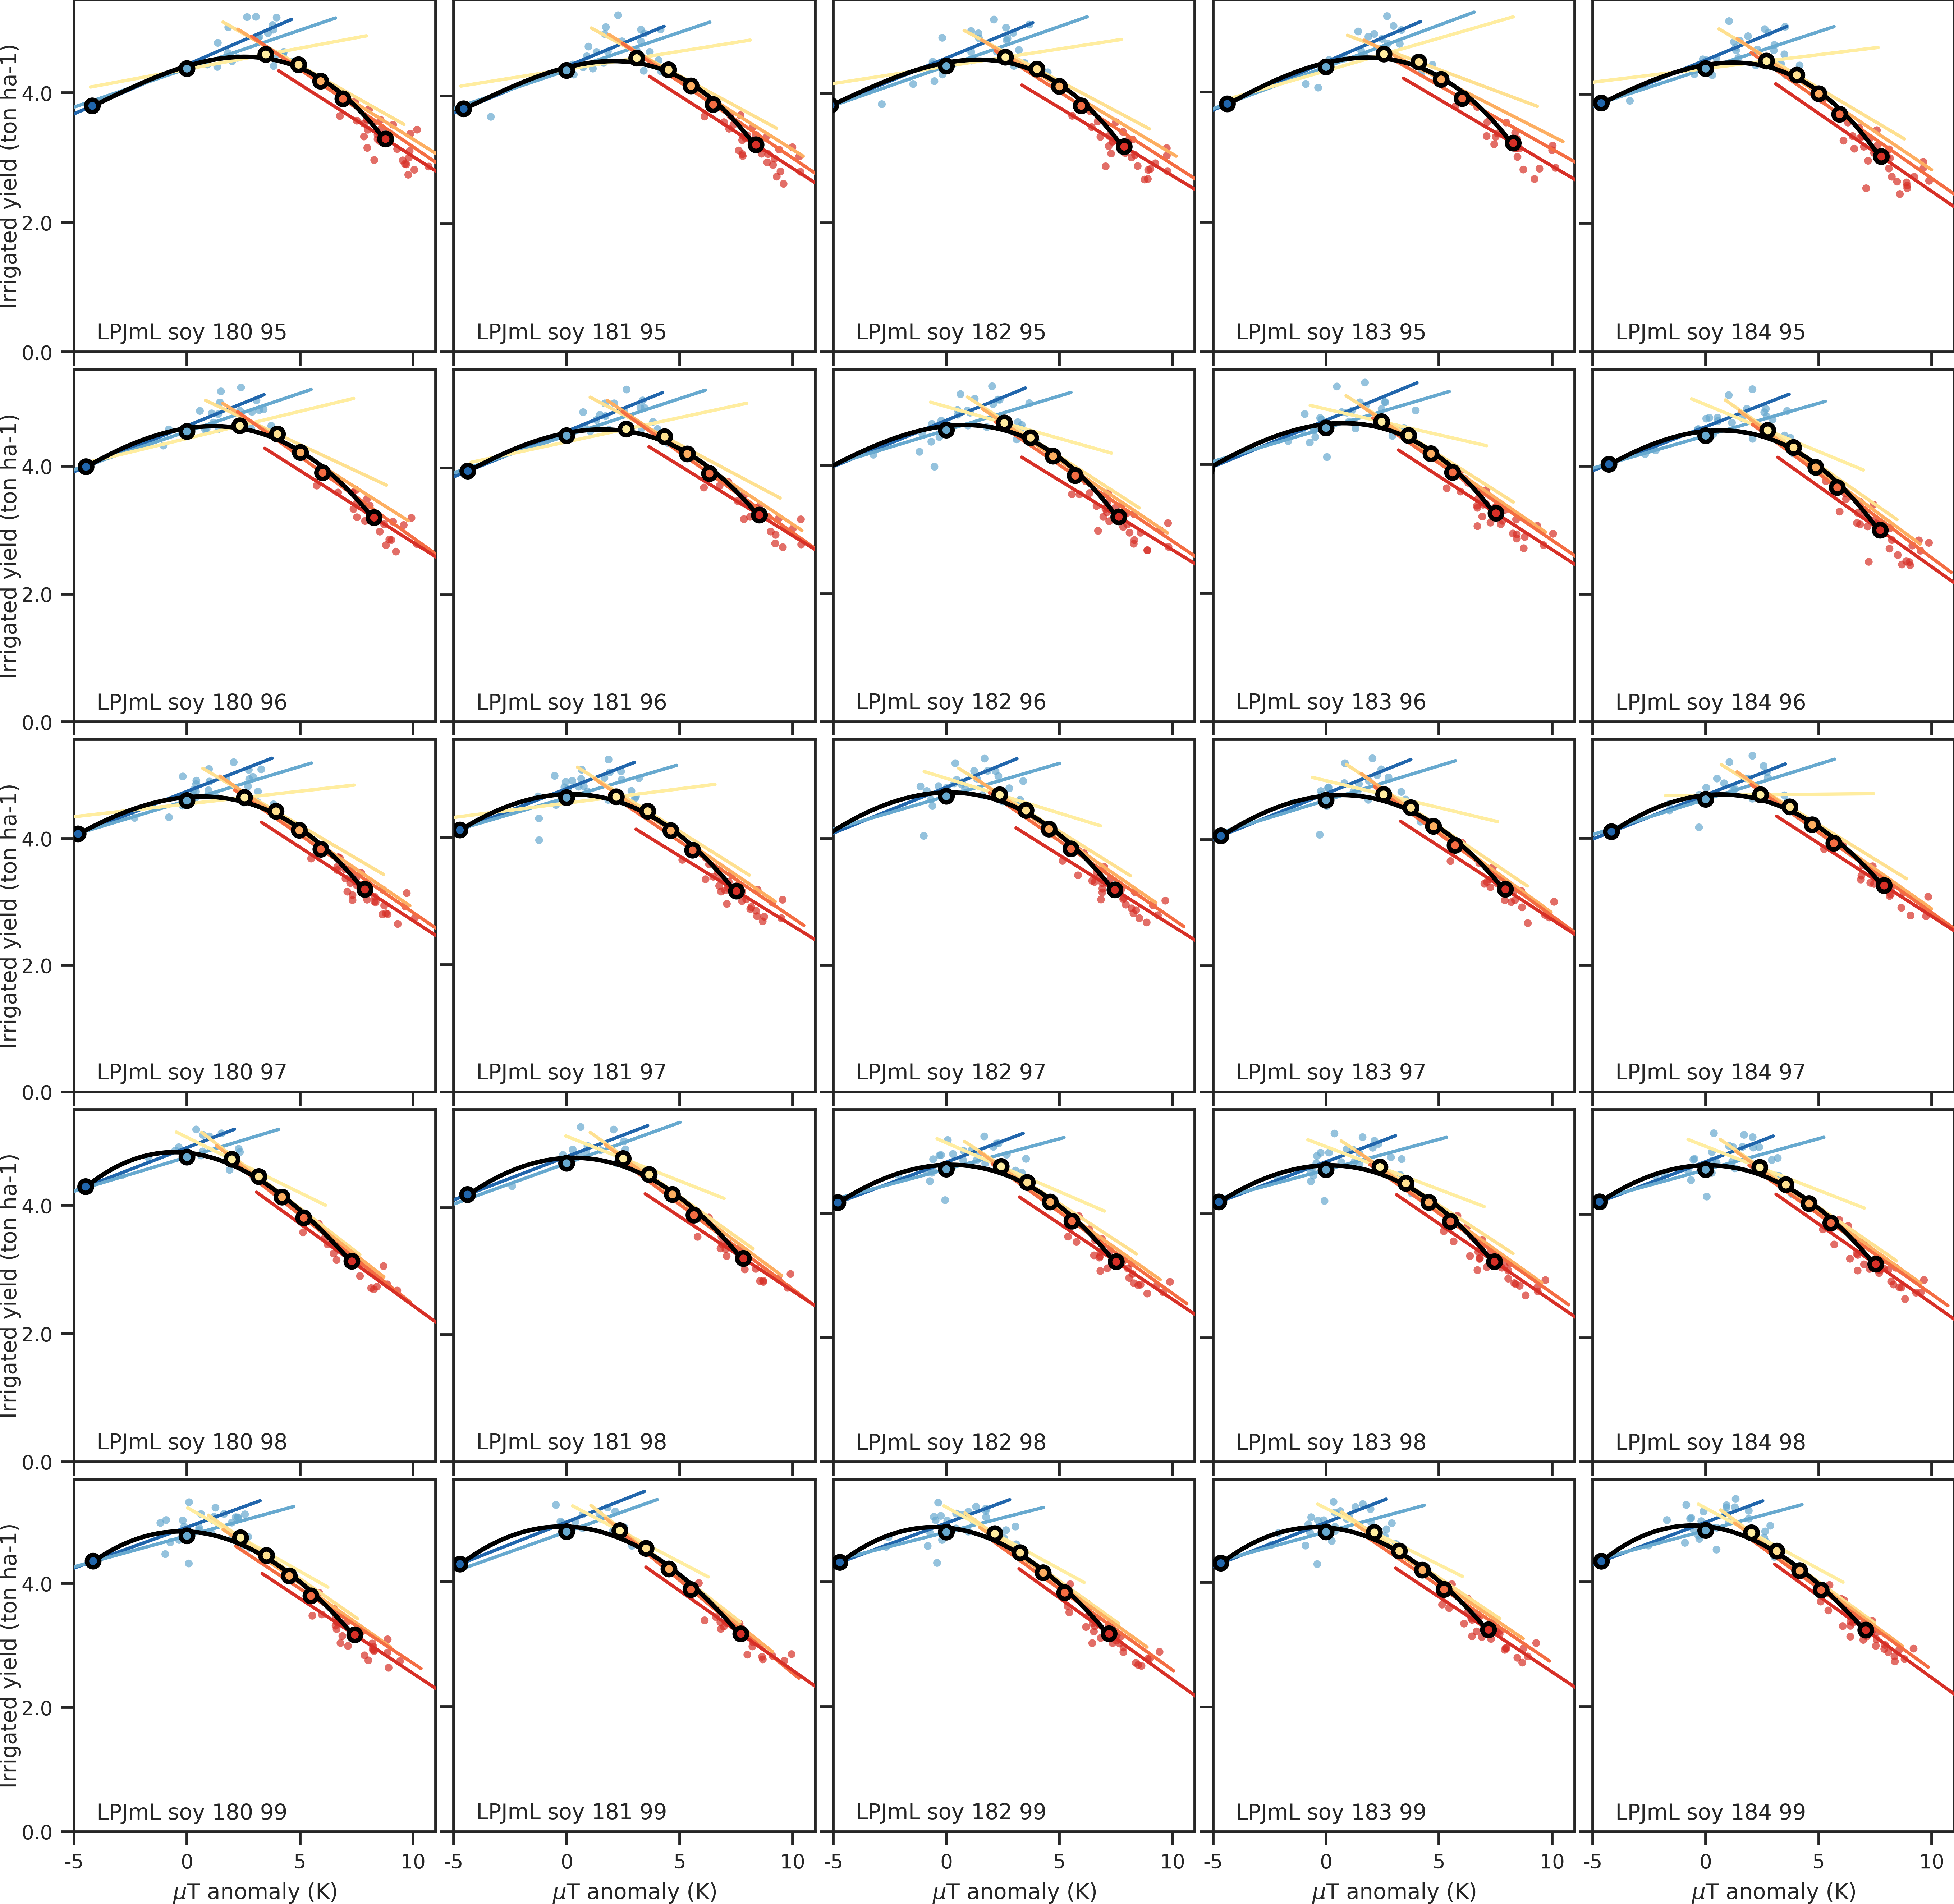
\includegraphics[width=\textwidth]{tempyearvclim_soy_LPJmL.png}
\caption{Same convention as above except for soy in Illinois for the LPJmL model.}
\label{fig:lpjmlsoy}
\end{figure}

\begin{figure}[h!]
%S8
\centering
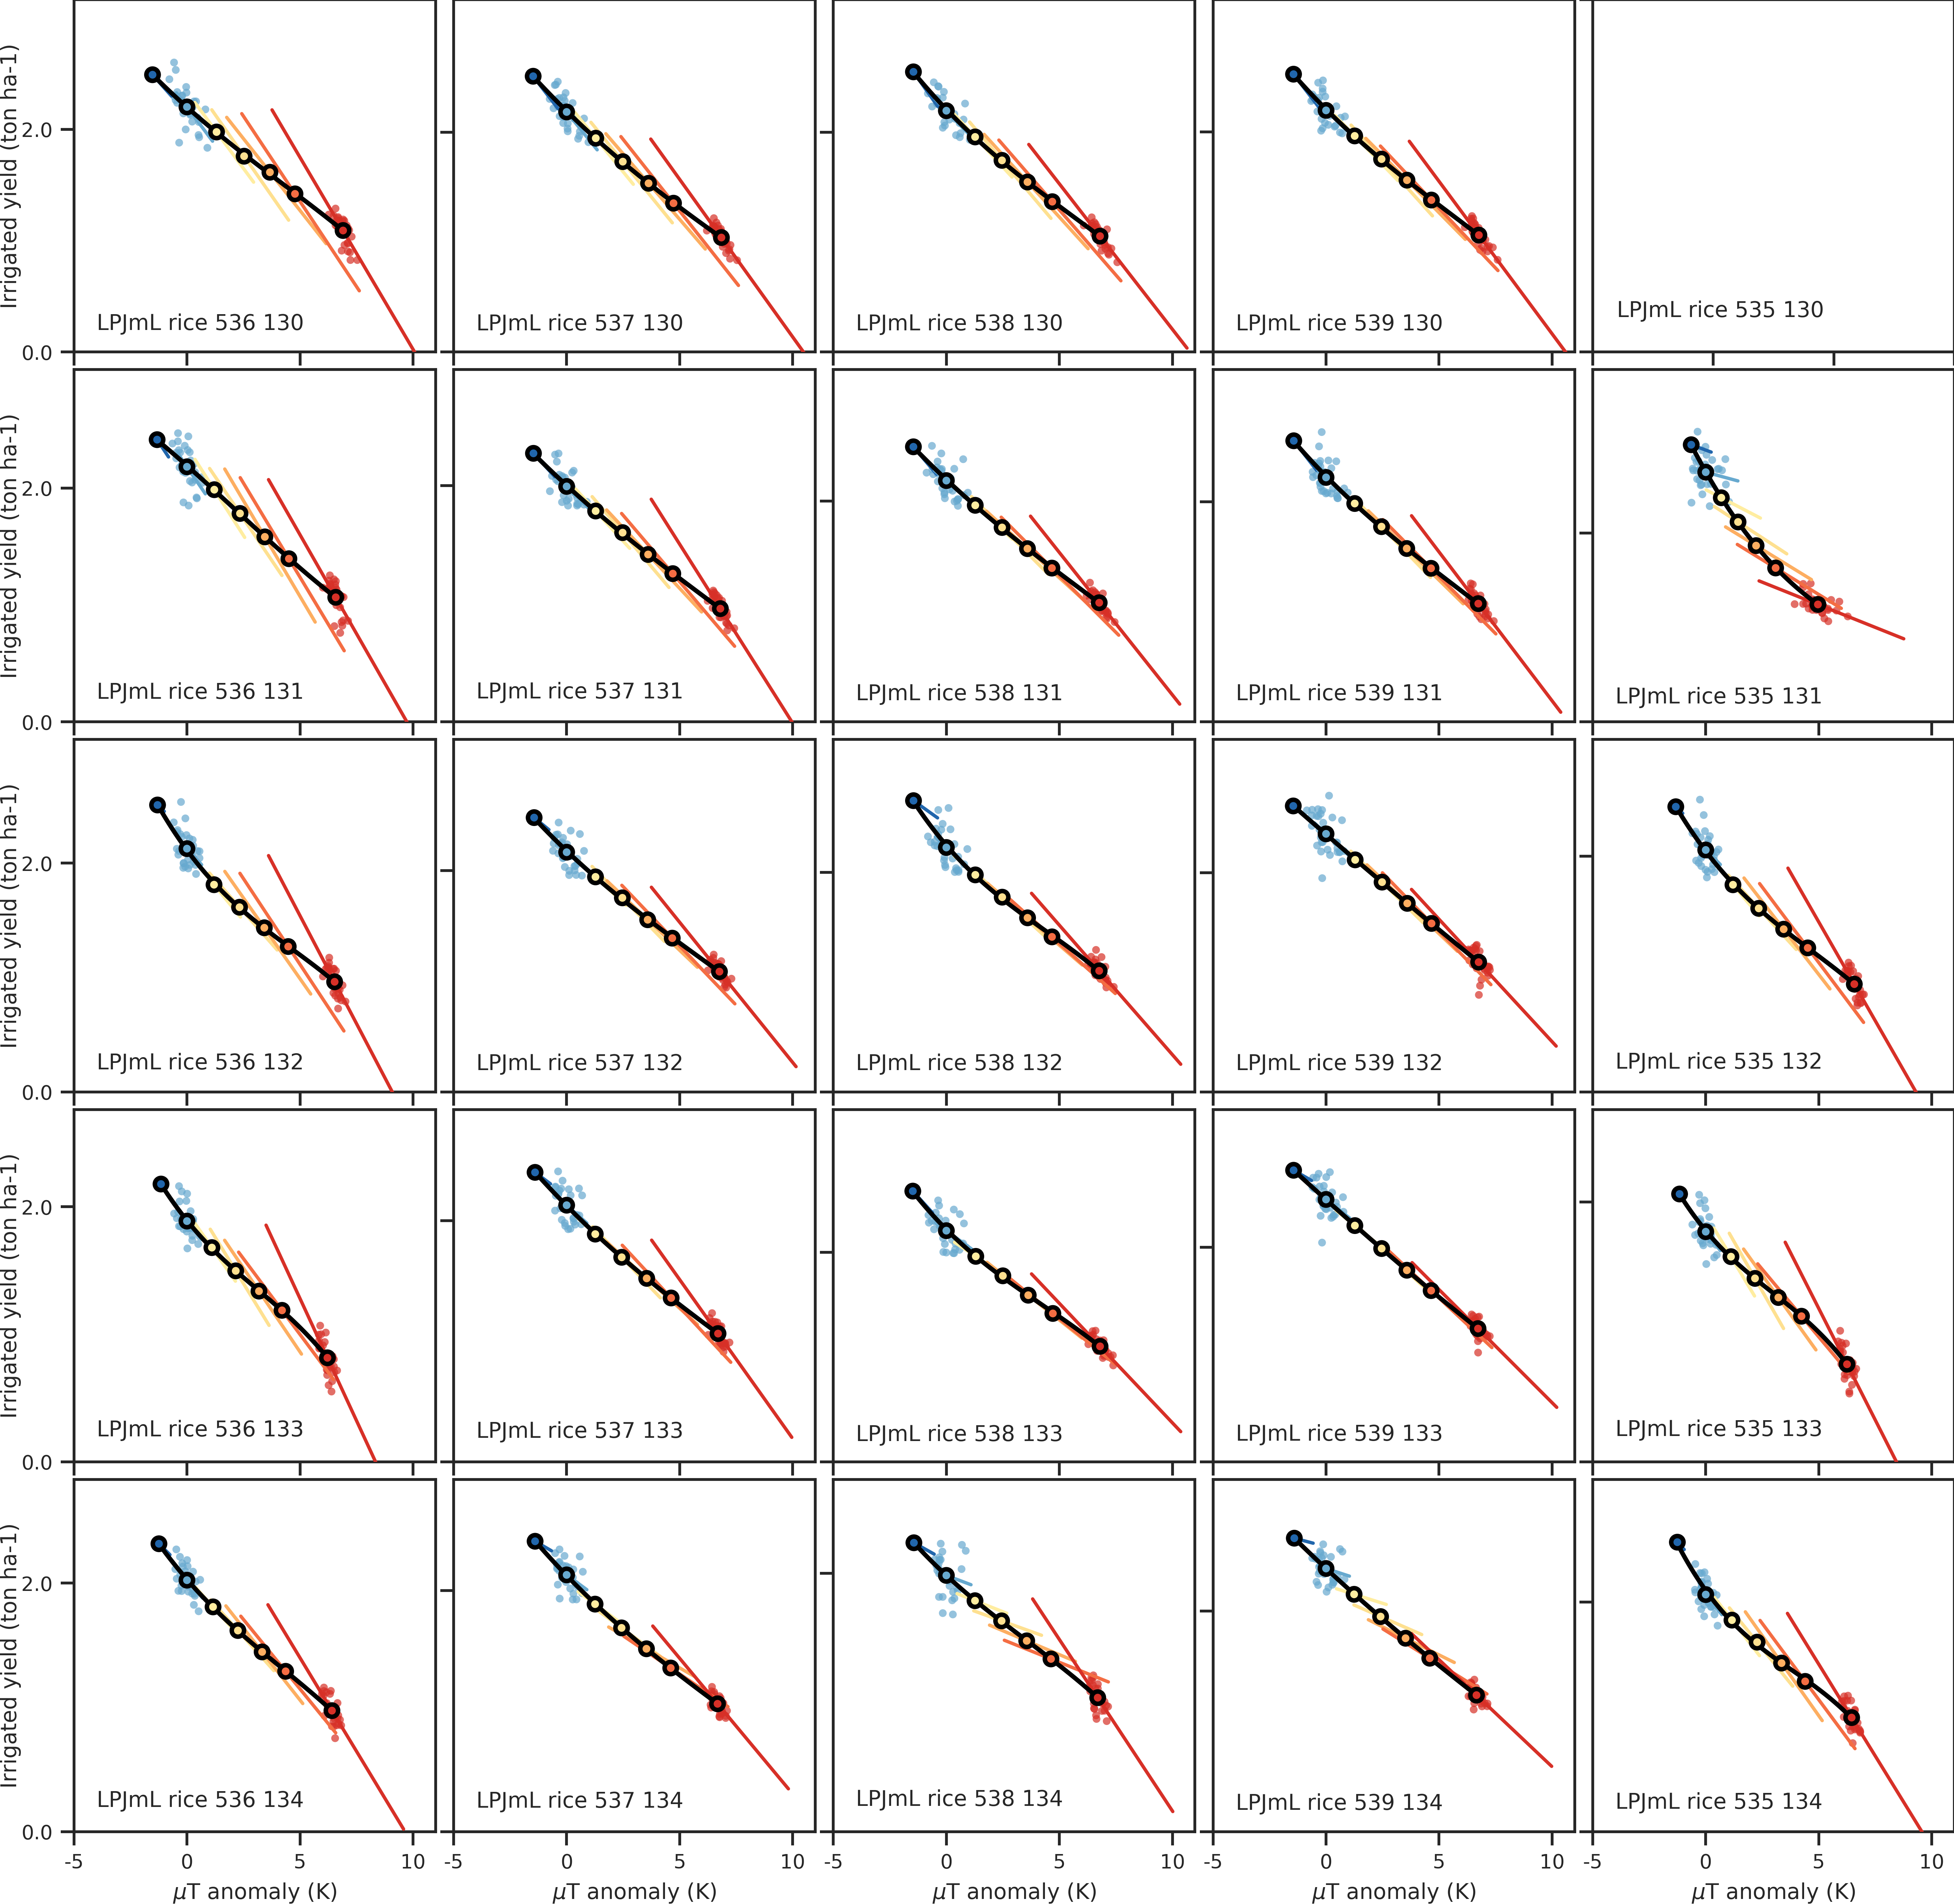
\includegraphics[width=\textwidth]{tempyearvclim_rice_LPJmL.png}
\caption{Same convention as above except for rice in India/Bangladesh for the LPJmL model.}
\label{fig:lpjmlrice}
\end{figure}

%%%%%%%%%%%%%%%%%%%%%%%%%%%%%%%%%%%%%%%%%%%%%%%%%%%%%%%%%%%%%%%%%%%%%%%%%%%%%%%%%%%%%%%
%%%%%%%%%%%%%%%%%%%%%%%%%%%%%%%%%%%%%%%%%%%%%%%%%%%%%%%%%%%%%%%%%%%%%%%%%%%%%%%%%%%%%%%
%%%%%%%%%%%%%%%%%%%%%%%%%%%%%%%%%%%%%%%%%%%%%%%%%%%%%%%%%%%%%%%%%%%%%%%%%%%%%%%%%%%%%%%
\clearpage
\subsection{Yield Response}
\begin{figure}[h!]
%S9
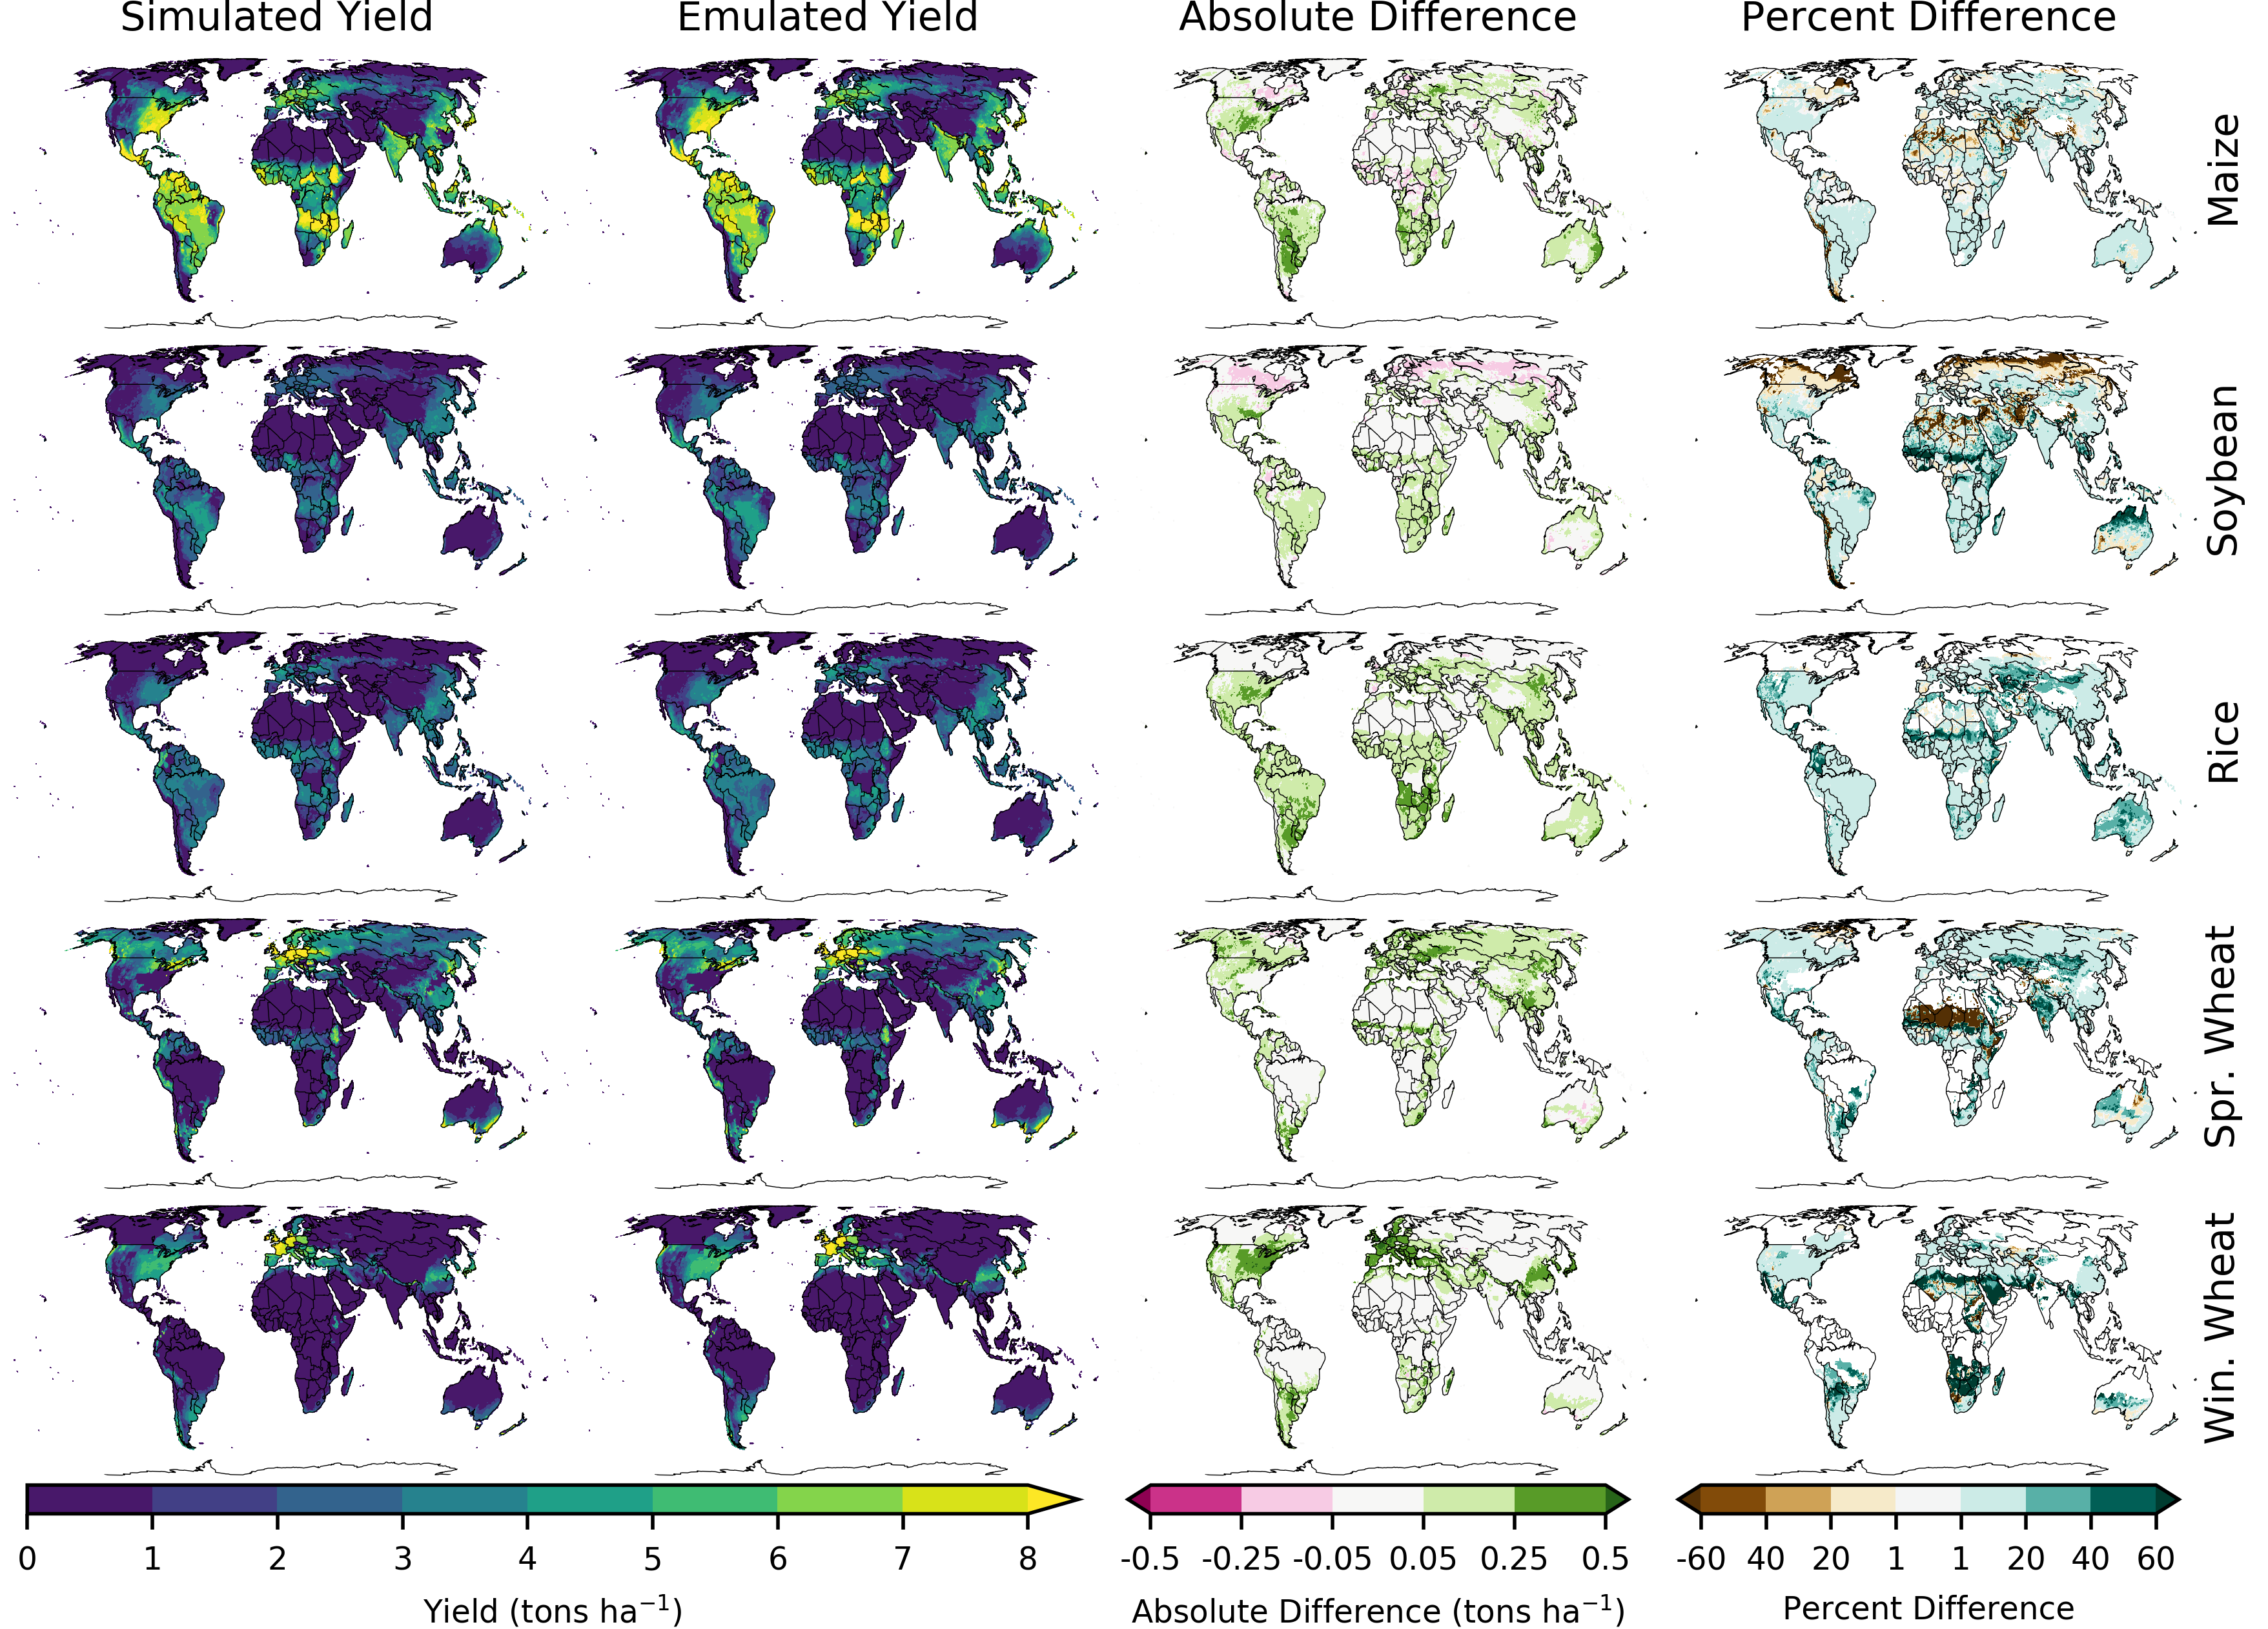
\includegraphics[width=\textwidth]{lpjml_grid.png}
\caption{Same convention as Figure 4 in the main text except now for all crops.}
\label{fig:lpjmlrice}
\end{figure}

%%%%%%%%%%%%%%%%%%%%%%%%%%%%%%%%%%%%%%%%%%%%%%%%%%%%%%%%%%%%%%%%%%%%%%%%%%%%%%%%%%%%%%%
%%%%%%%%%%%%%%%%%%%%%%%%%%%%%%%%%%%%%%%%%%%%%%%%%%%%%%%%%%%%%%%%%%%%%%%%%%%%%%%%%%%%%%%
%%%%%%%%%%%%%%%%%%%%%%%%%%%%%%%%%%%%%%%%%%%%%%%%%%%%%%%%%%%%%%%%%%%%%%%%%%%%%%%%%%%%%%%
\clearpage
\subsection{Normalized Error}

\begin{figure}[h!]
%S10
\centering
\begin{minipage}{.45\textwidth}
\centering
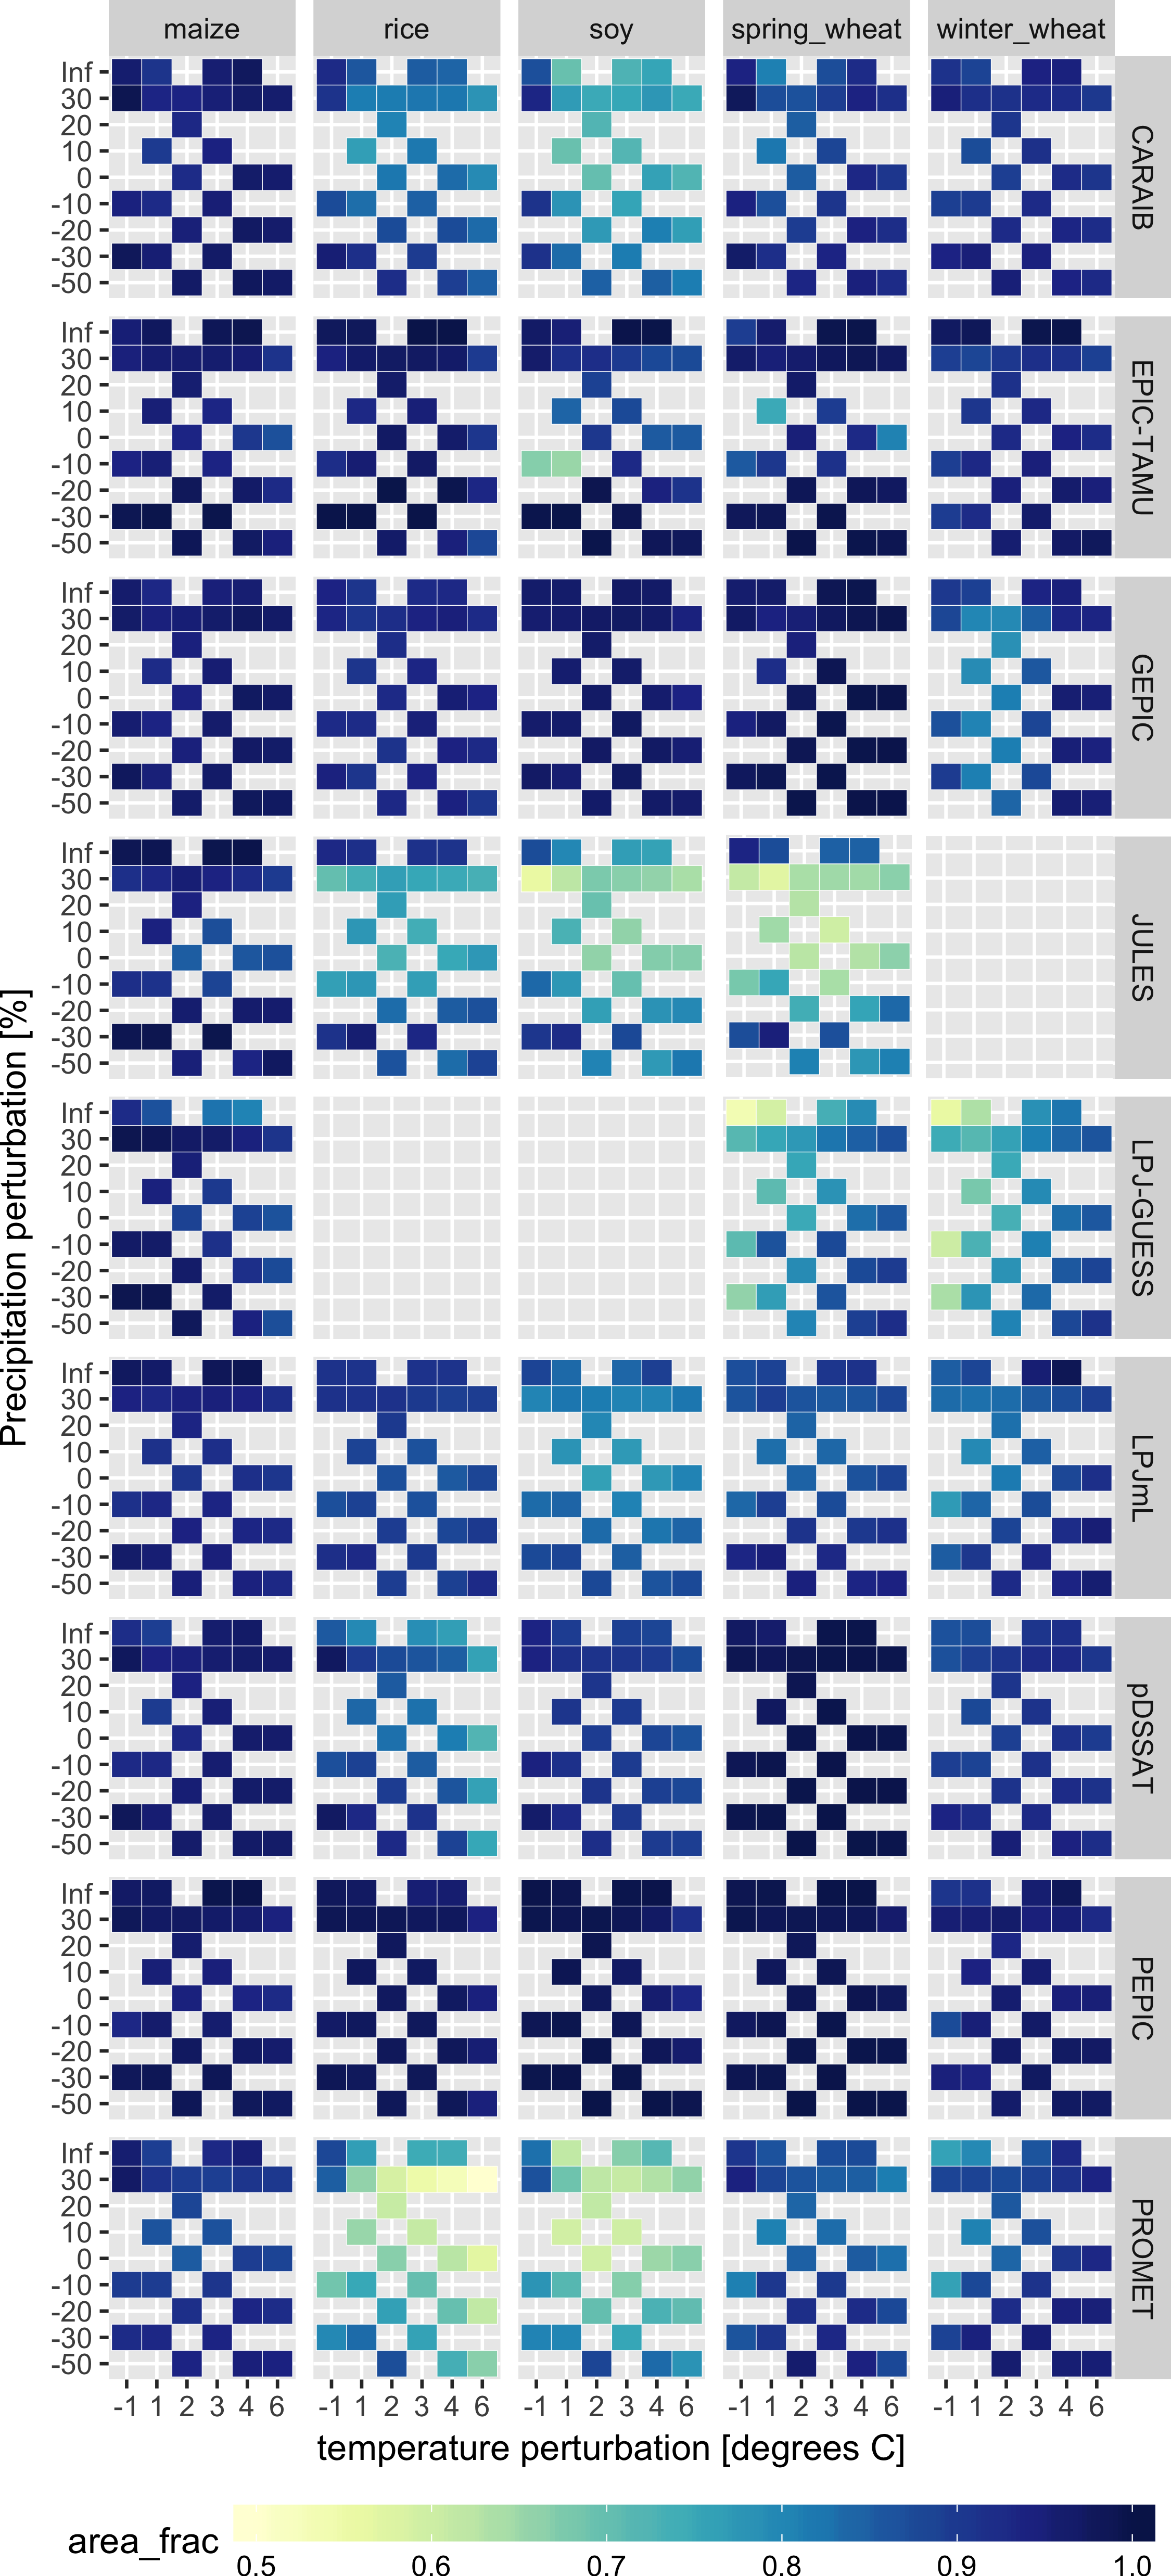
\includegraphics[width=\textwidth]{s_error_360_total.png}\\
\caption{The fraction of grid cells (across all grid cells) with normalized emulation error less than 1 for the CO$_2$=360 ppm and 200 kg~N ha$^{-1}$ yr$^{-1}$ case for the temperature and precipitation perturbations scenarios provided by all 9 models included in the emulator analysis. This is in contrast to the fraction of currently cultivated hectares shown in the C360 case in the manuscript and for the C810 case show in the supplemental material. The emulator is marginally more successful over currently cultivated areas than over all grid cells in general.}
\label{fig:error360total}
\end{minipage}
\hspace{.05\linewidth}
%S11
\begin{minipage}{.45\textwidth}
\centering
\vspace{0pt}
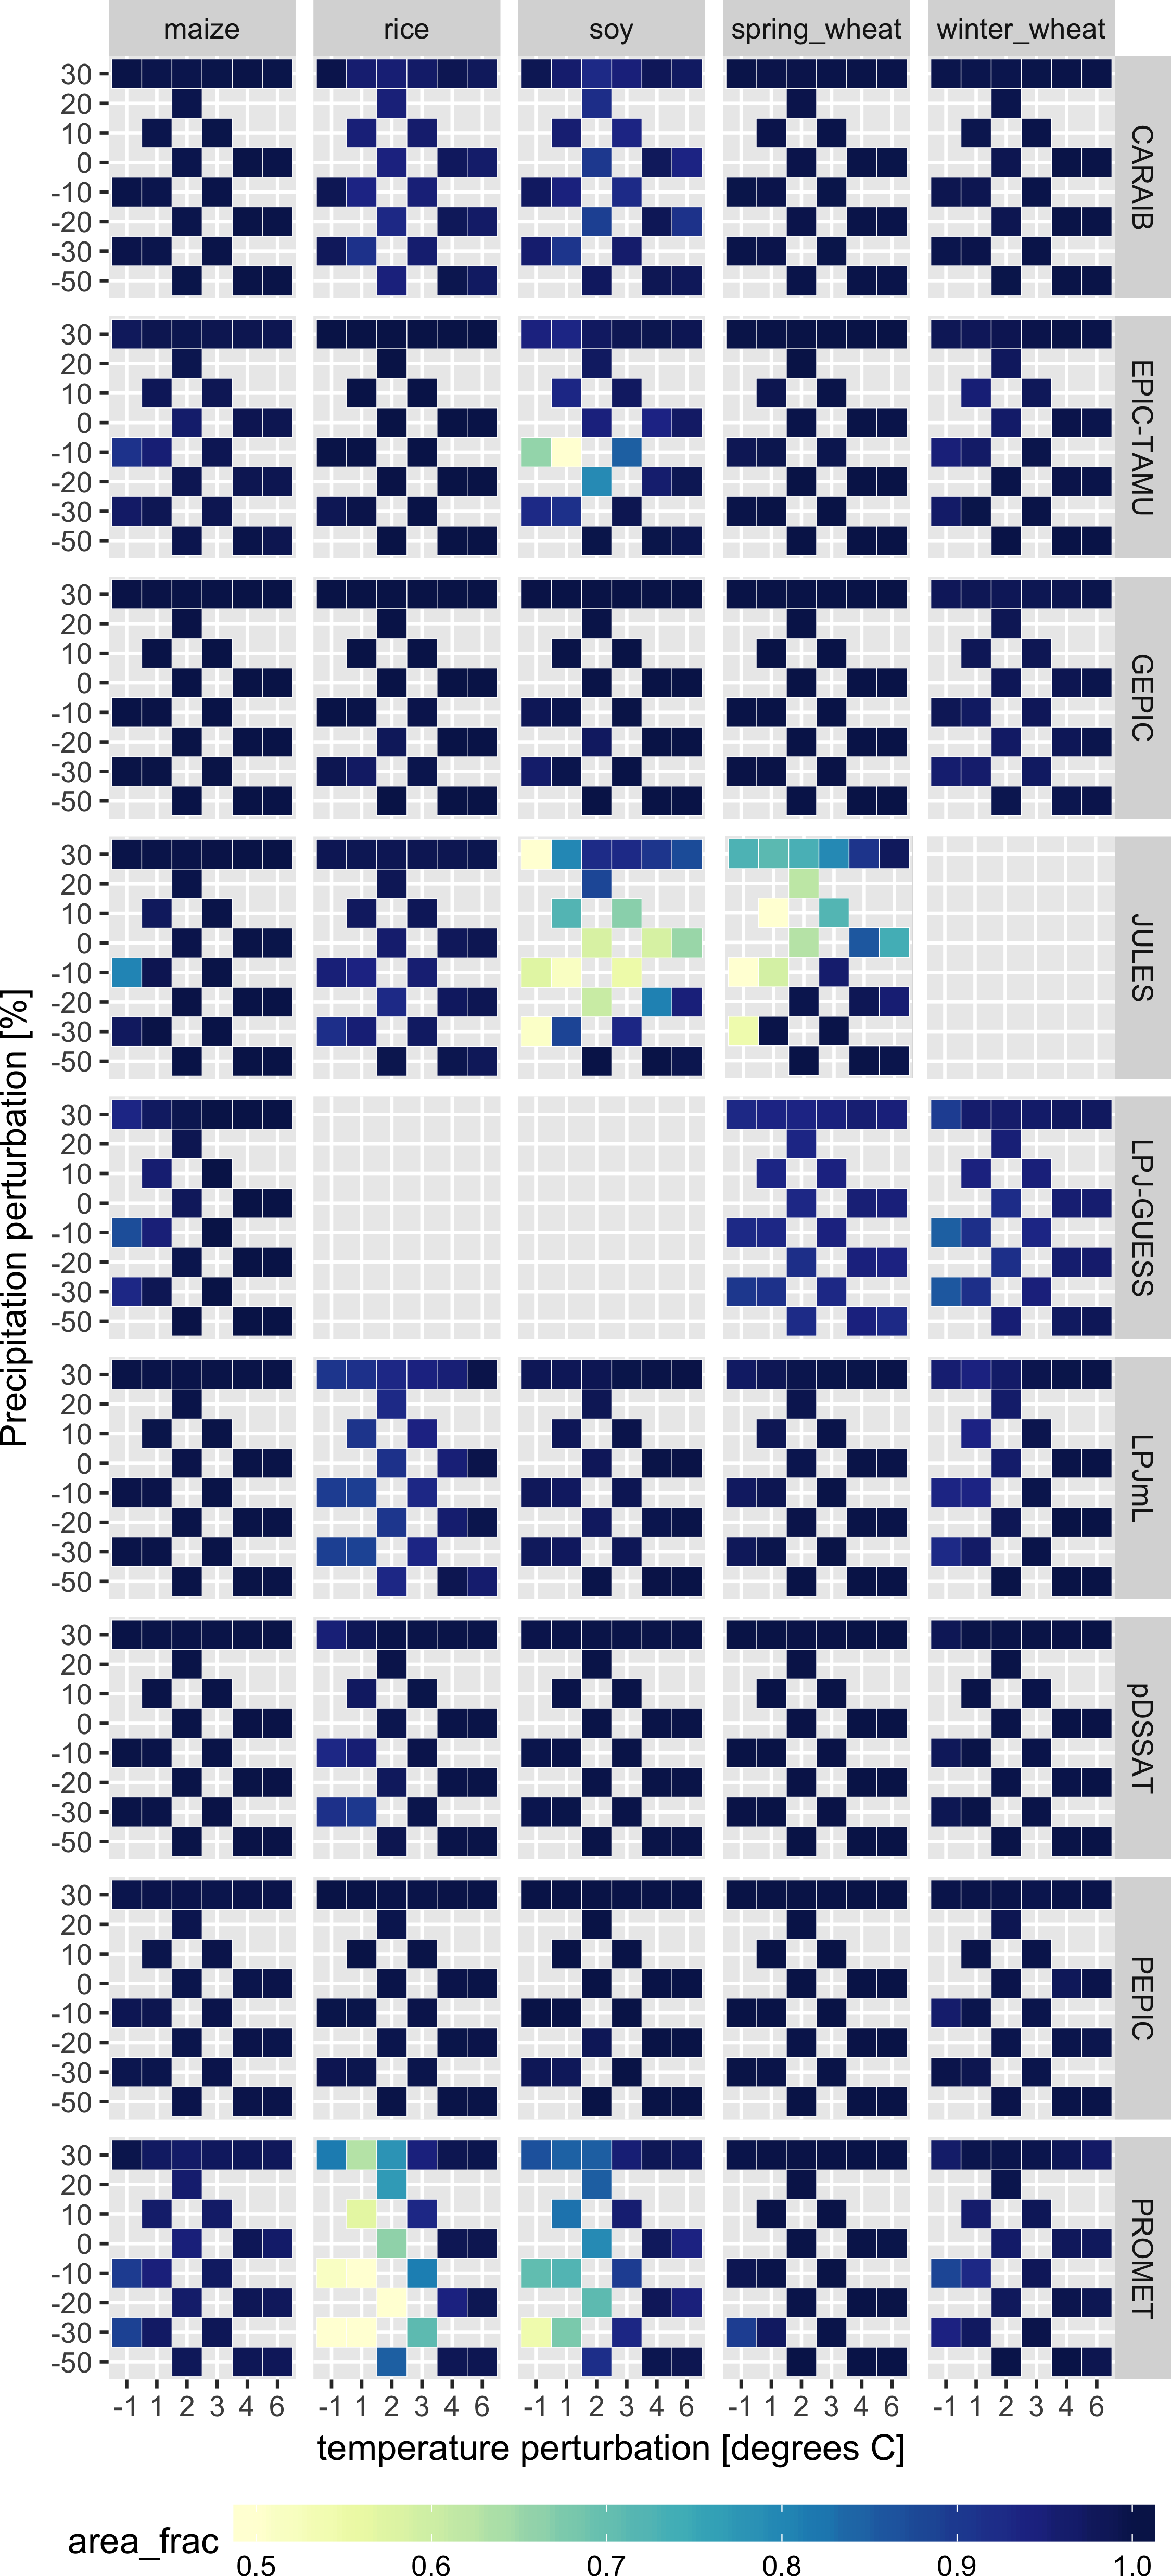
\includegraphics[width=\textwidth]{s_error_810.png}\\
\caption{The fraction of currently cultivated hectares with normalized emulation error less than 1 (blue colors contours in Figure A2) for the CO$_2$=810 ppm and 200 kg~N ha$^{-1}$ yr$^{-1}$ case for the temperature and precipitation perturbations scenarios provided by all 9 models included in the emulator analysis. See Equations A1 and A2 for normalized error calculation. The yield response is generally easy to emulate over currently cultivated areas (dark blue and light blue).}
\label{fig:error810}
\end{minipage}
\end{figure}

\begin{figure}[h!]
%S12
\centering
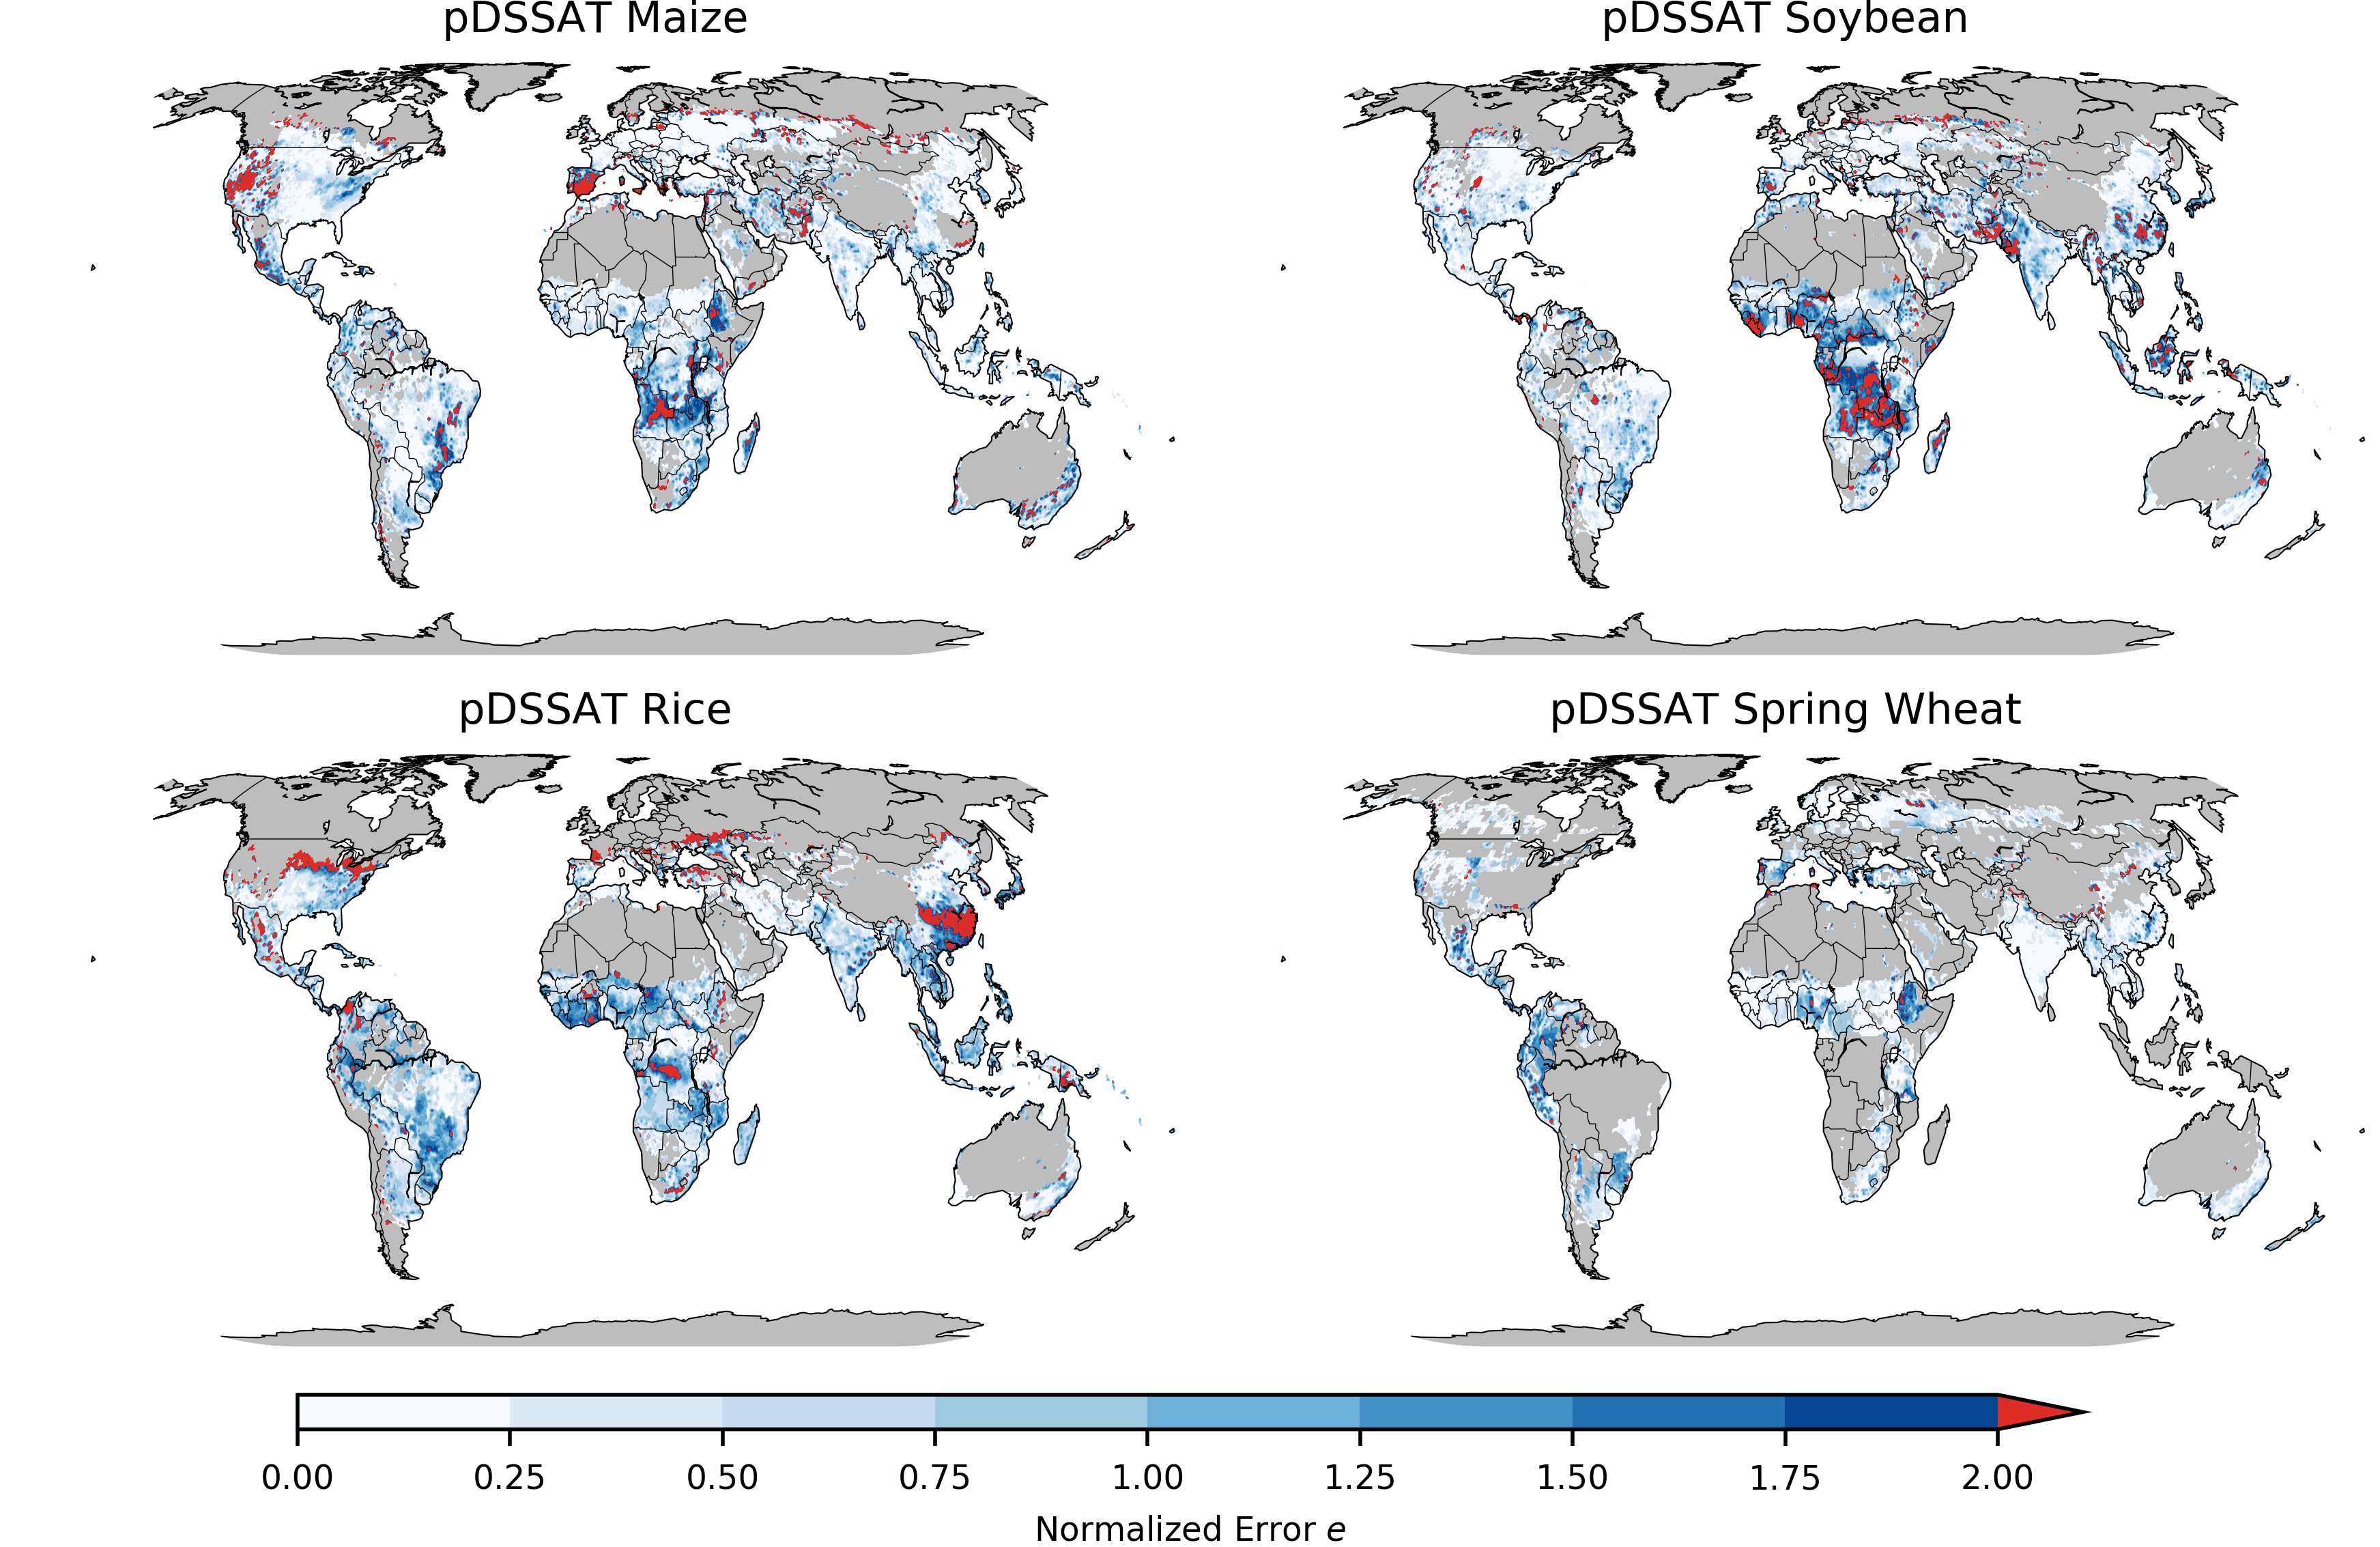
\includegraphics[width=15.5cm]{pDSSAT_spatial_error.png}
\caption{Same convention as main text Figure 8 except now for pDSSAT.}
\label{fig:pdssatnorm}
\end{figure}

\begin{figure}[h!]
%S13
\centering
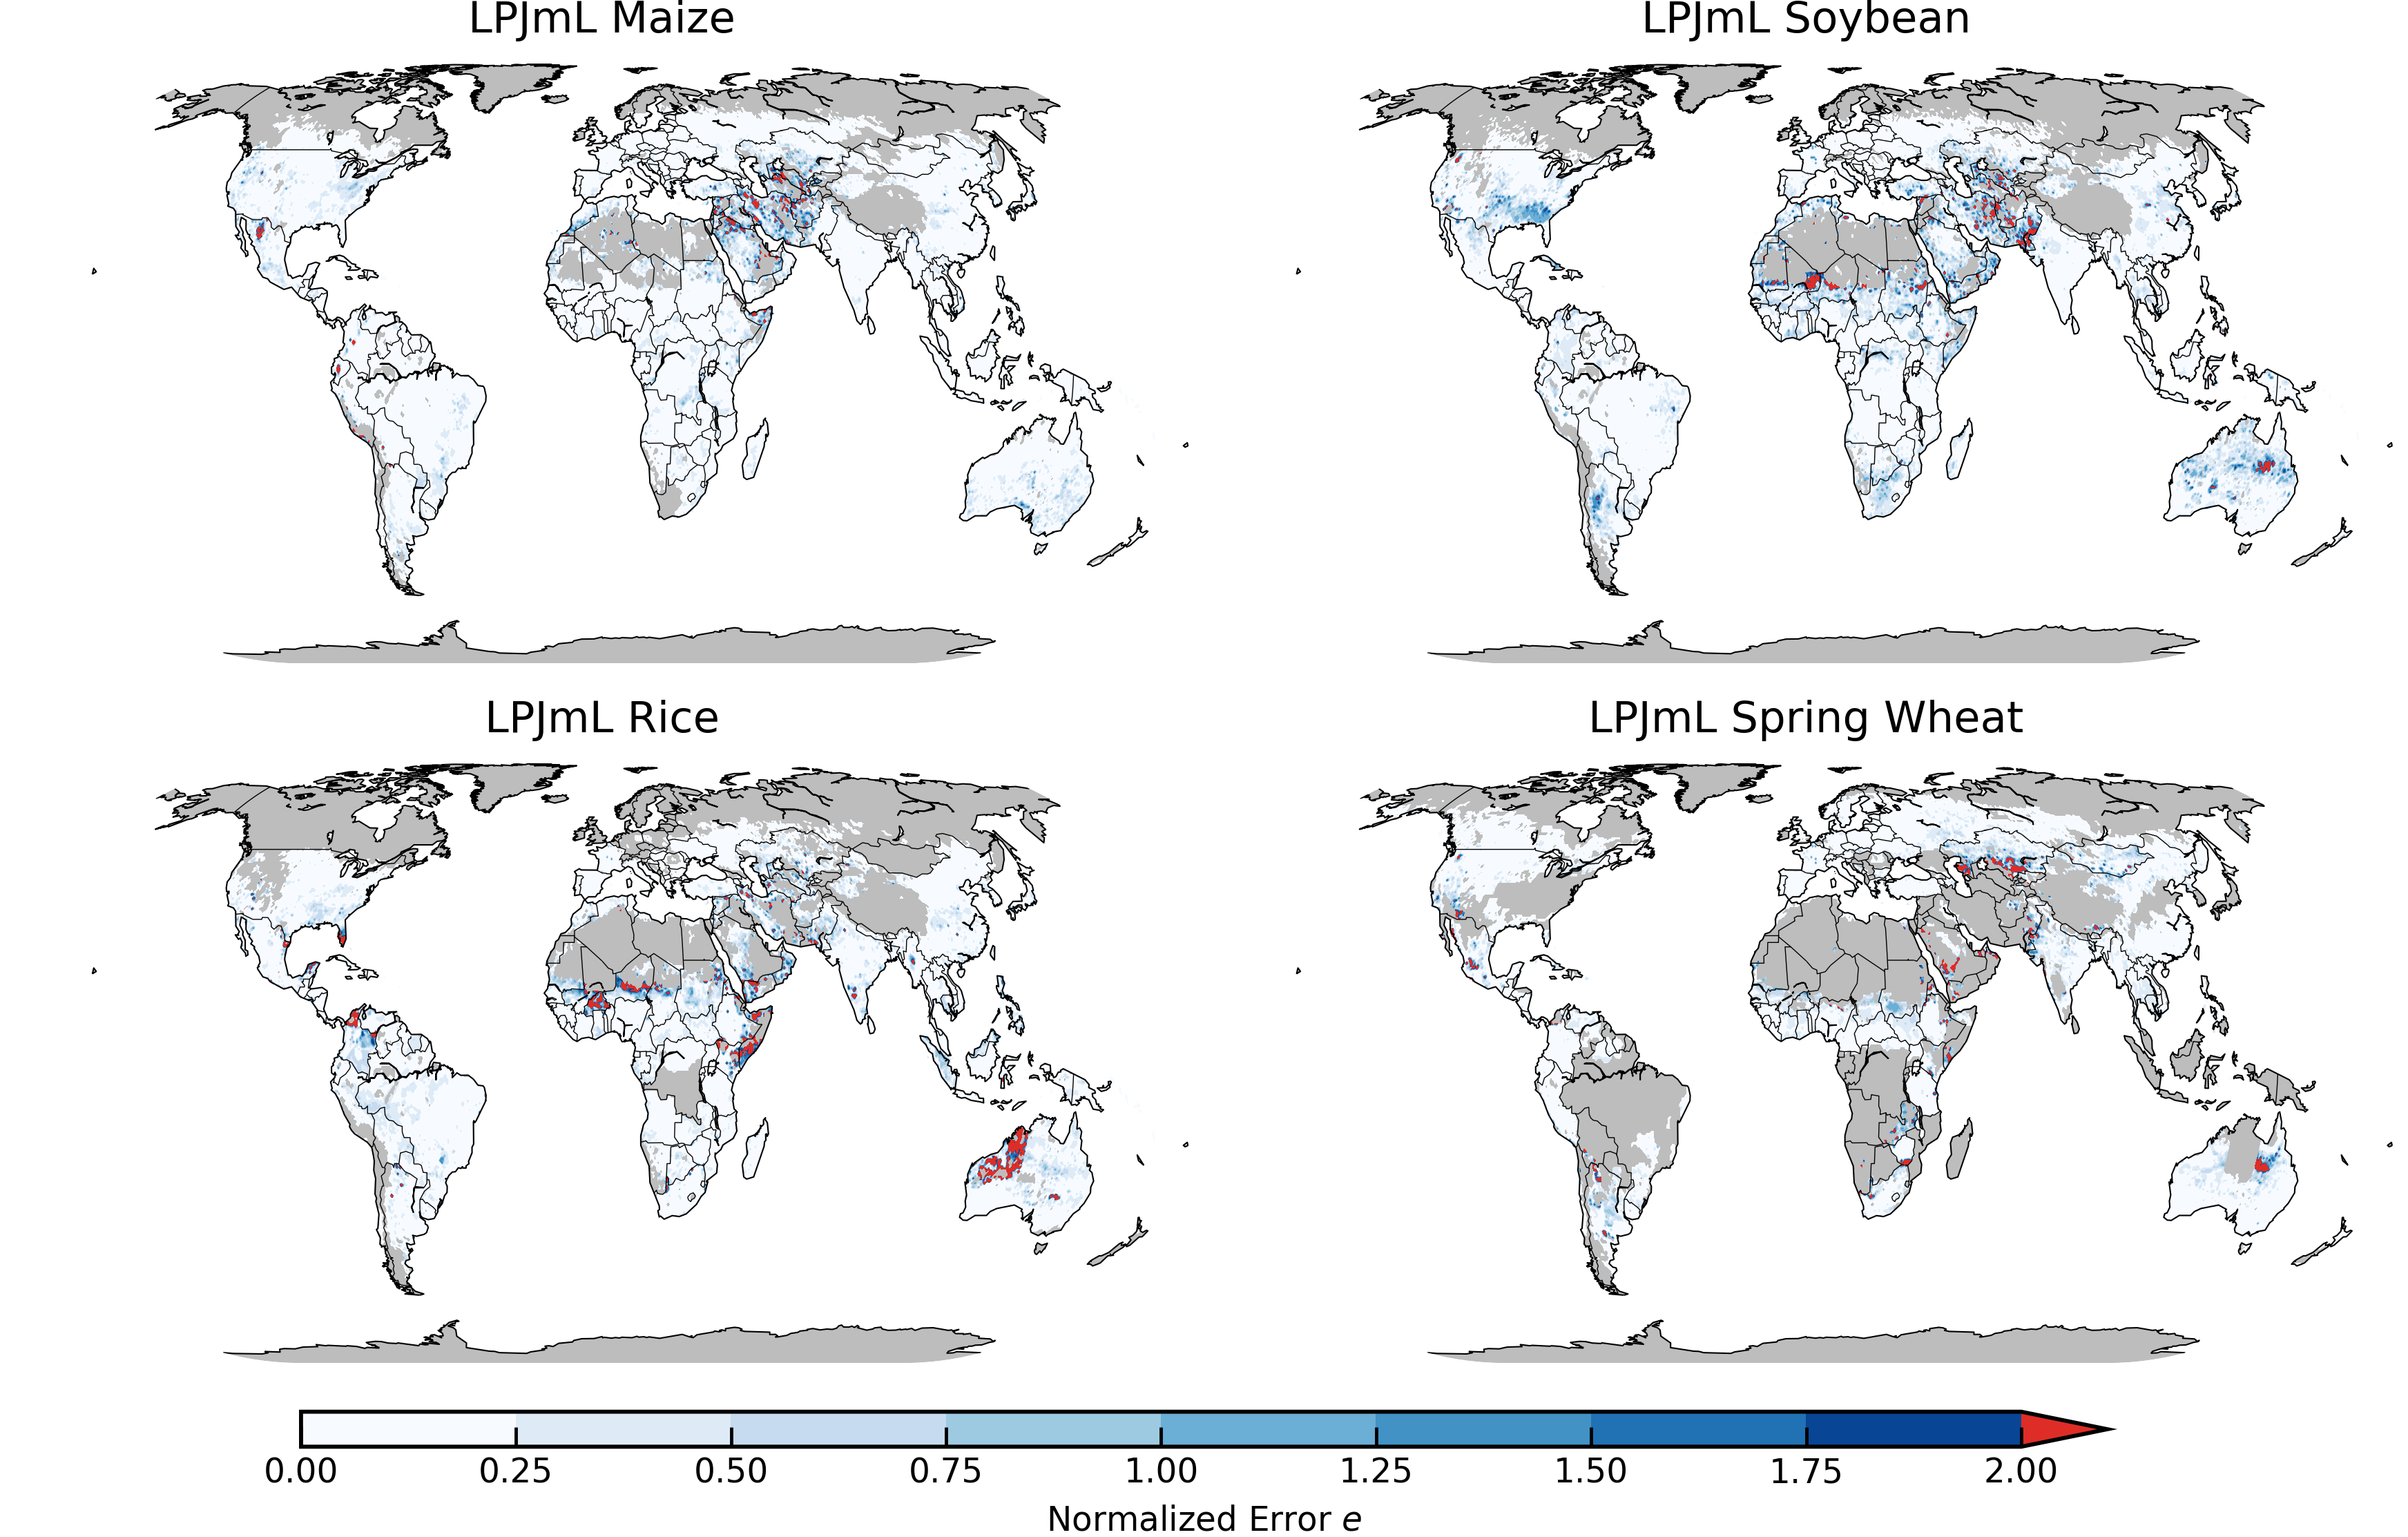
\includegraphics[width=15.5cm]{LPJmL_spatial_error.png}
\caption{Same convention as main text Figure 8 except now for LPJmL.}
\label{fig:lpjmlnorm}
\end{figure}

\begin{figure}[h!]
%S14
\centering
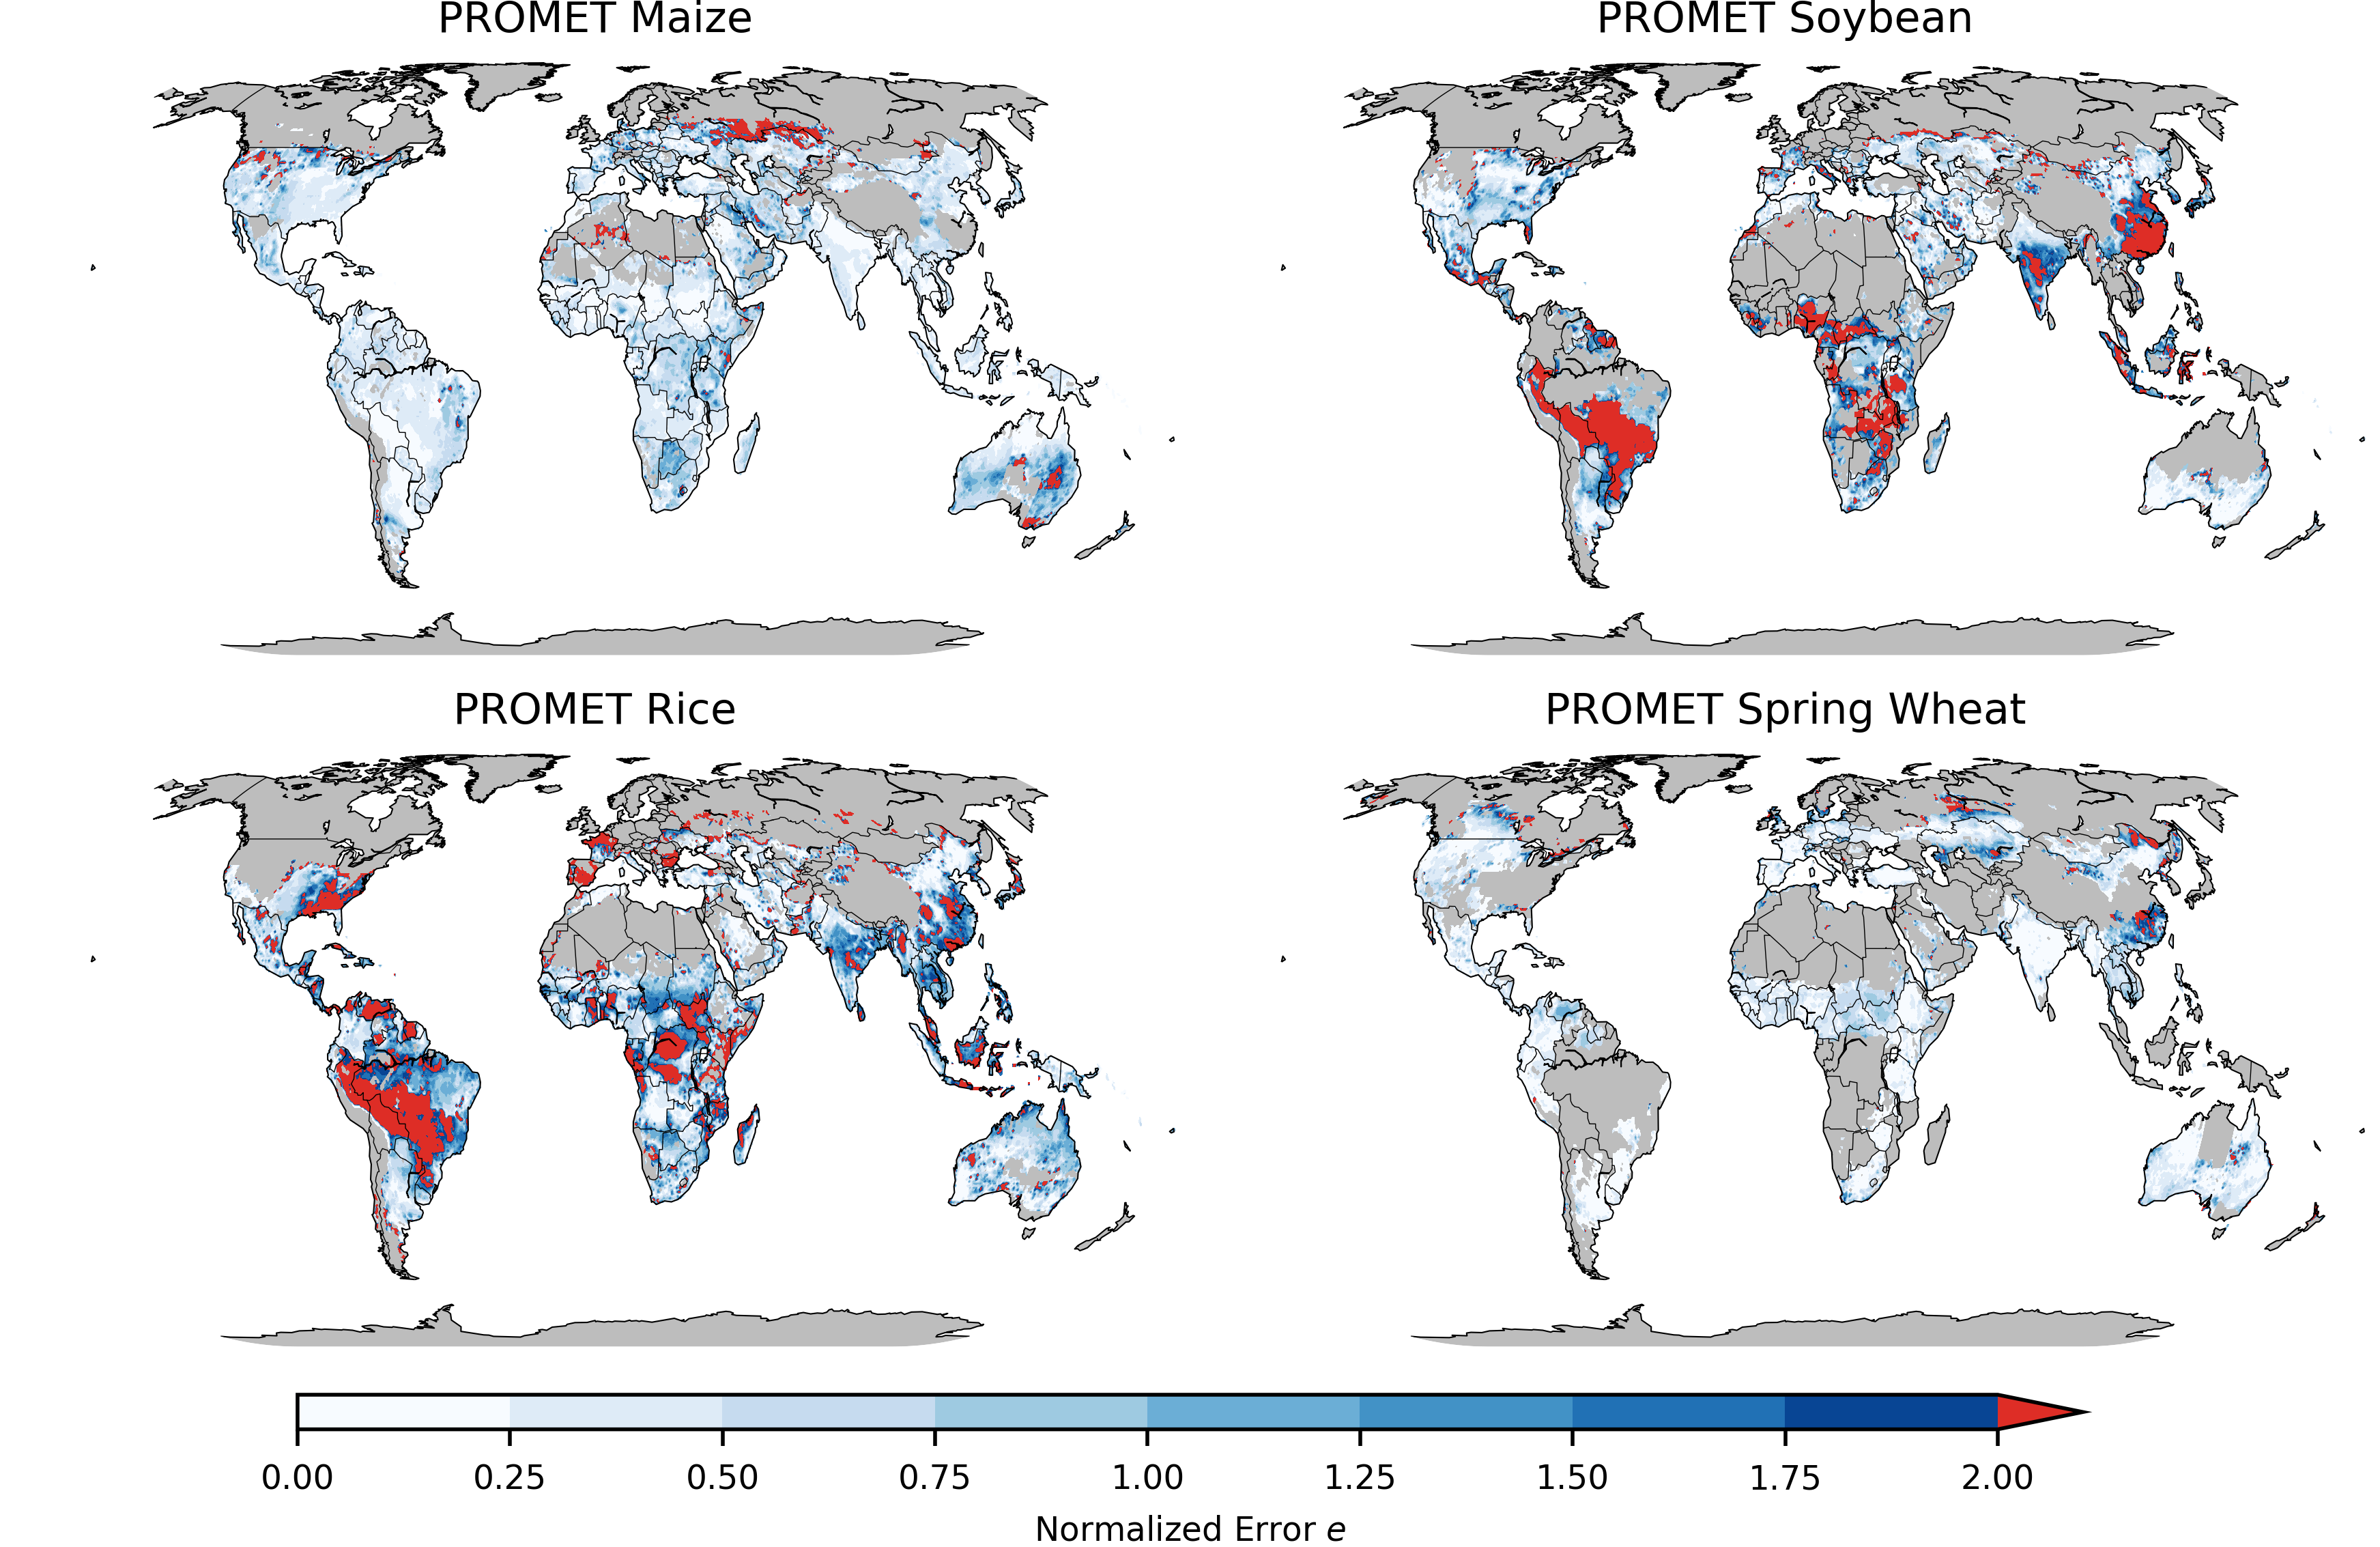
\includegraphics[width=15.5cm]{PROMET_spatial_error.png}
\caption{Same convention as main text Figure 8 except now for PROMET.}
\label{fig:lpjmlnorm}
\end{figure}

\begin{figure}[h!]
%S15
\centering
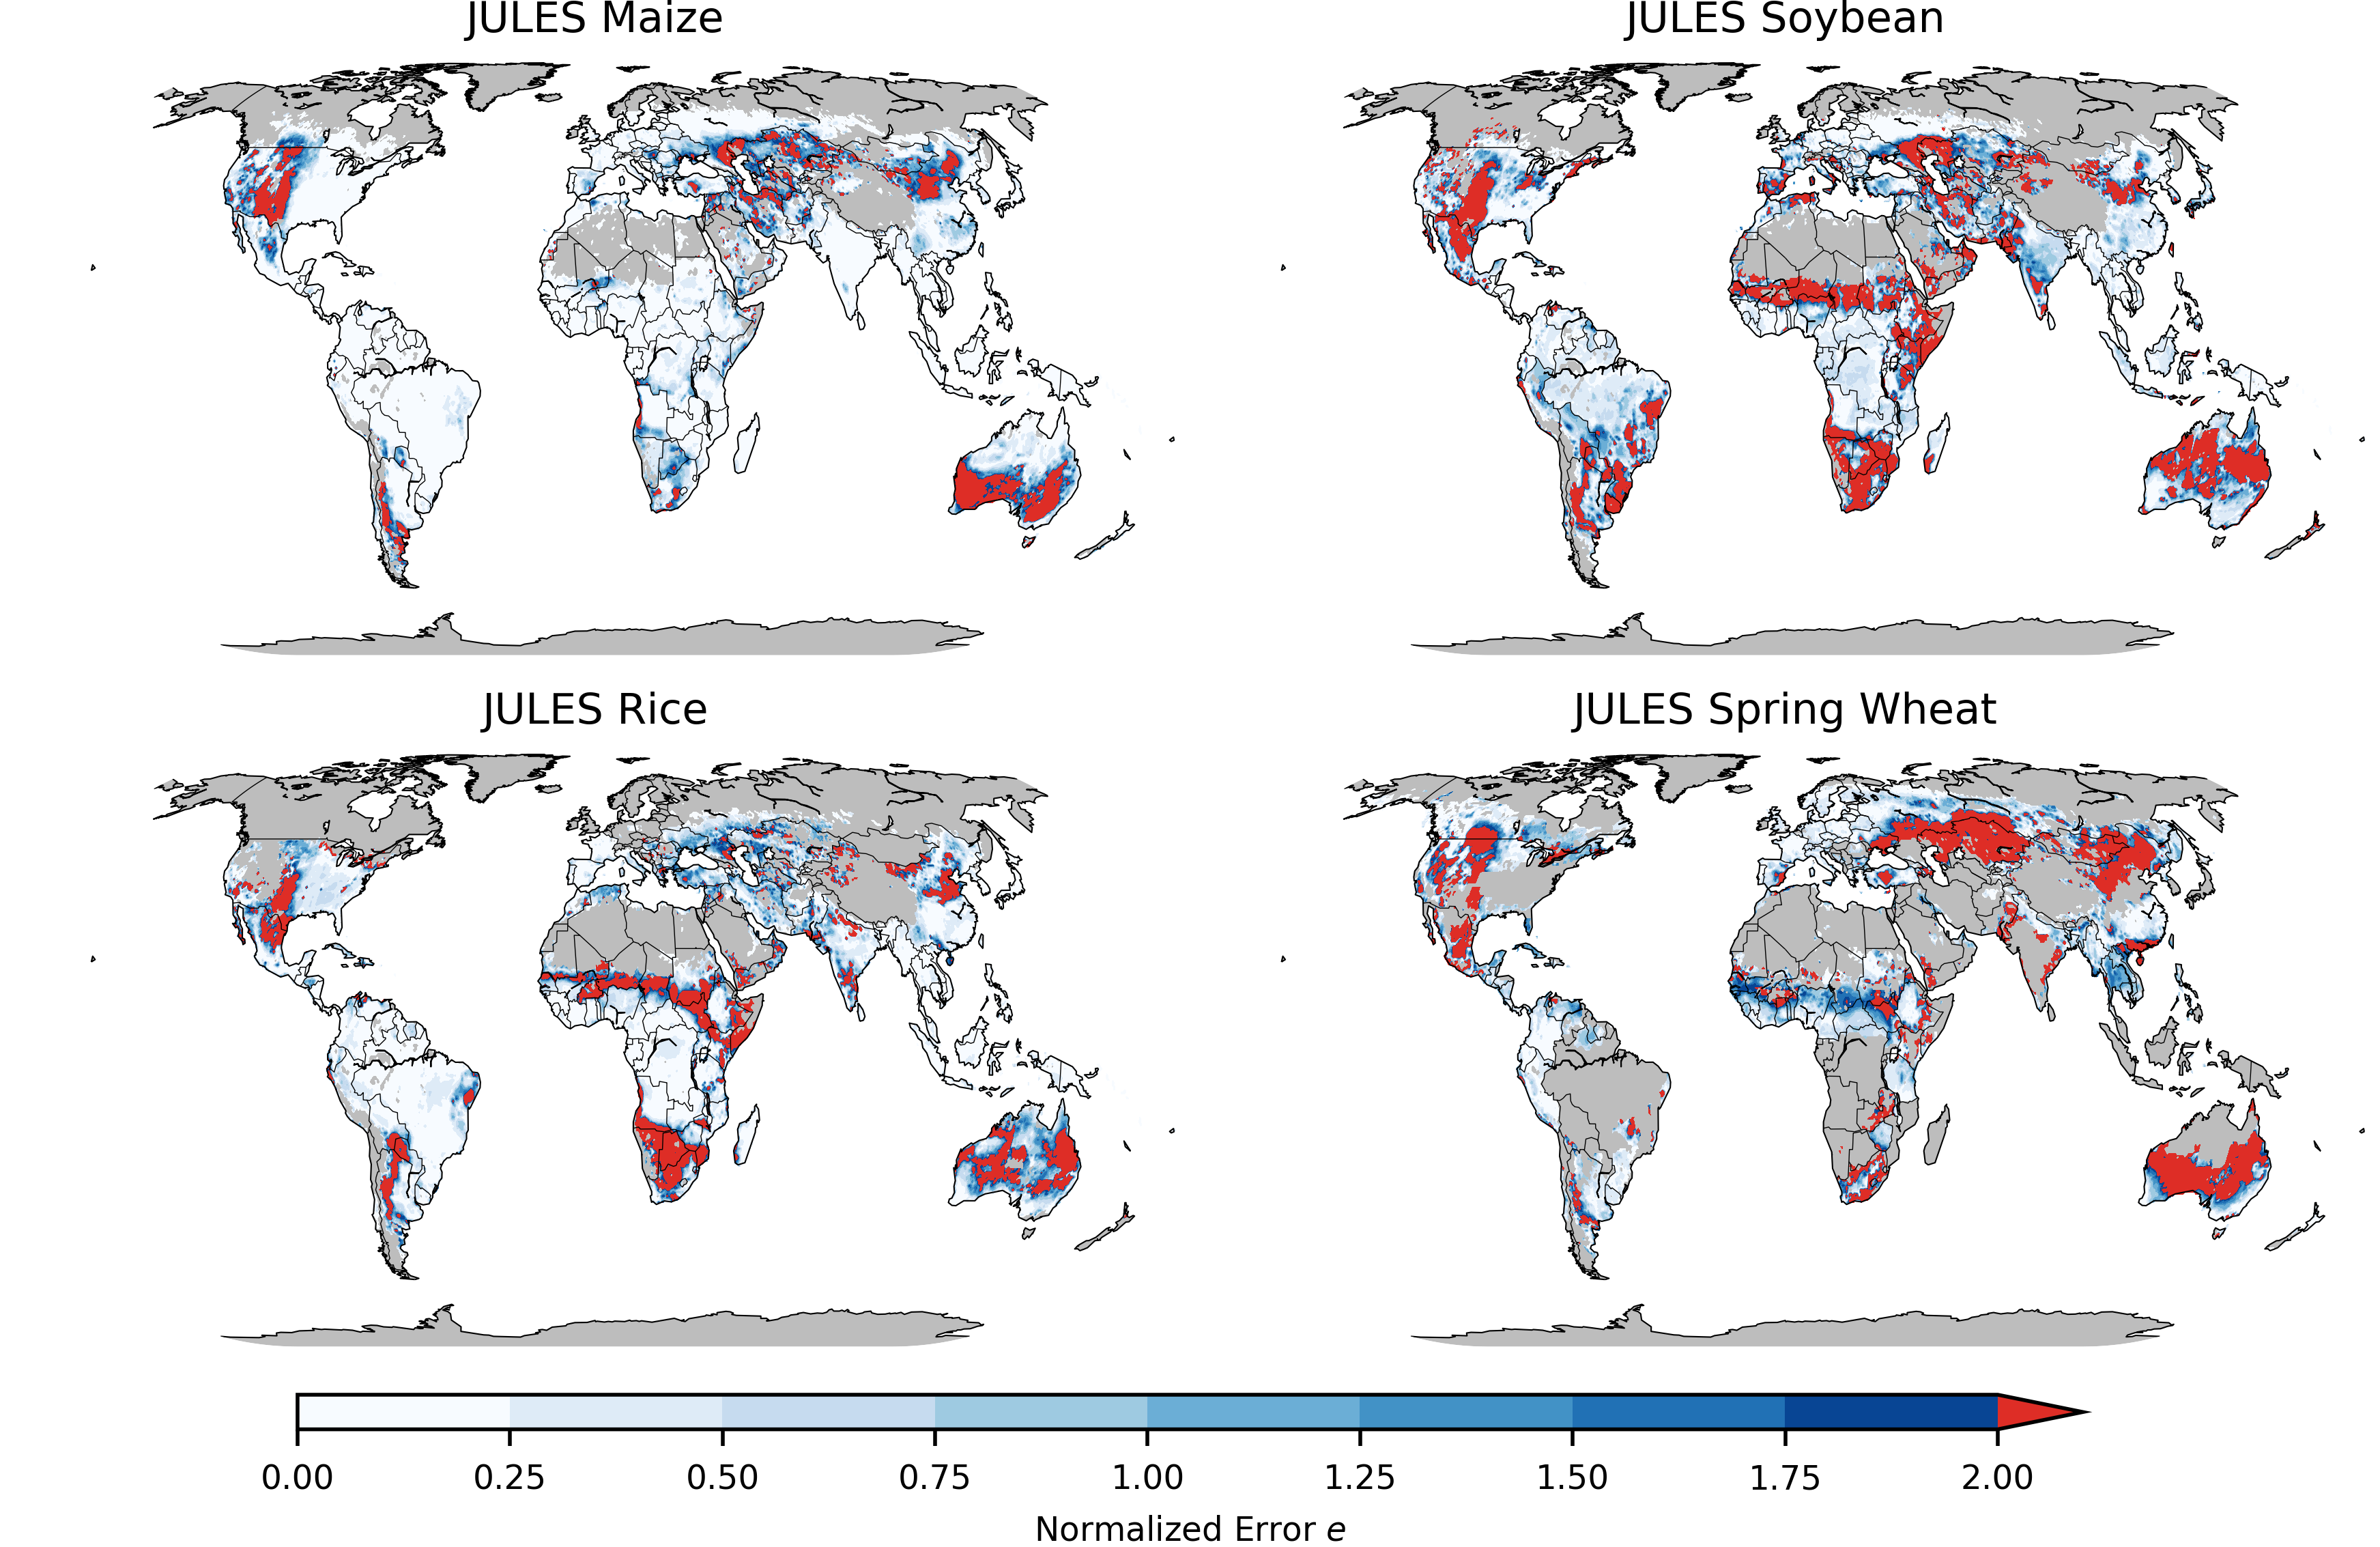
\includegraphics[width=15.5cm]{JULES_spatial_error.png}
\caption{Same convention as main text Figure 8 except now for JULES.}
\label{fig:lpjmlnorm}
\end{figure}

\begin{figure}[h!]
%S16
\centering
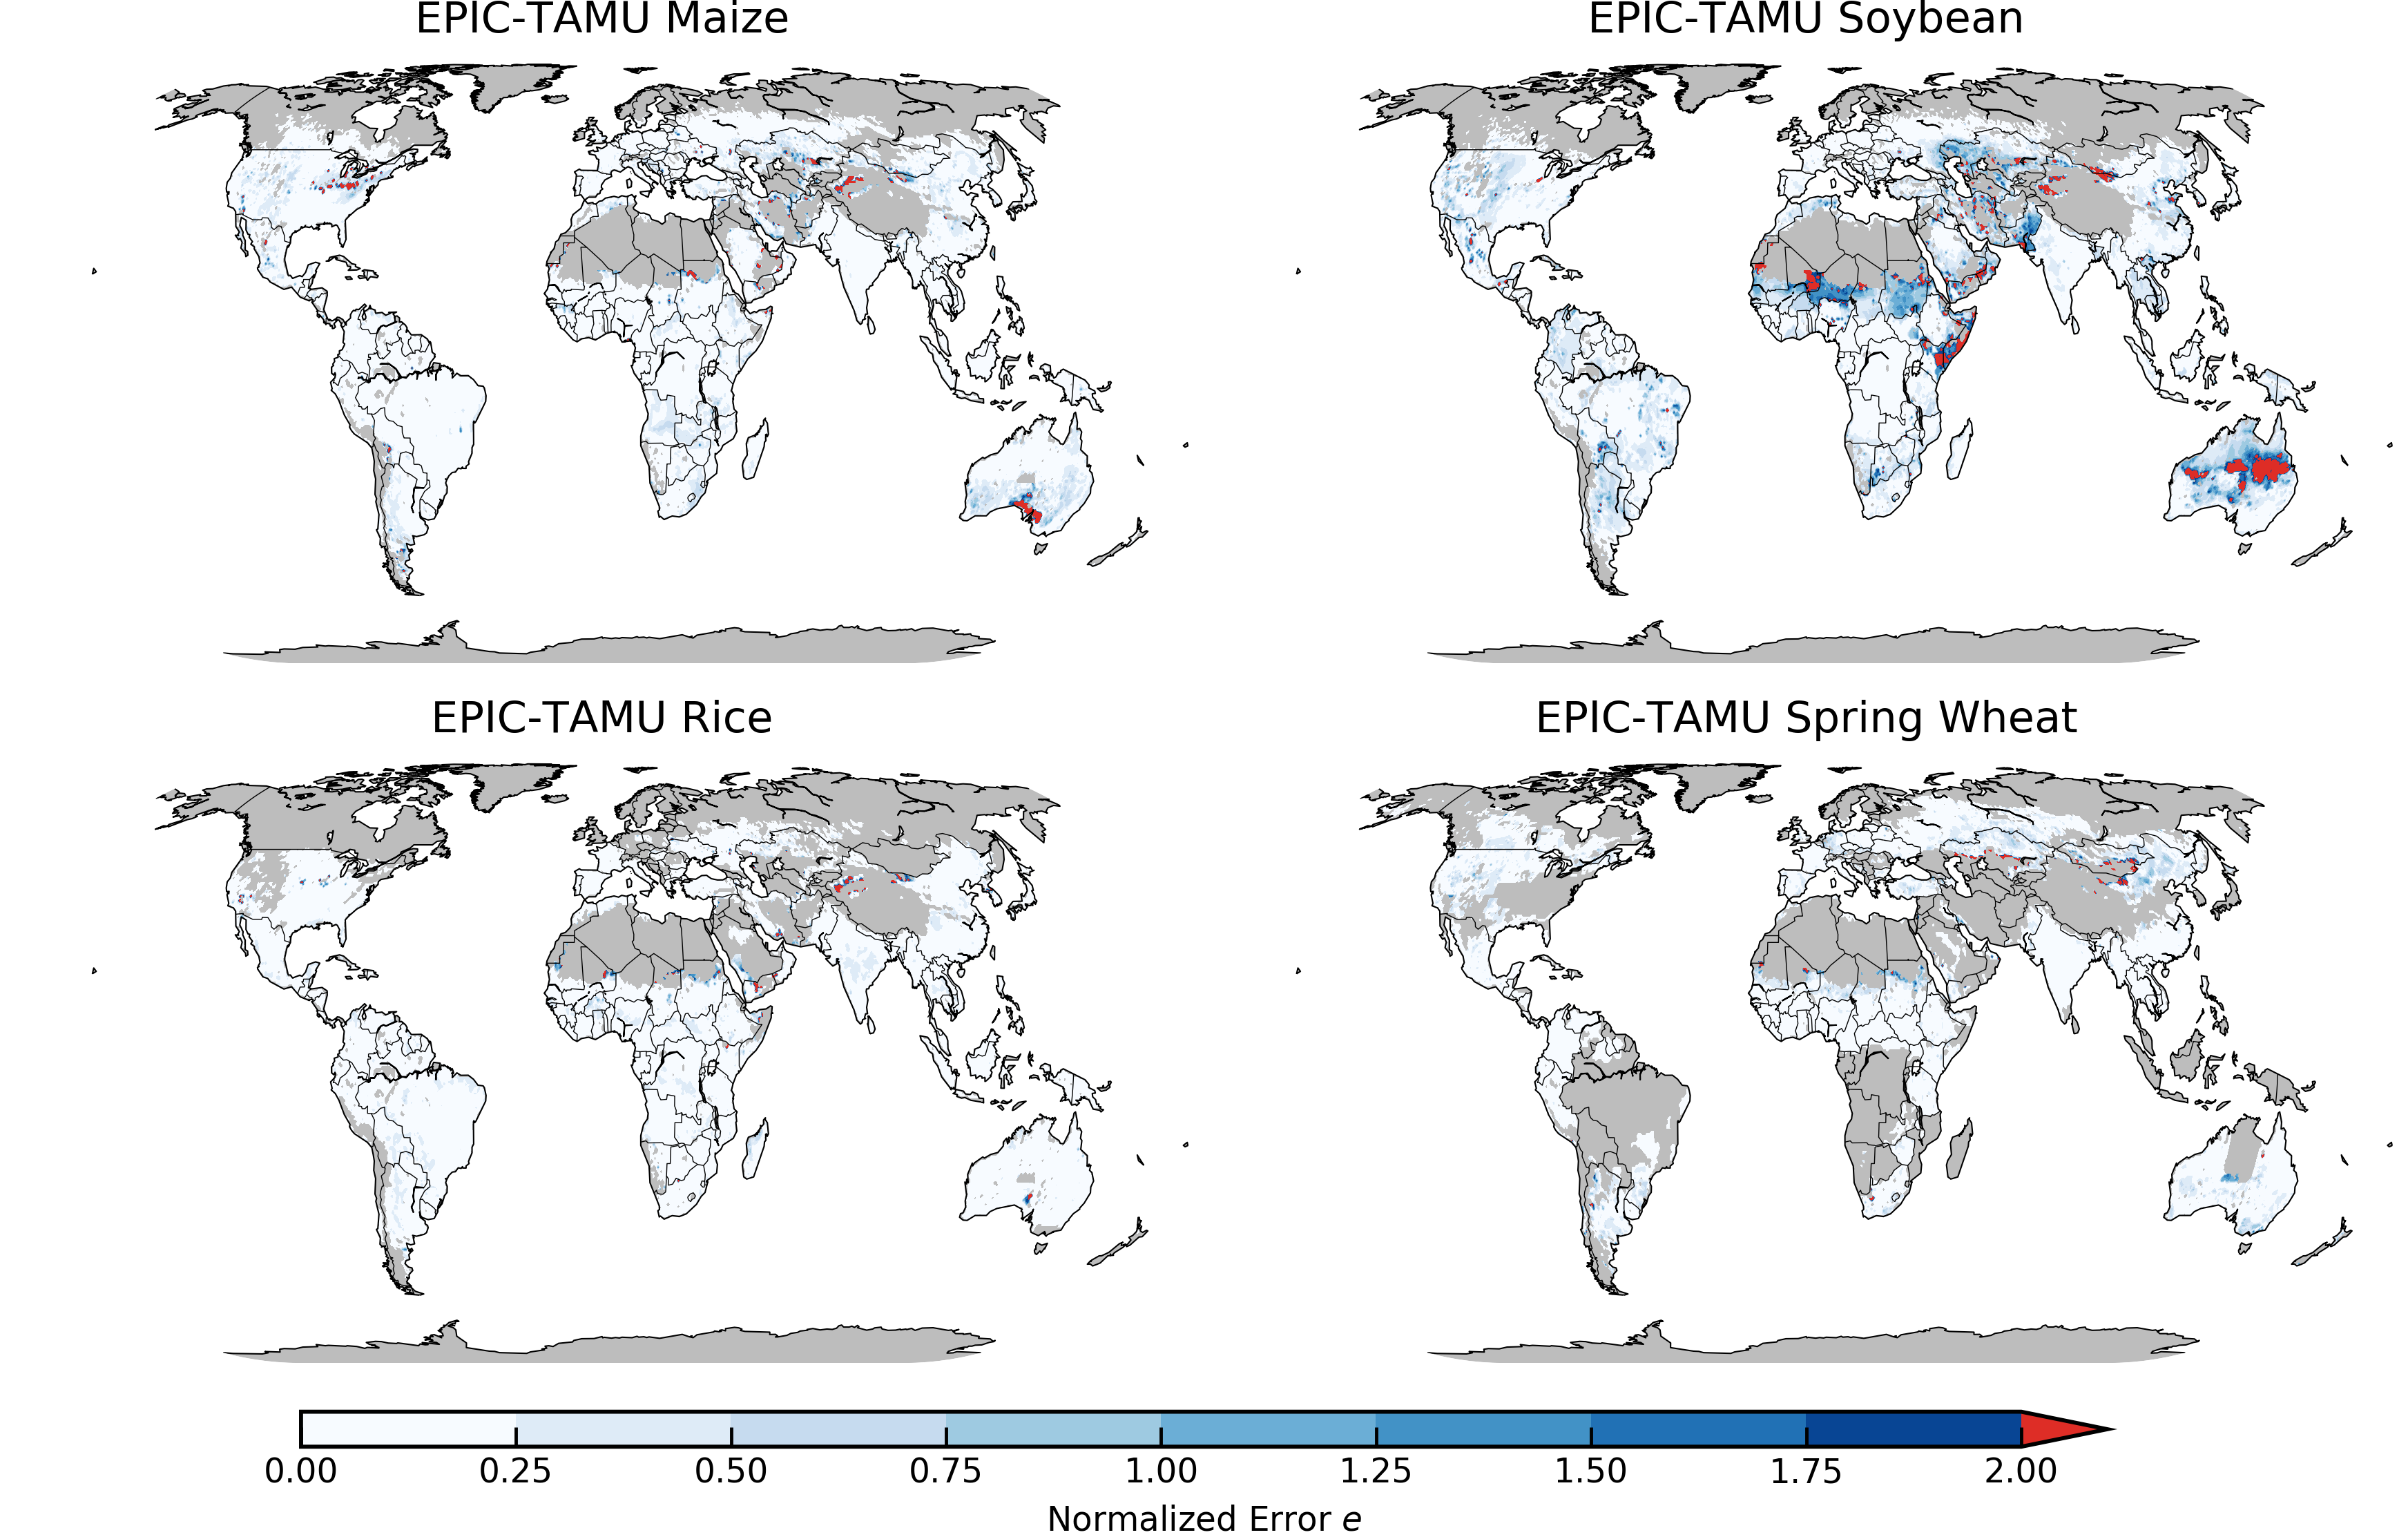
\includegraphics[width=15.5cm]{EPIC-TAMU_spatial_error.png}
\caption{Same convention as main text Figure 8 except now for EPIC-TAMU.}
\label{fig:lpjmlnorm}
\end{figure}

\begin{figure}[h!]
%S17
\centering
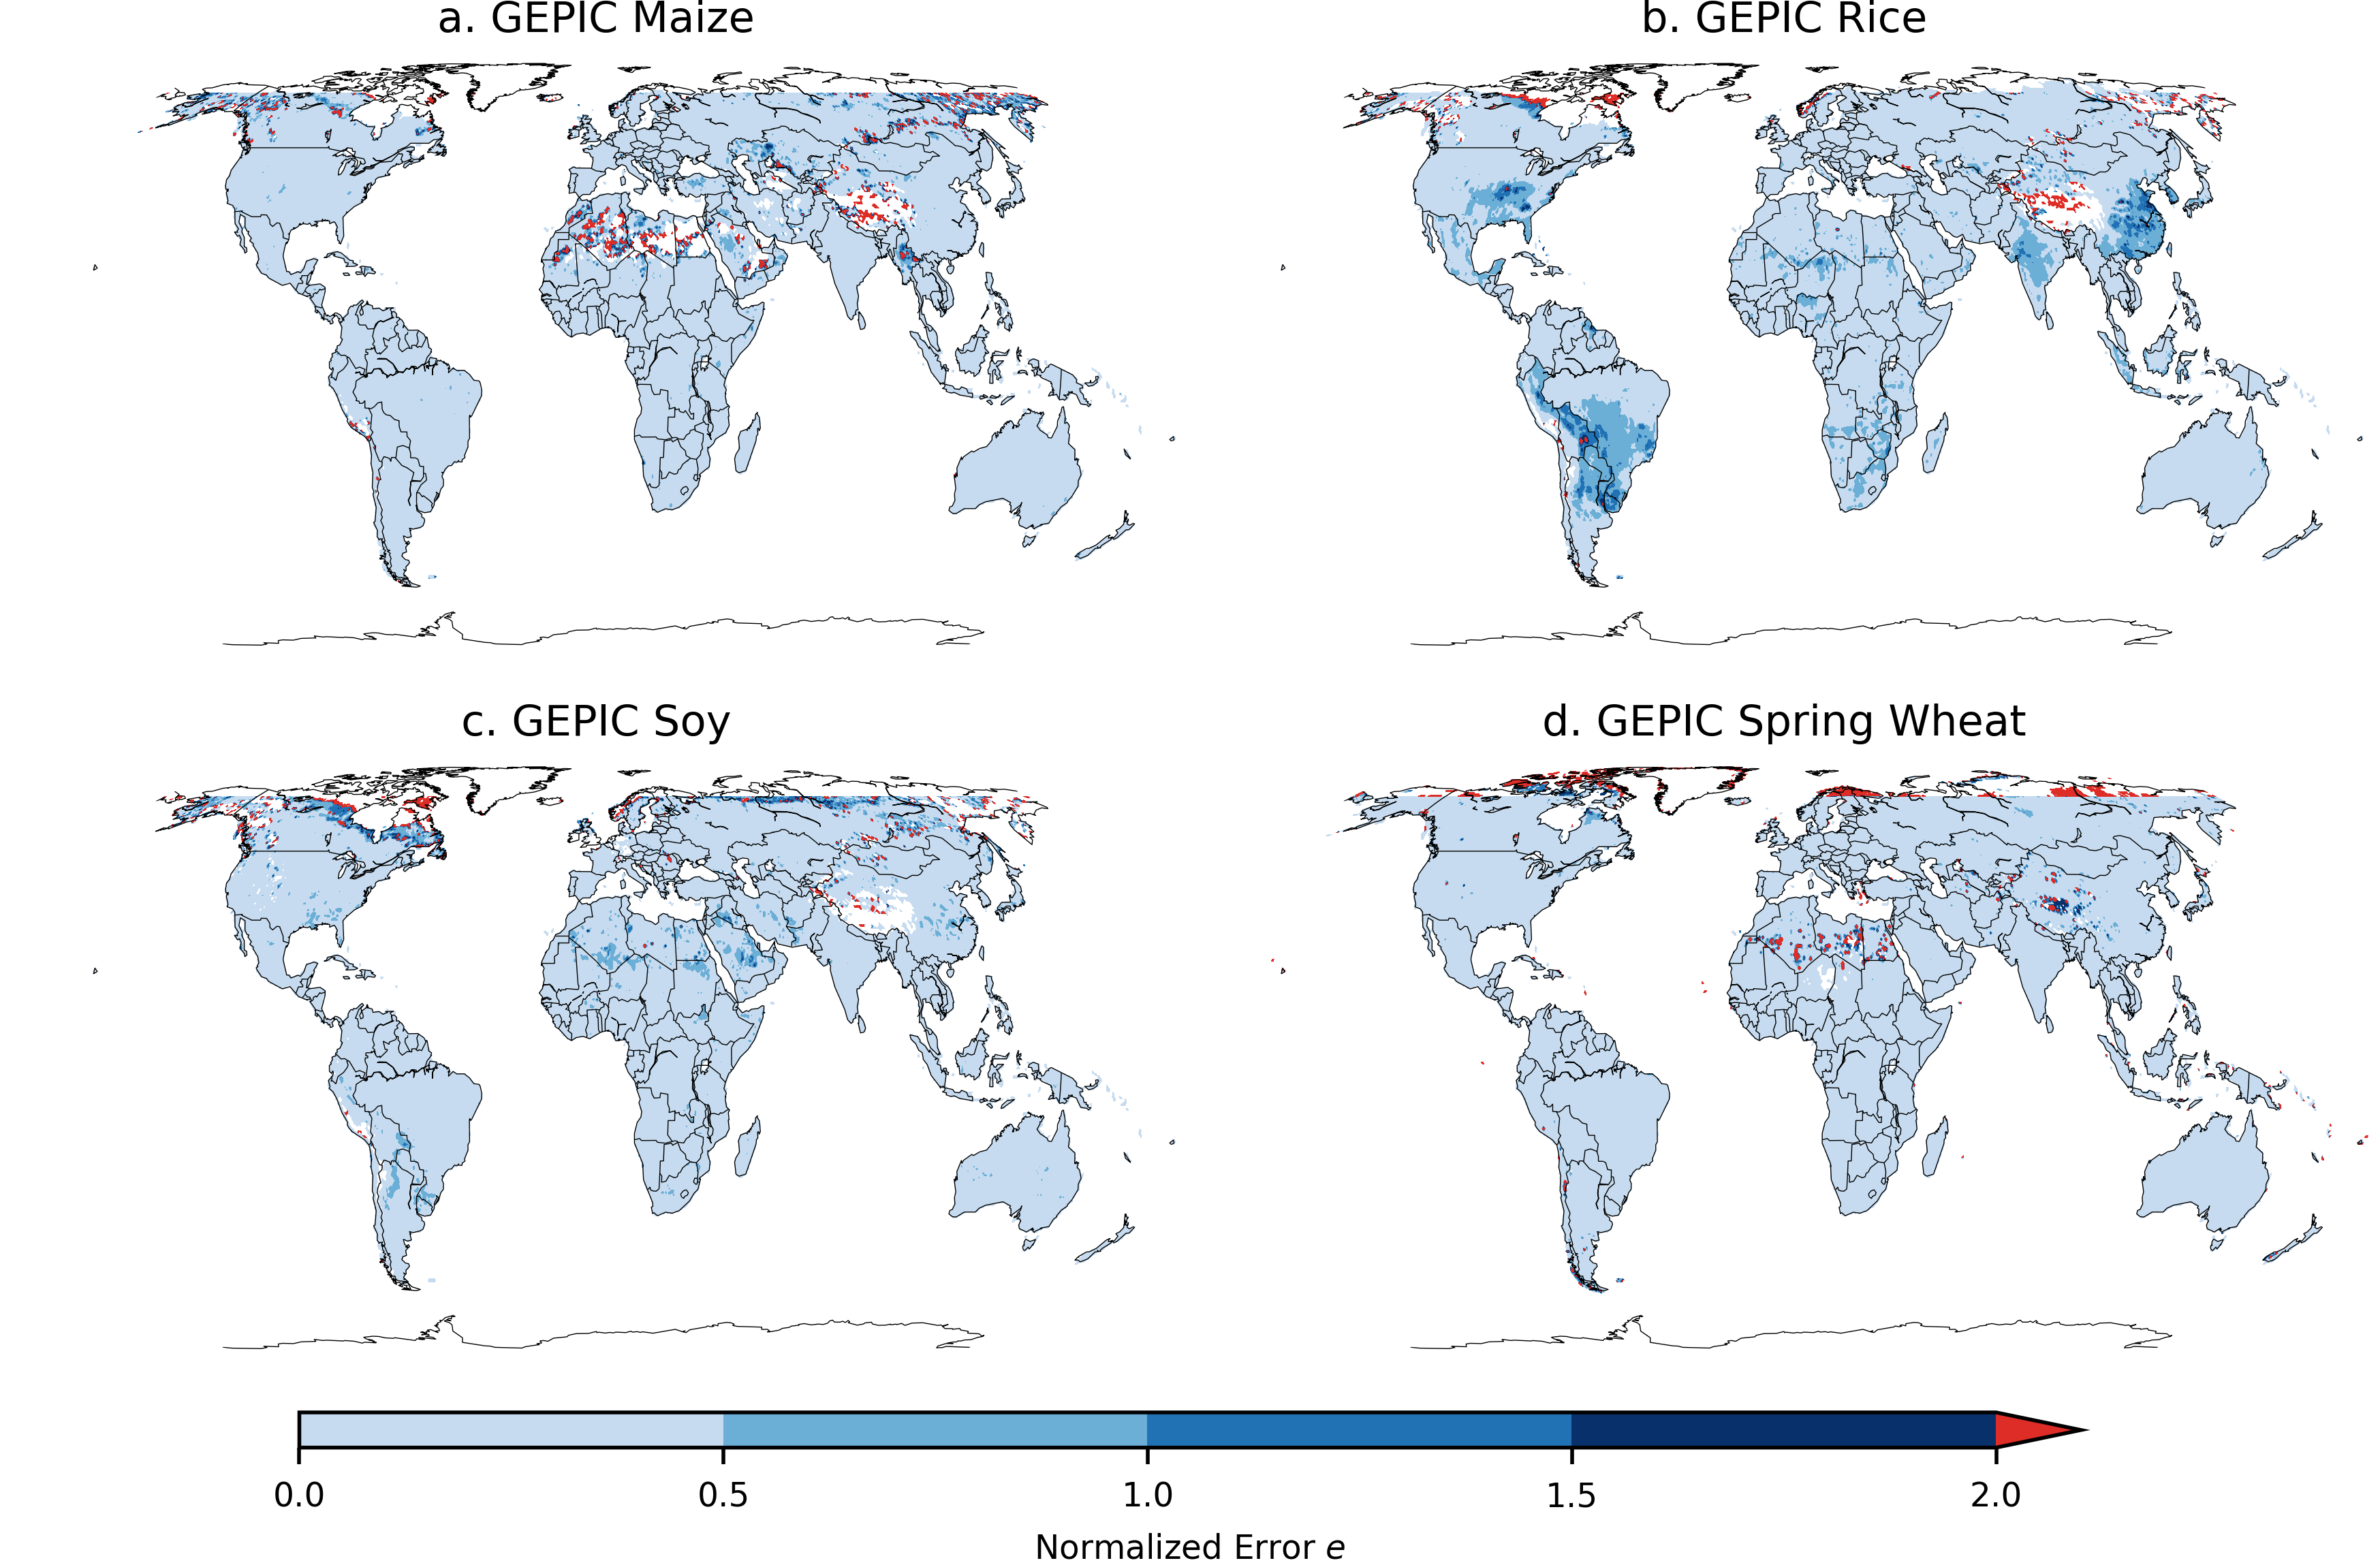
\includegraphics[width=15.5cm]{GEPIC_spatial_error.png}
\caption{Same convention as main text Figure 8 except now for GEPIC.}
\label{fig:lpjmlnorm}
\end{figure}

\begin{figure}[h!]
%S18
\centering
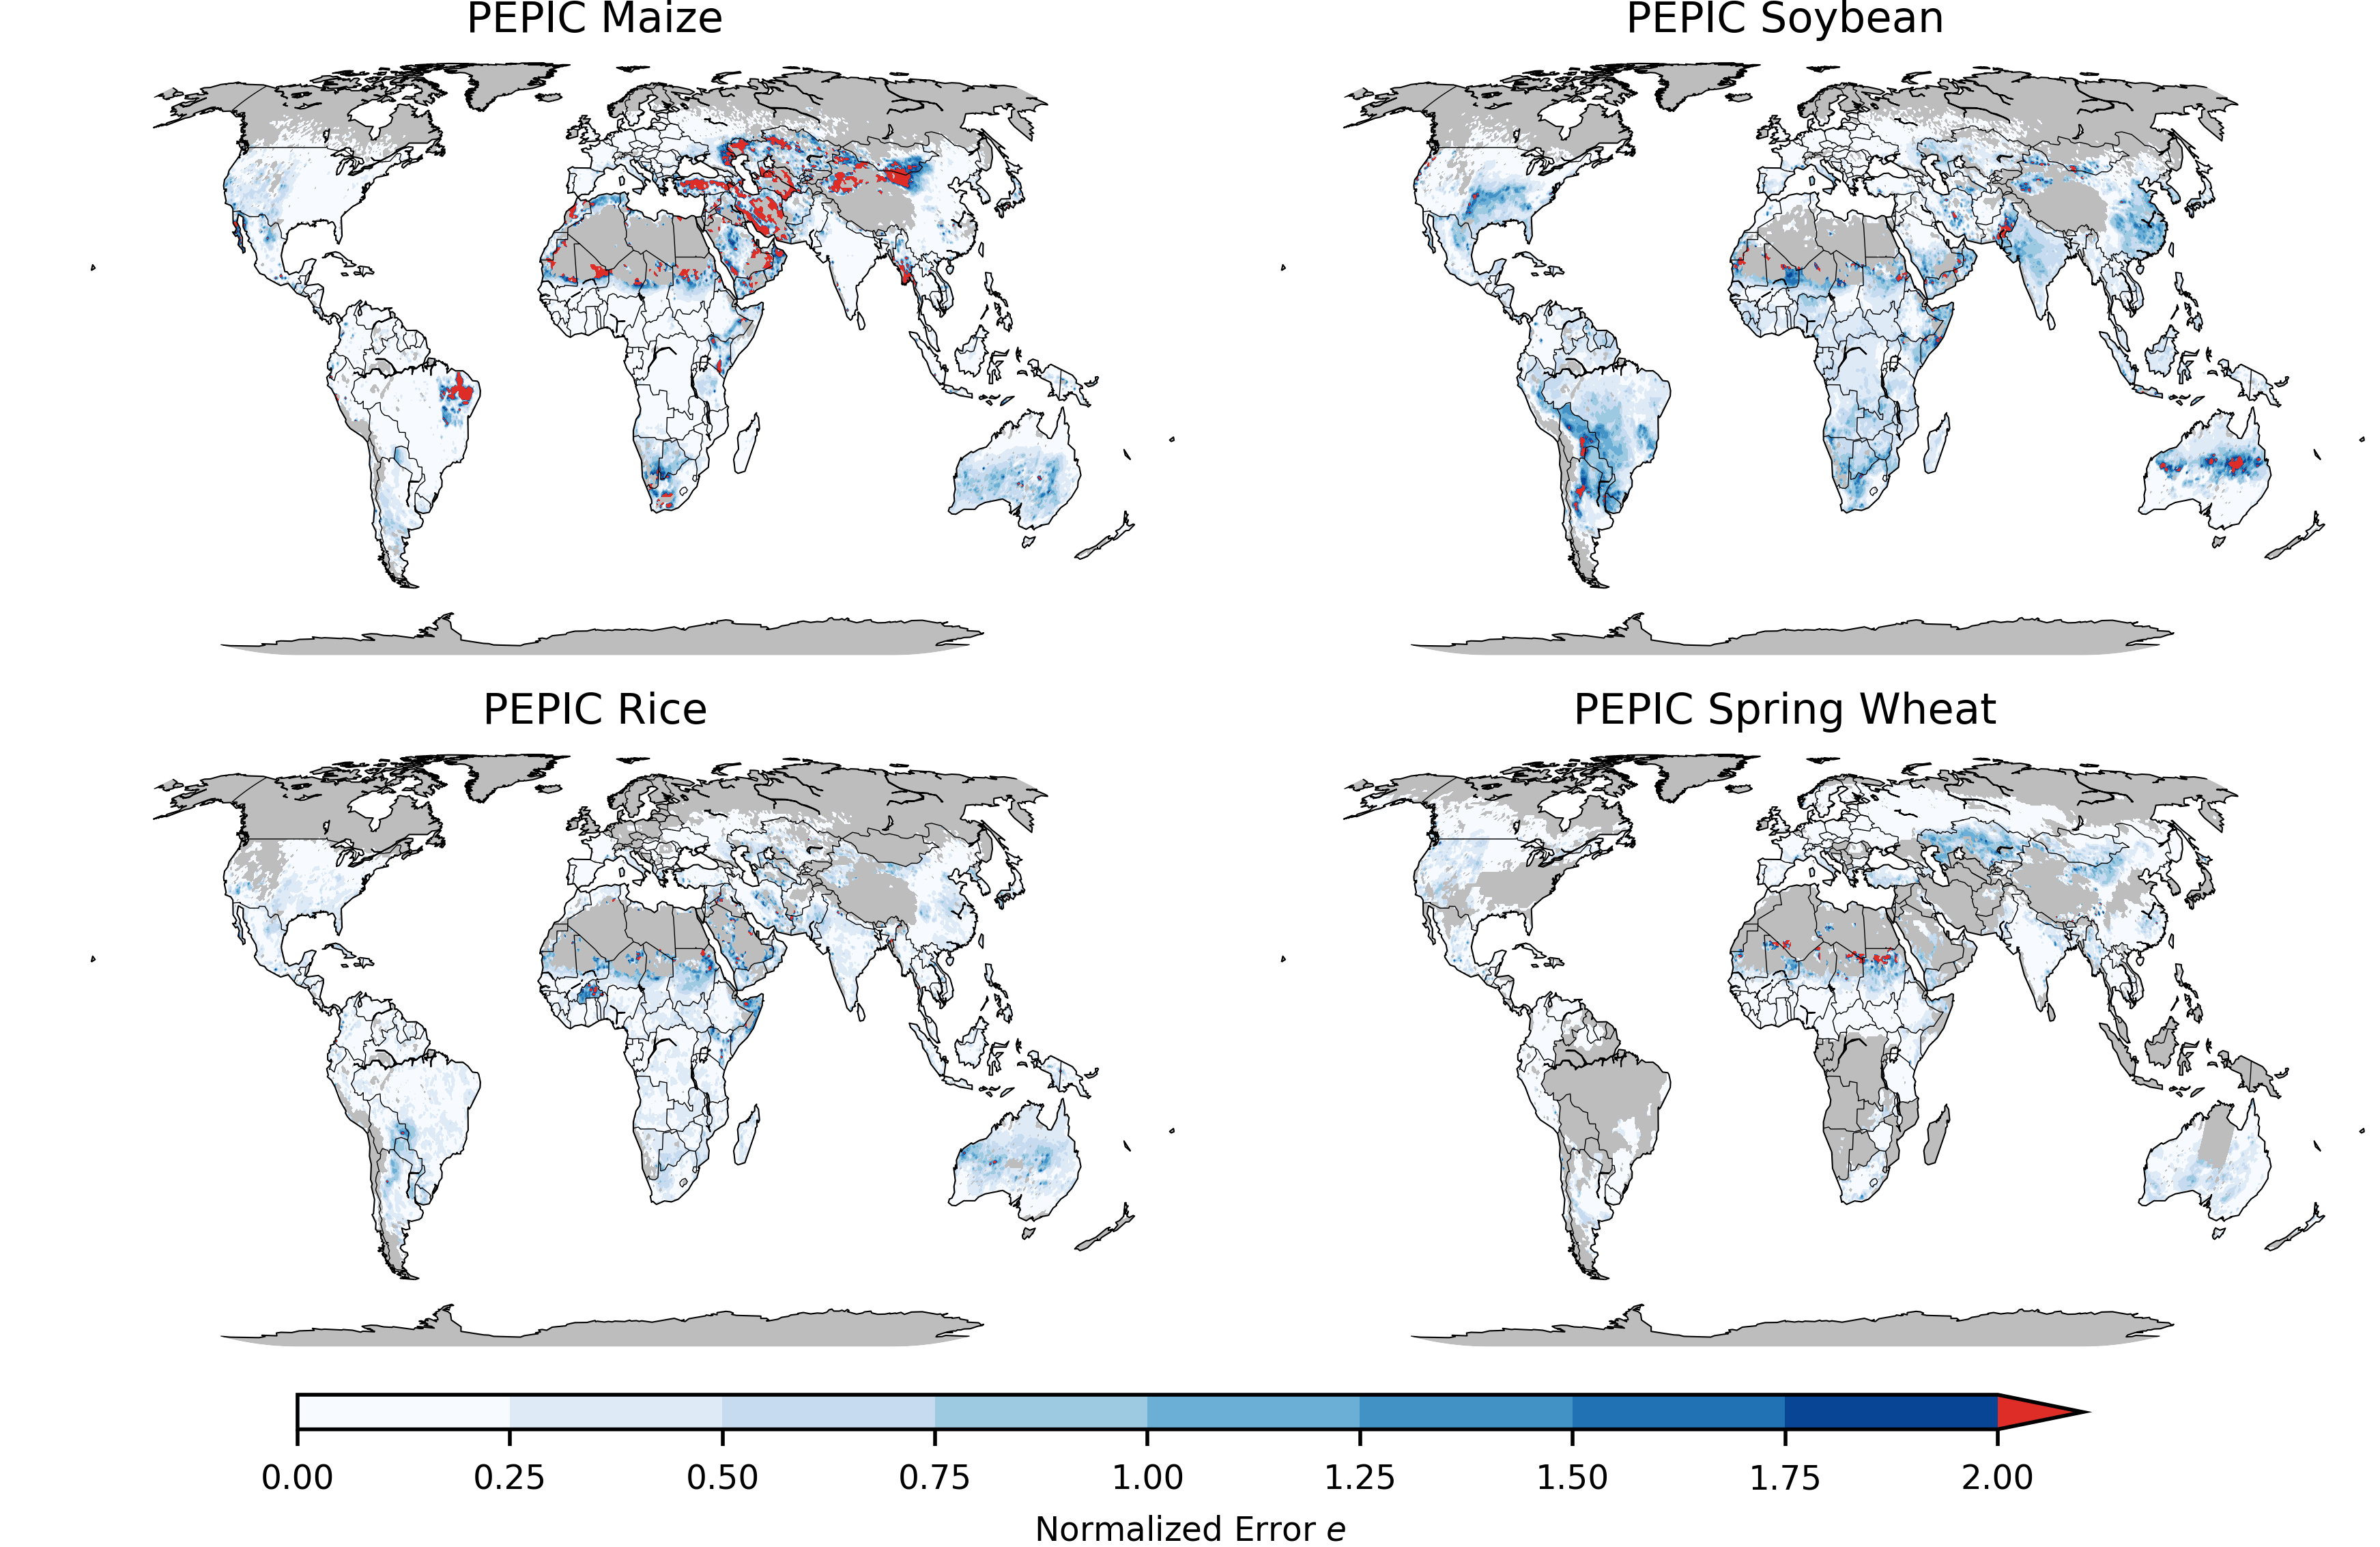
\includegraphics[width=15.5cm]{PEPIC_spatial_error.png}
\caption{Same convention as main text Figure 8 except now for PEPIC.}
\label{fig:lpjmlnorm}
\end{figure}

%%%%%%%%%%%%%%%%%%%%%%%%%%%%%%%%%%%%%%%%%%%%%%%%%%%%%%%%%%%%%%%%%%%%%%%%%%%%%%%%%%%%%%%
%%%%%%%%%%%%%%%%%%%%%%%%%%%%%%%%%%%%%%%%%%%%%%%%%%%%%%%%%%%%%%%%%%%%%%%%%%%%%%%%%%%%%%%
%%%%%%%%%%%%%%%%%%%%%%%%%%%%%%%%%%%%%%%%%%%%%%%%%%%%%%%%%%%%%%%%%%%%%%%%%%%%%%%%%%%%%%%
\clearpage
\subsection{Cross Validation}

\begin{figure}[h!]
%S19
\centering
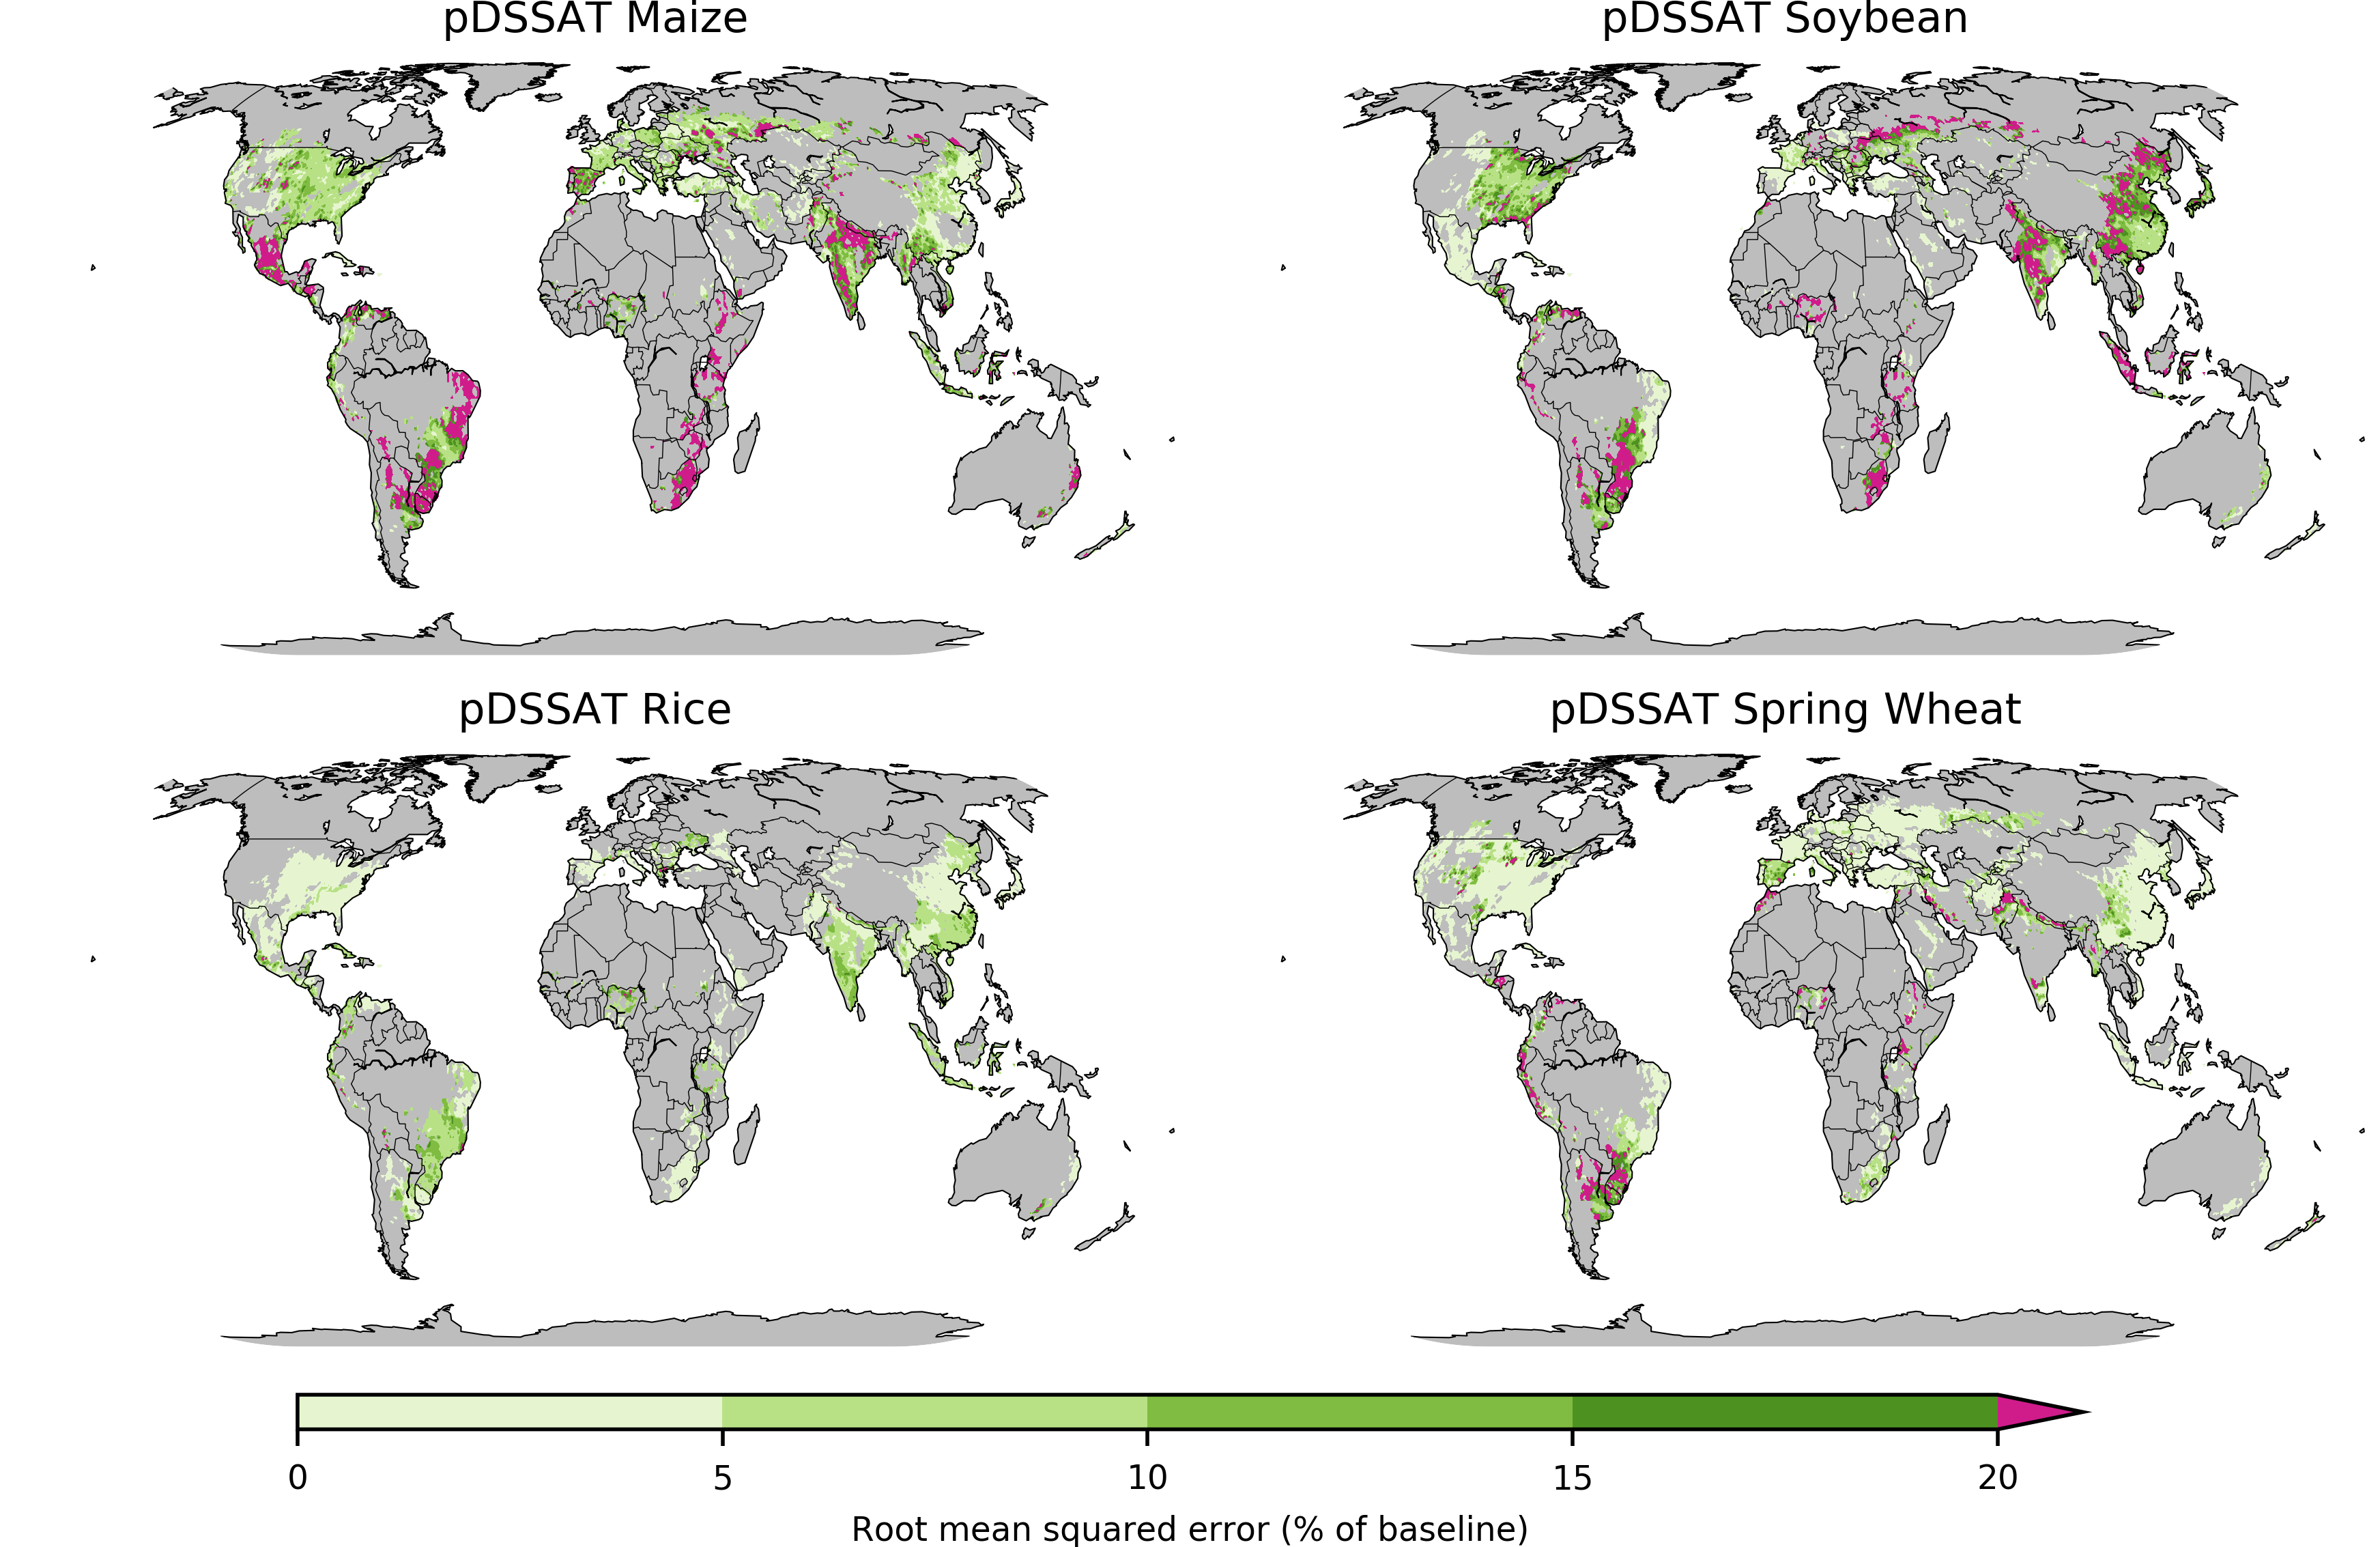
\includegraphics[width=15.5cm]{pDSSAT_spatial_MSE_ton_ha.png}
\caption{Root mean squared error for three fold cross validation process for the pDSSAT model for rainfed crops.}
\label{fig:pdssatrmse}
\end{figure}

\begin{figure}[h!]
%S20
\centering
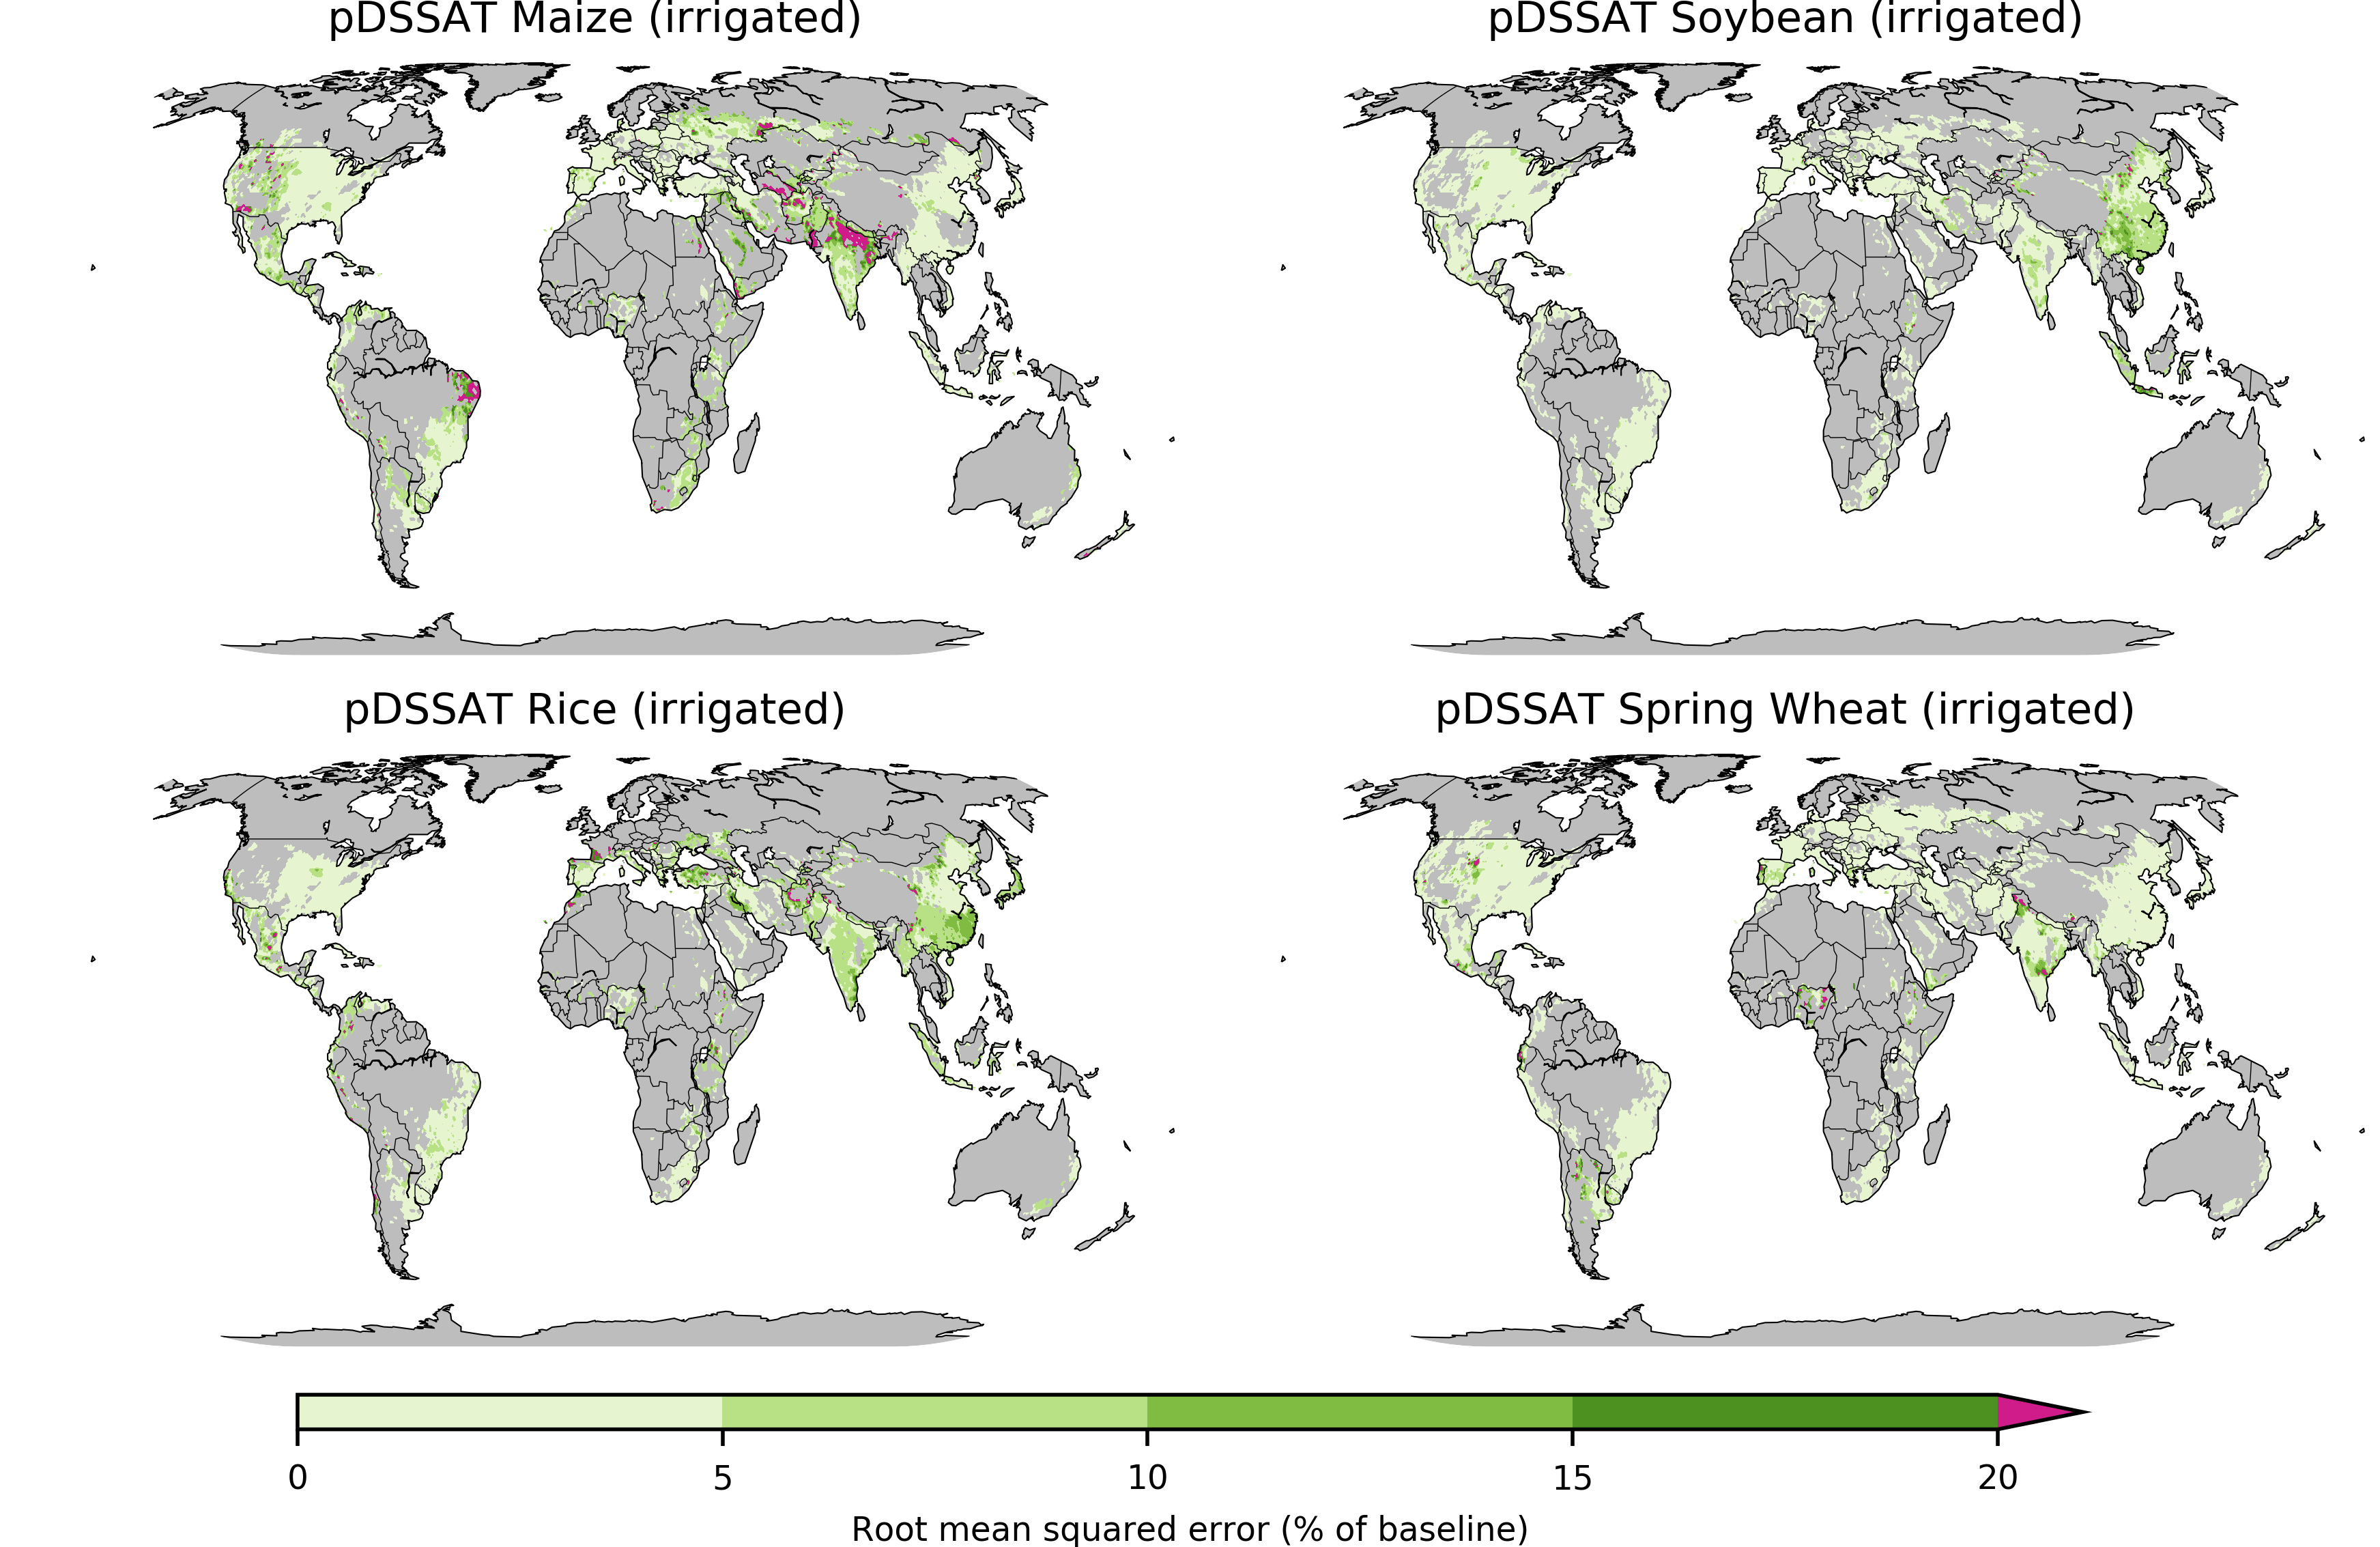
\includegraphics[width=15.5cm]{pDSSAT_spatial_MSE_ton_ha_irr.png}
\caption{Same as above for irrigated simulations.}
\label{fig:pdssatrmseirr}
\end{figure}

\begin{figure}[h!]
%S21
\centering
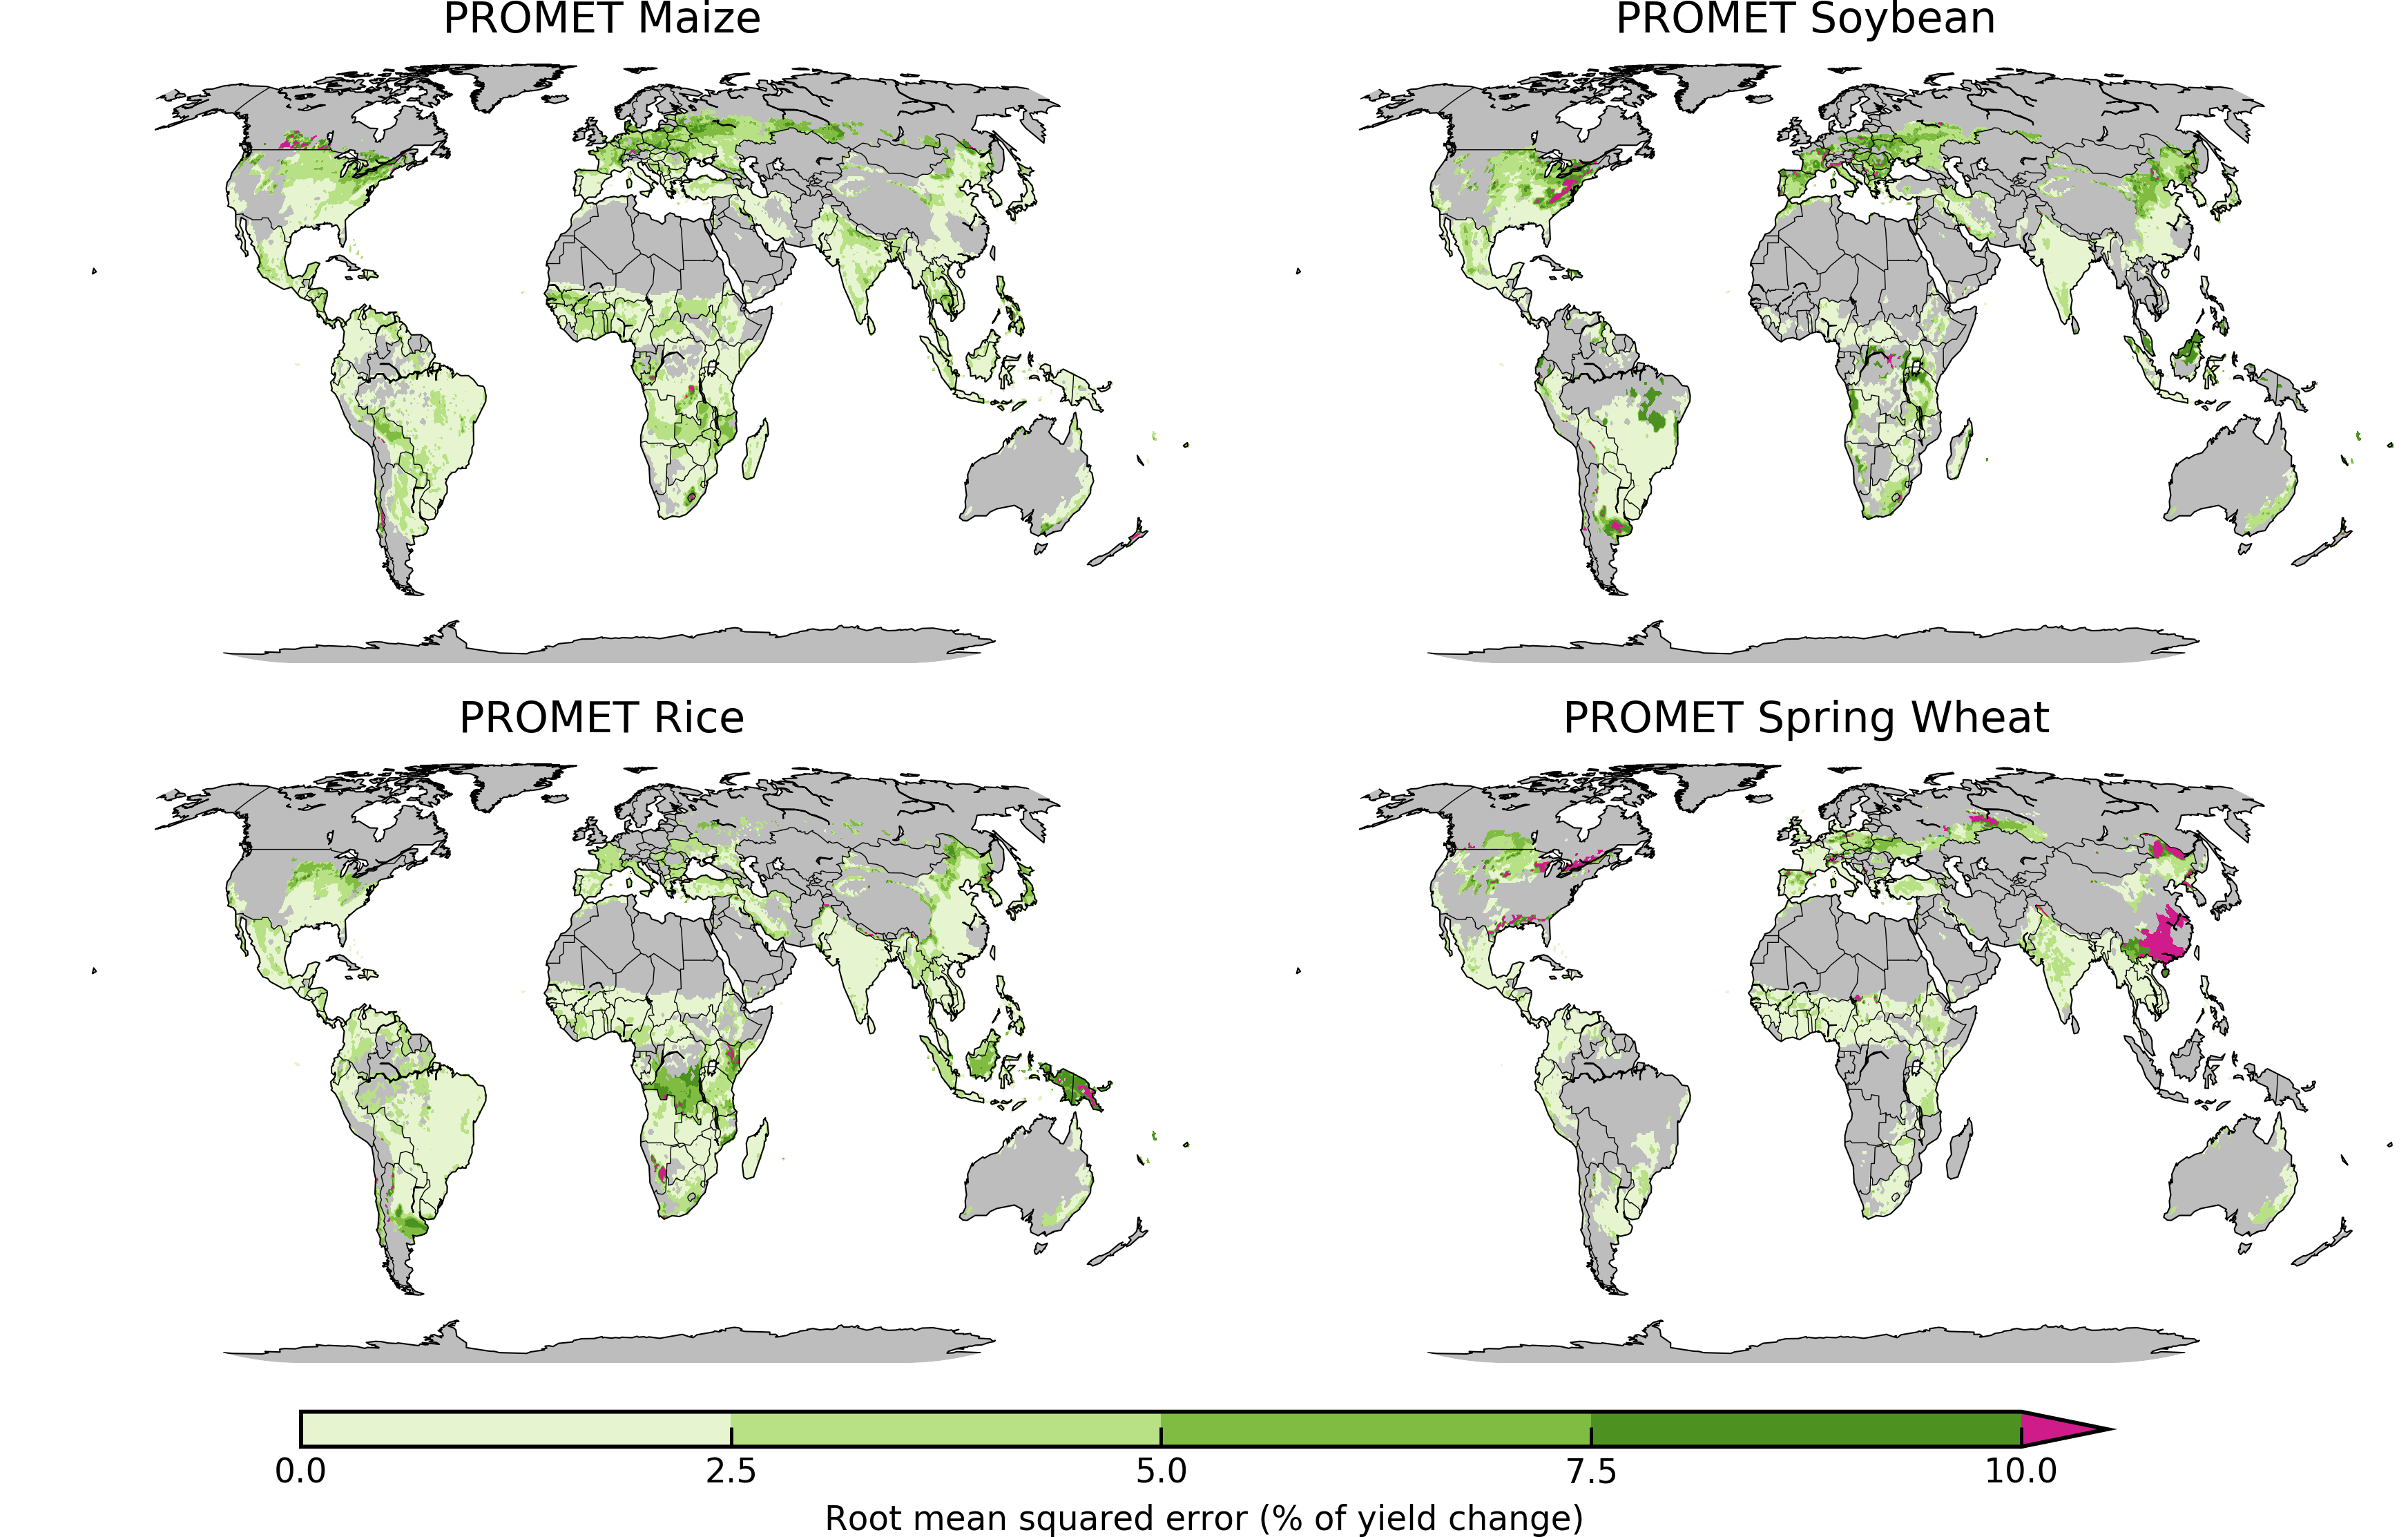
\includegraphics[width=15.5cm]{PROMET_spatial_MSE_ton_ha.png}
\caption{Map of root mean squared error for three fold cross validation process for the PROMET model for rainfed crops. Values shown as a percentage of baseline yield in each gridcell.}
\label{fig:pdssatrmse}
\end{figure}

\begin{figure}[h!]
%S22
\centering
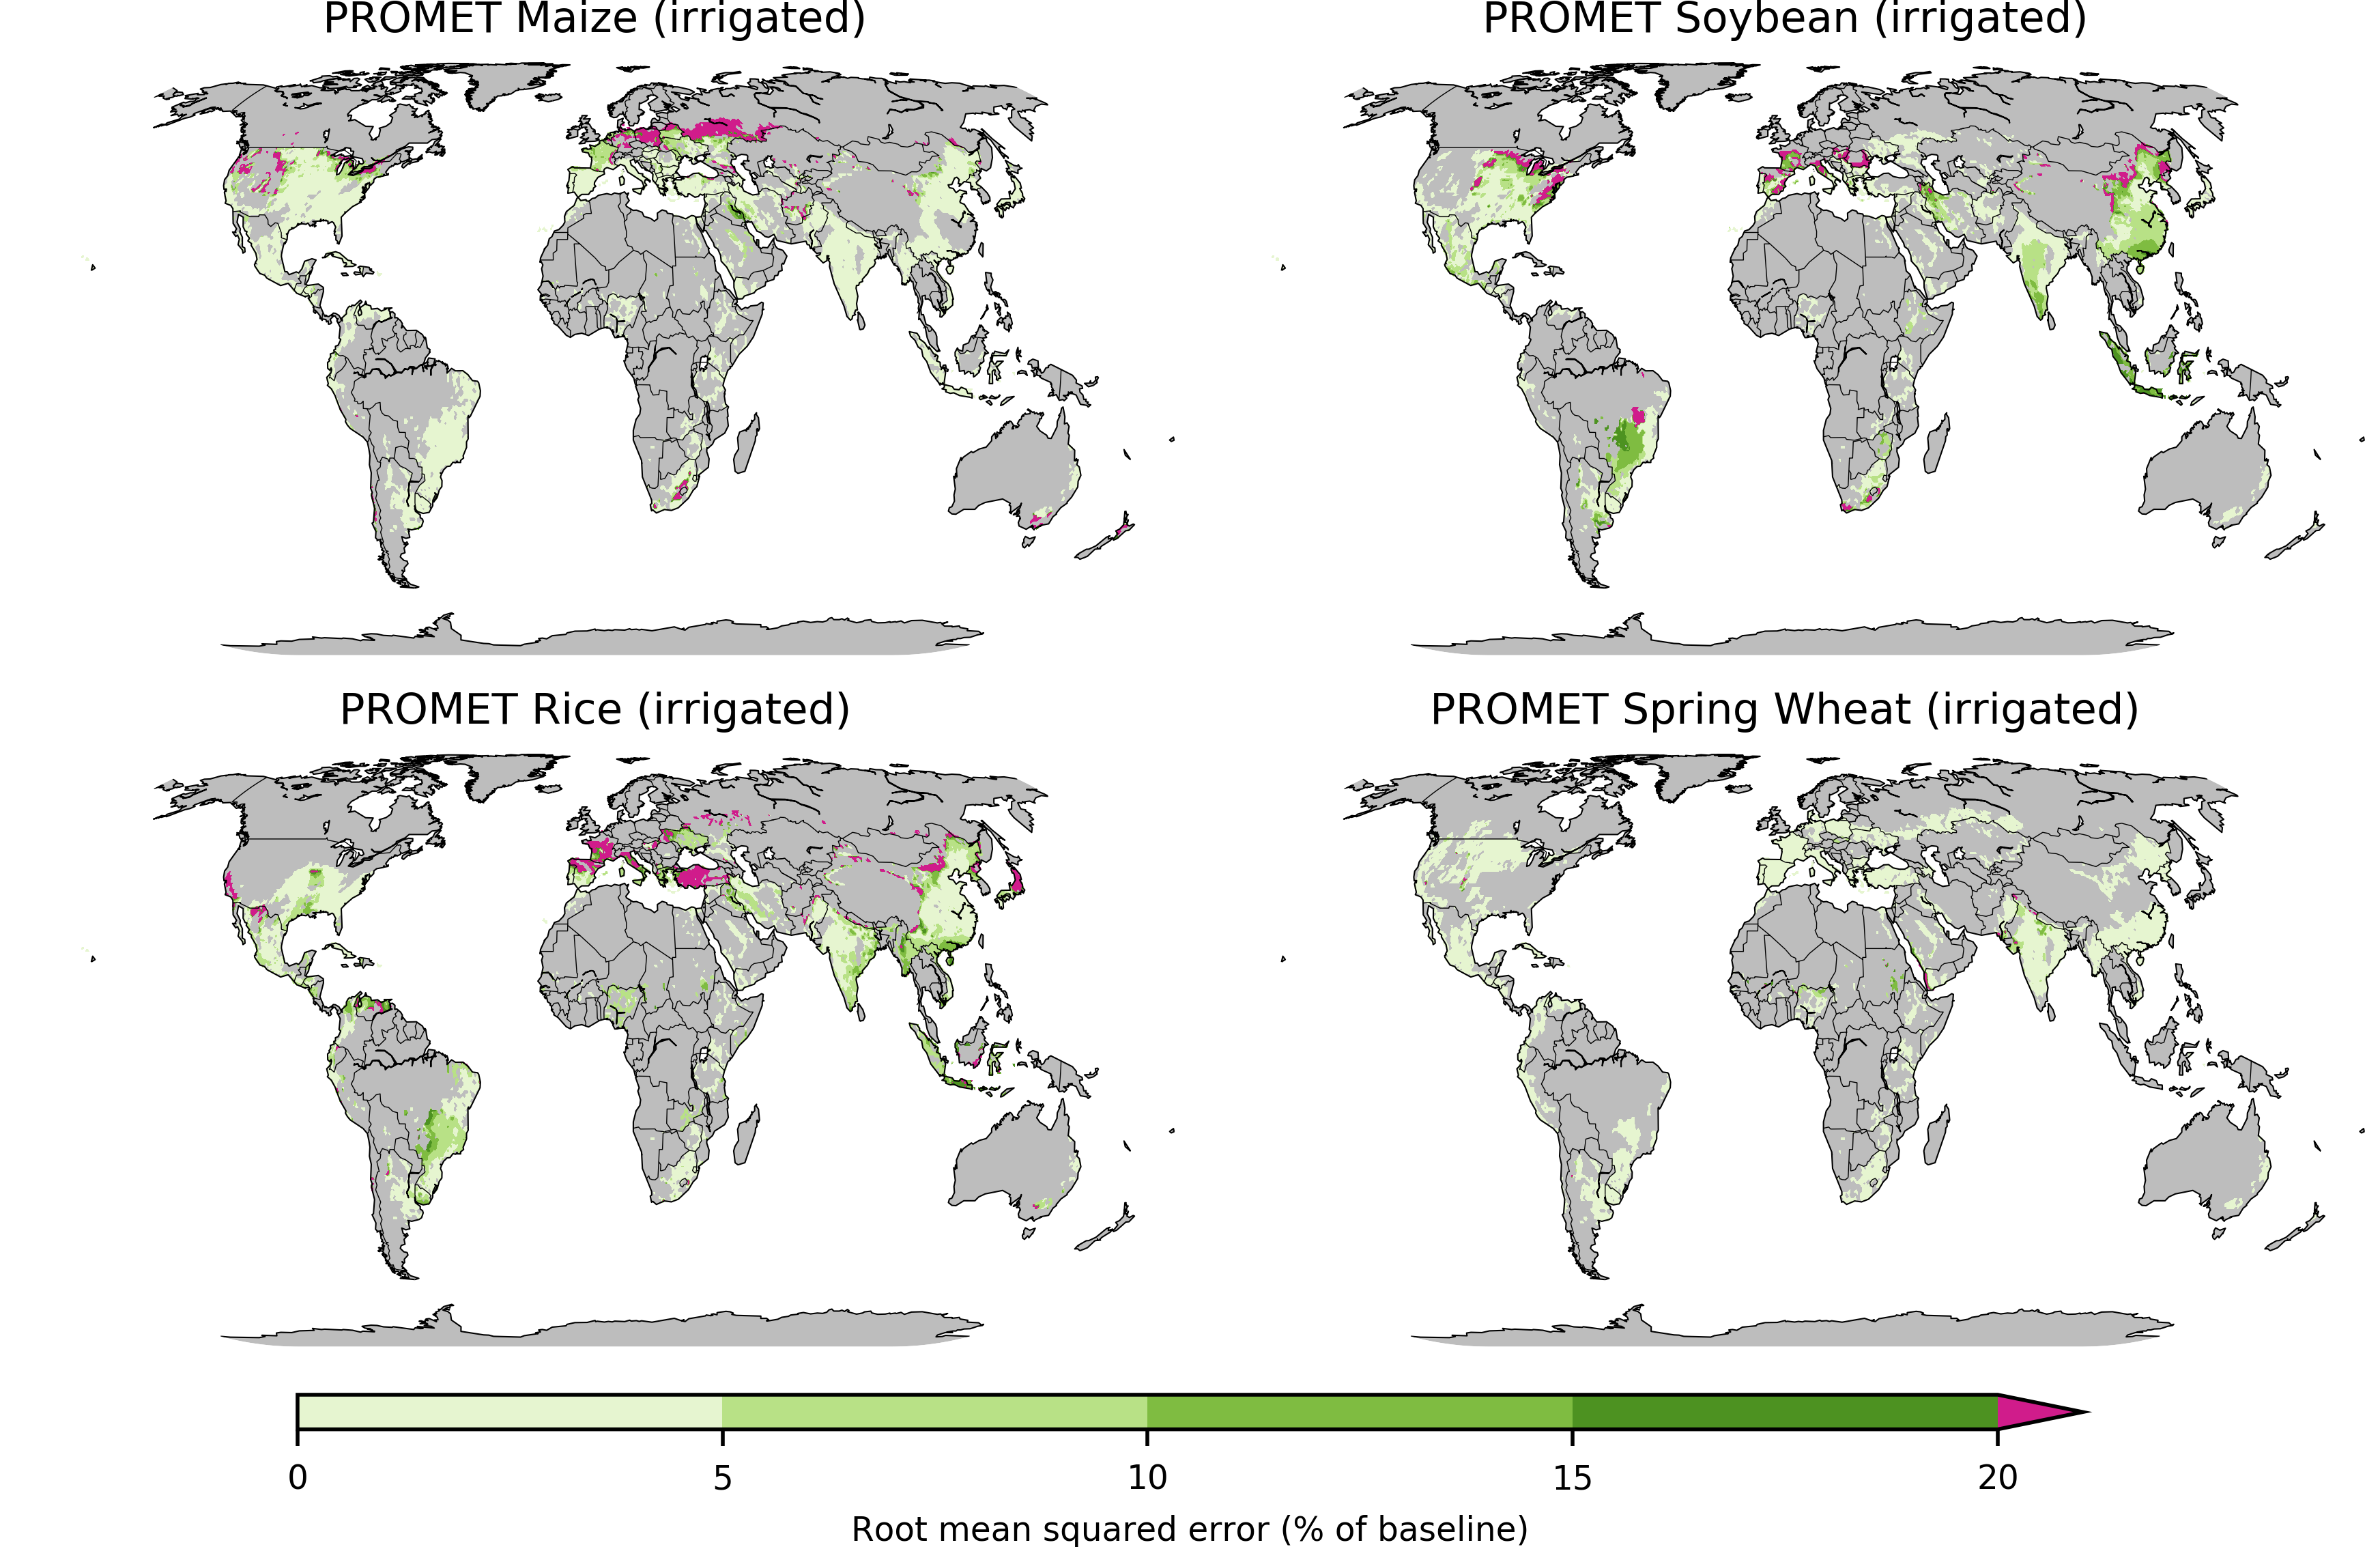
\includegraphics[width=15.5cm]{PROMET_spatial_MSE_ton_ha_irr.png}
\caption{Same as above for irrigated simulations.}
\label{fig:pdssatrmseirr}
\end{figure}

\begin{figure}[h!]
%S23
\centering
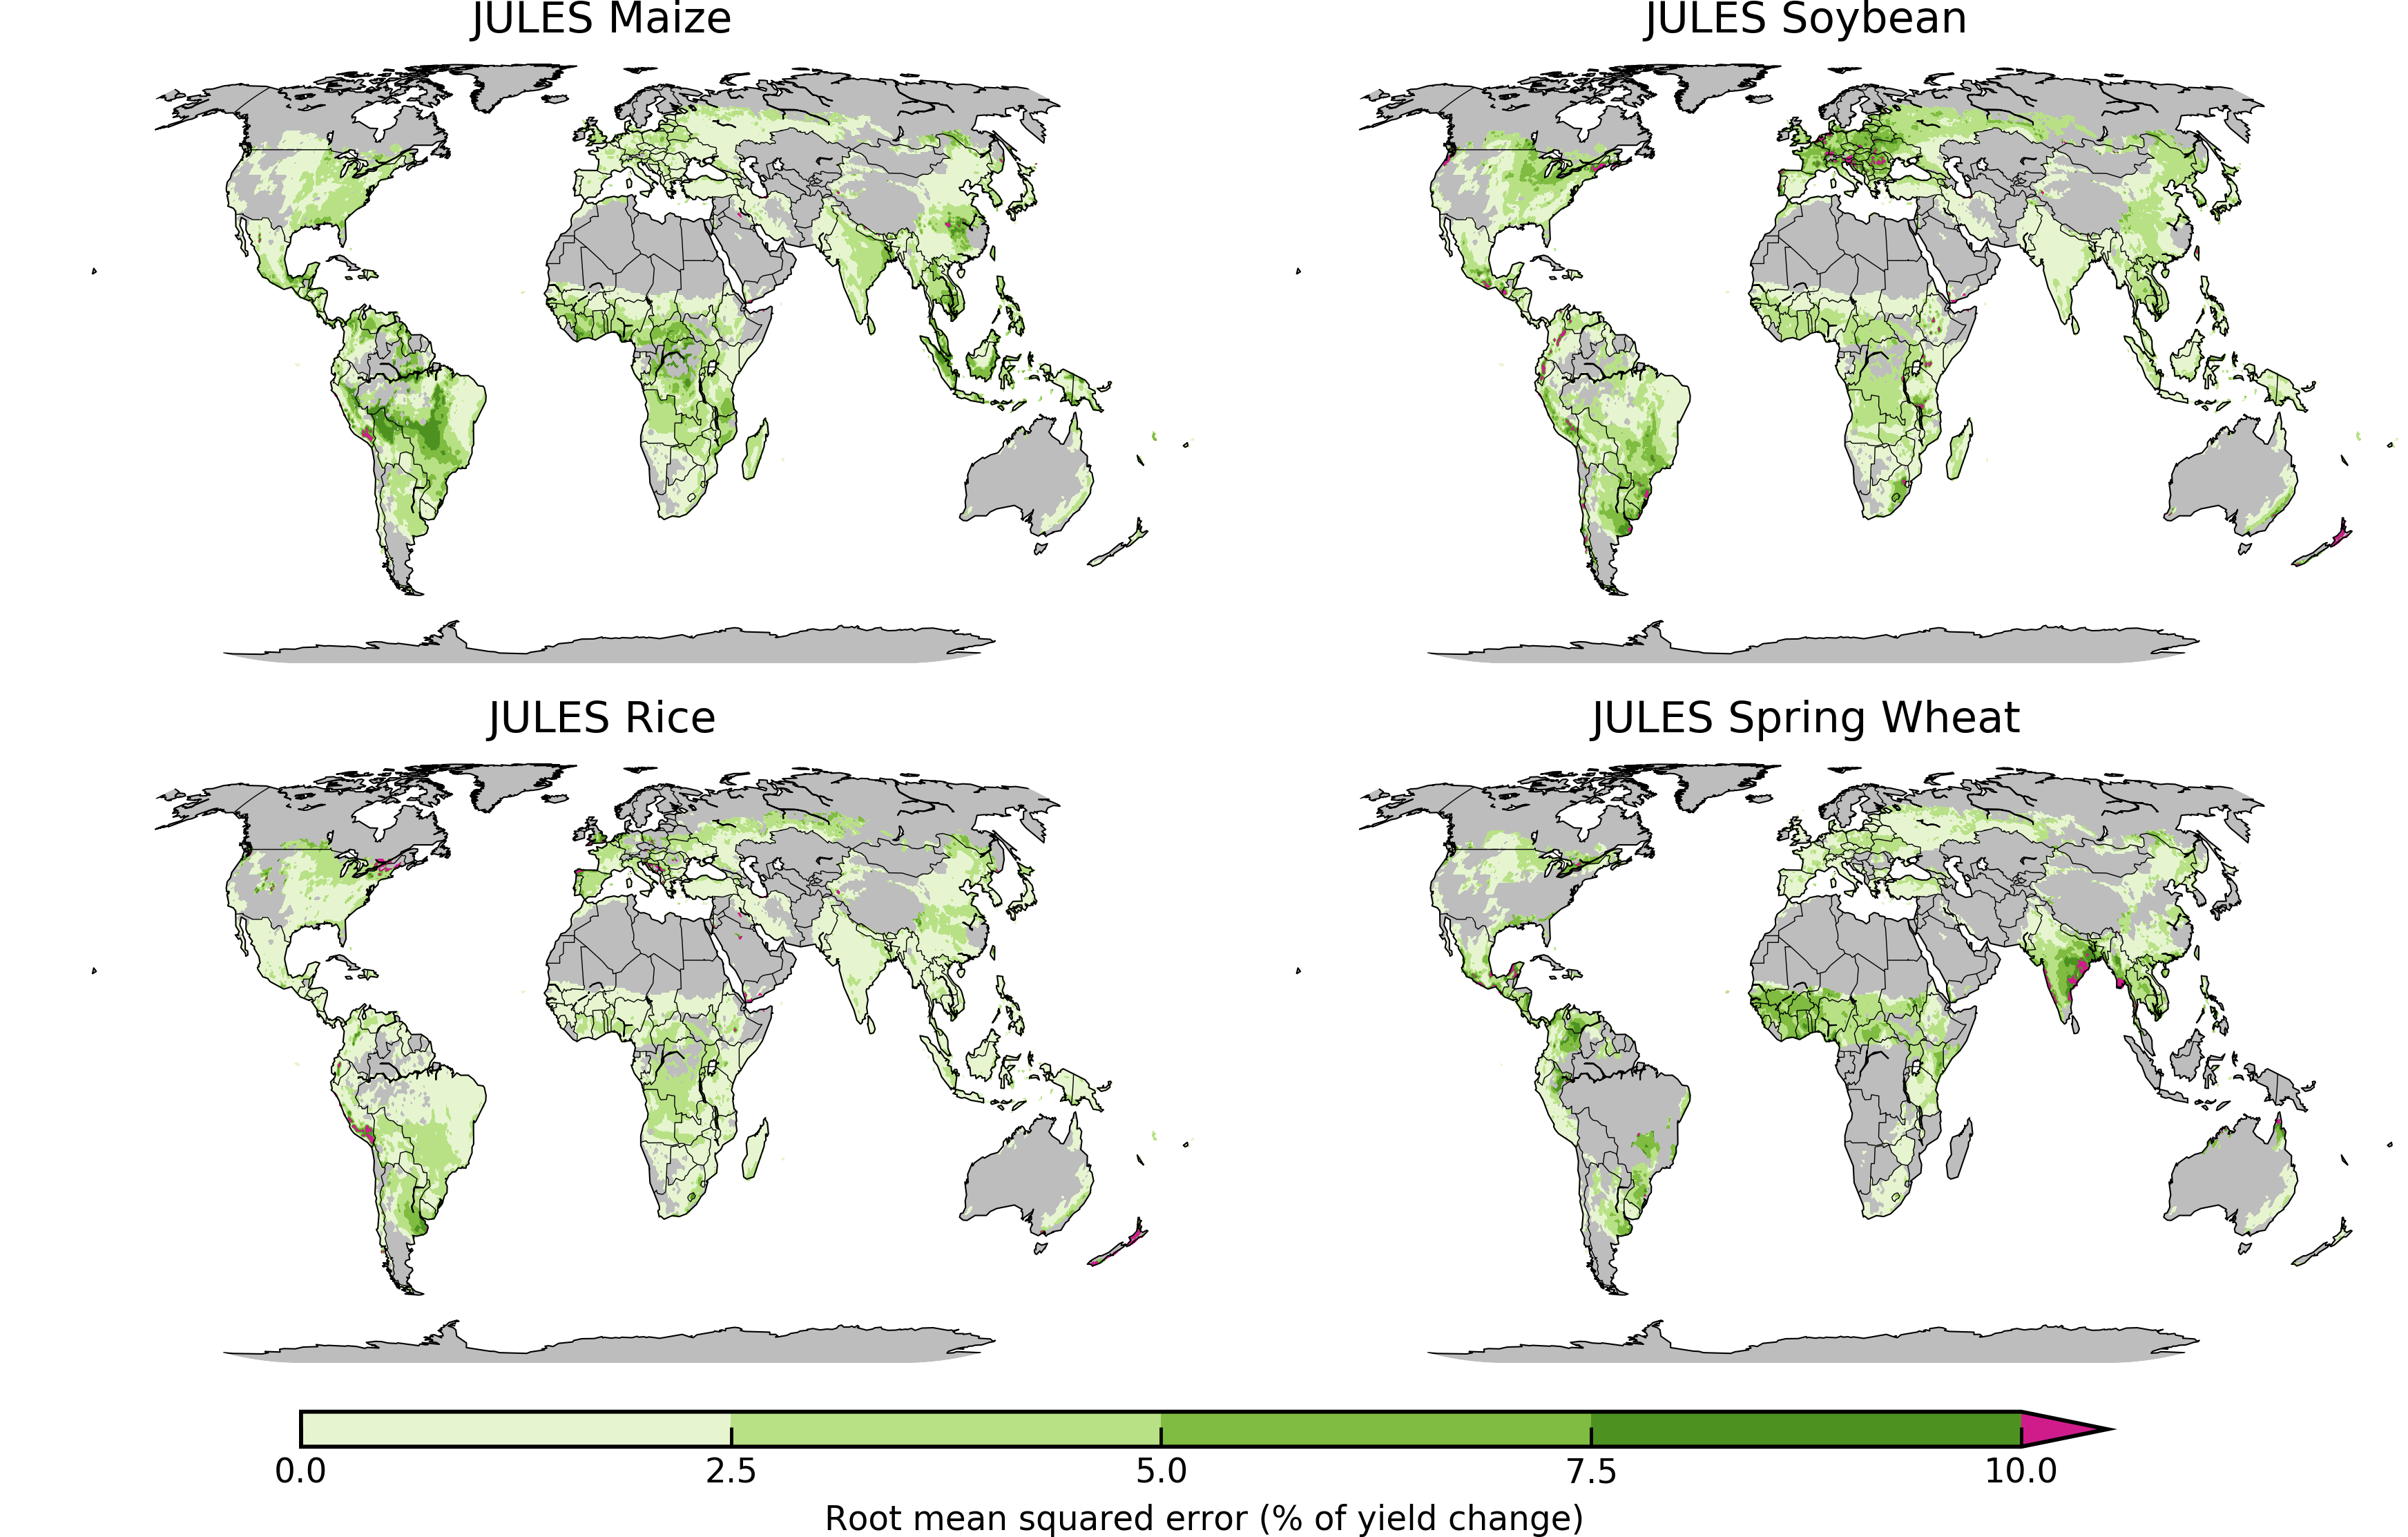
\includegraphics[width=15.5cm]{JULES_spatial_MSE_ton_ha.png}
\caption{Map of root mean squared error for three fold cross validation process for the JULES model for rainfed crops. Values shown as a percentage of baseline yield in each gridcell.}
\label{fig:pdssatrmse}
\end{figure}

\begin{figure}[h!]
%S24
\centering
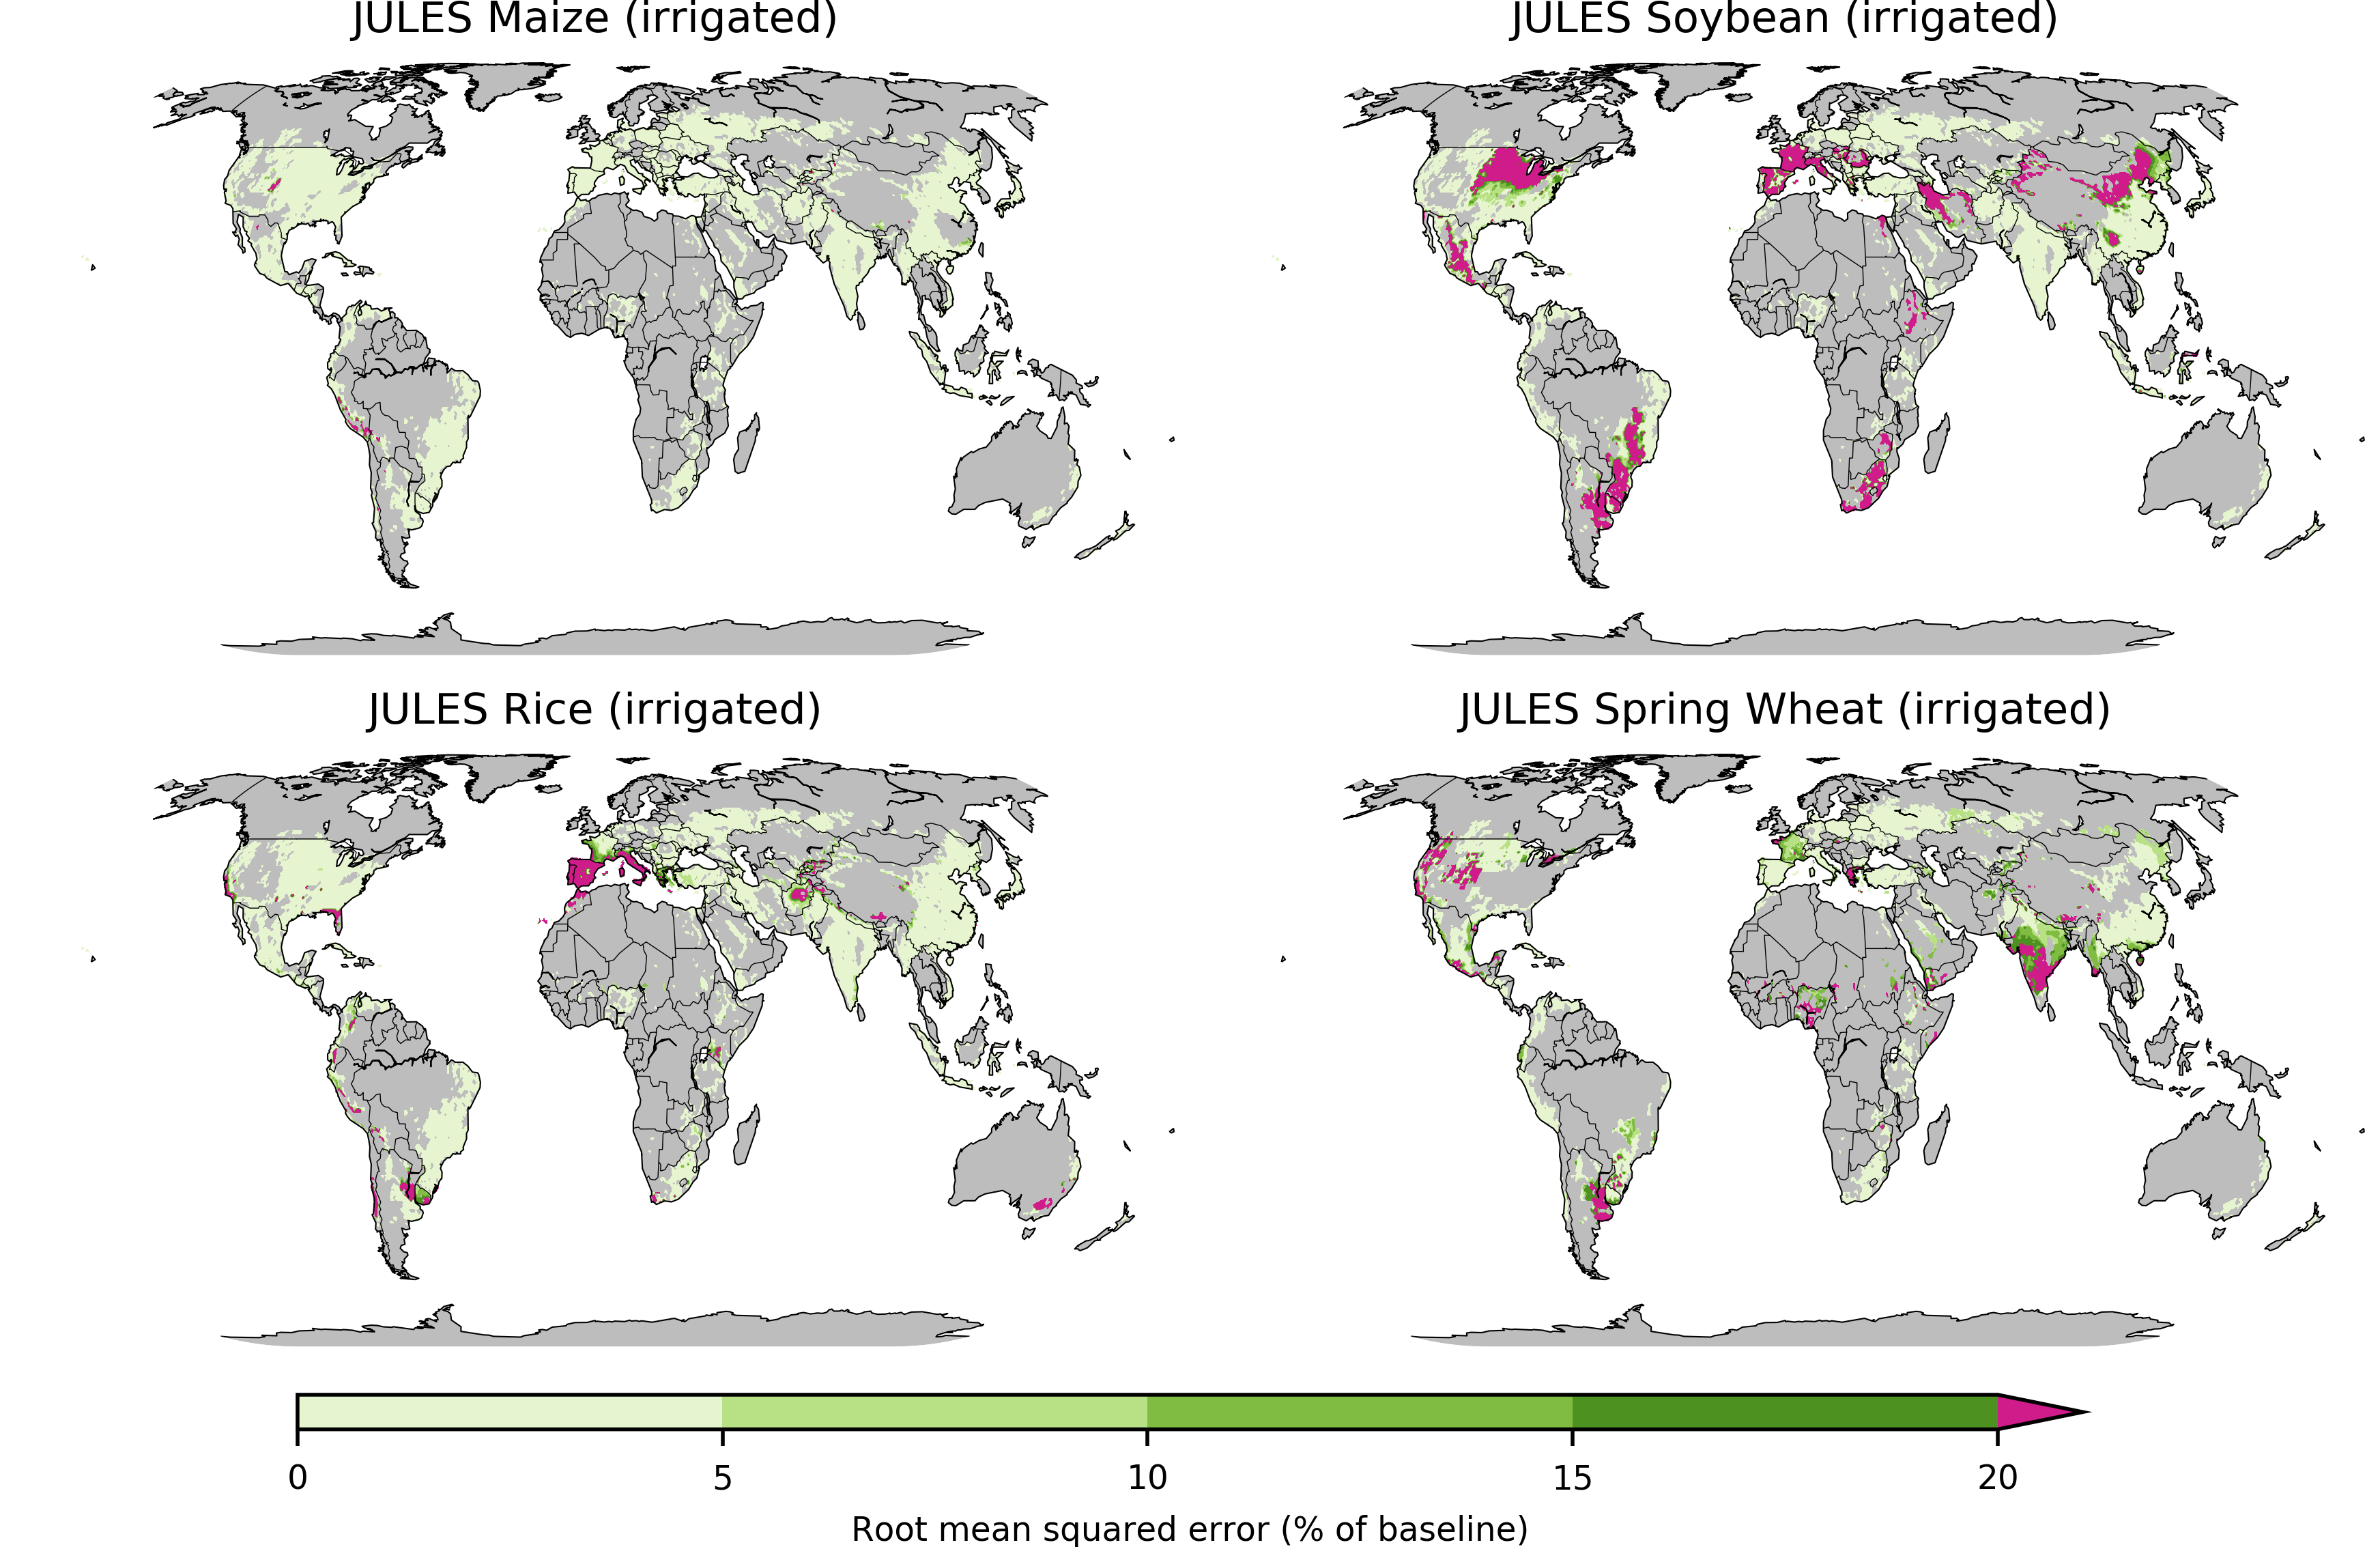
\includegraphics[width=15.5cm]{JULES_spatial_MSE_ton_ha_irr.png}
\caption{Same as above for irrigated simulations.}
\label{fig:pdssatrmseirr}
\end{figure}

\begin{figure}[h!]
%S25
\centering
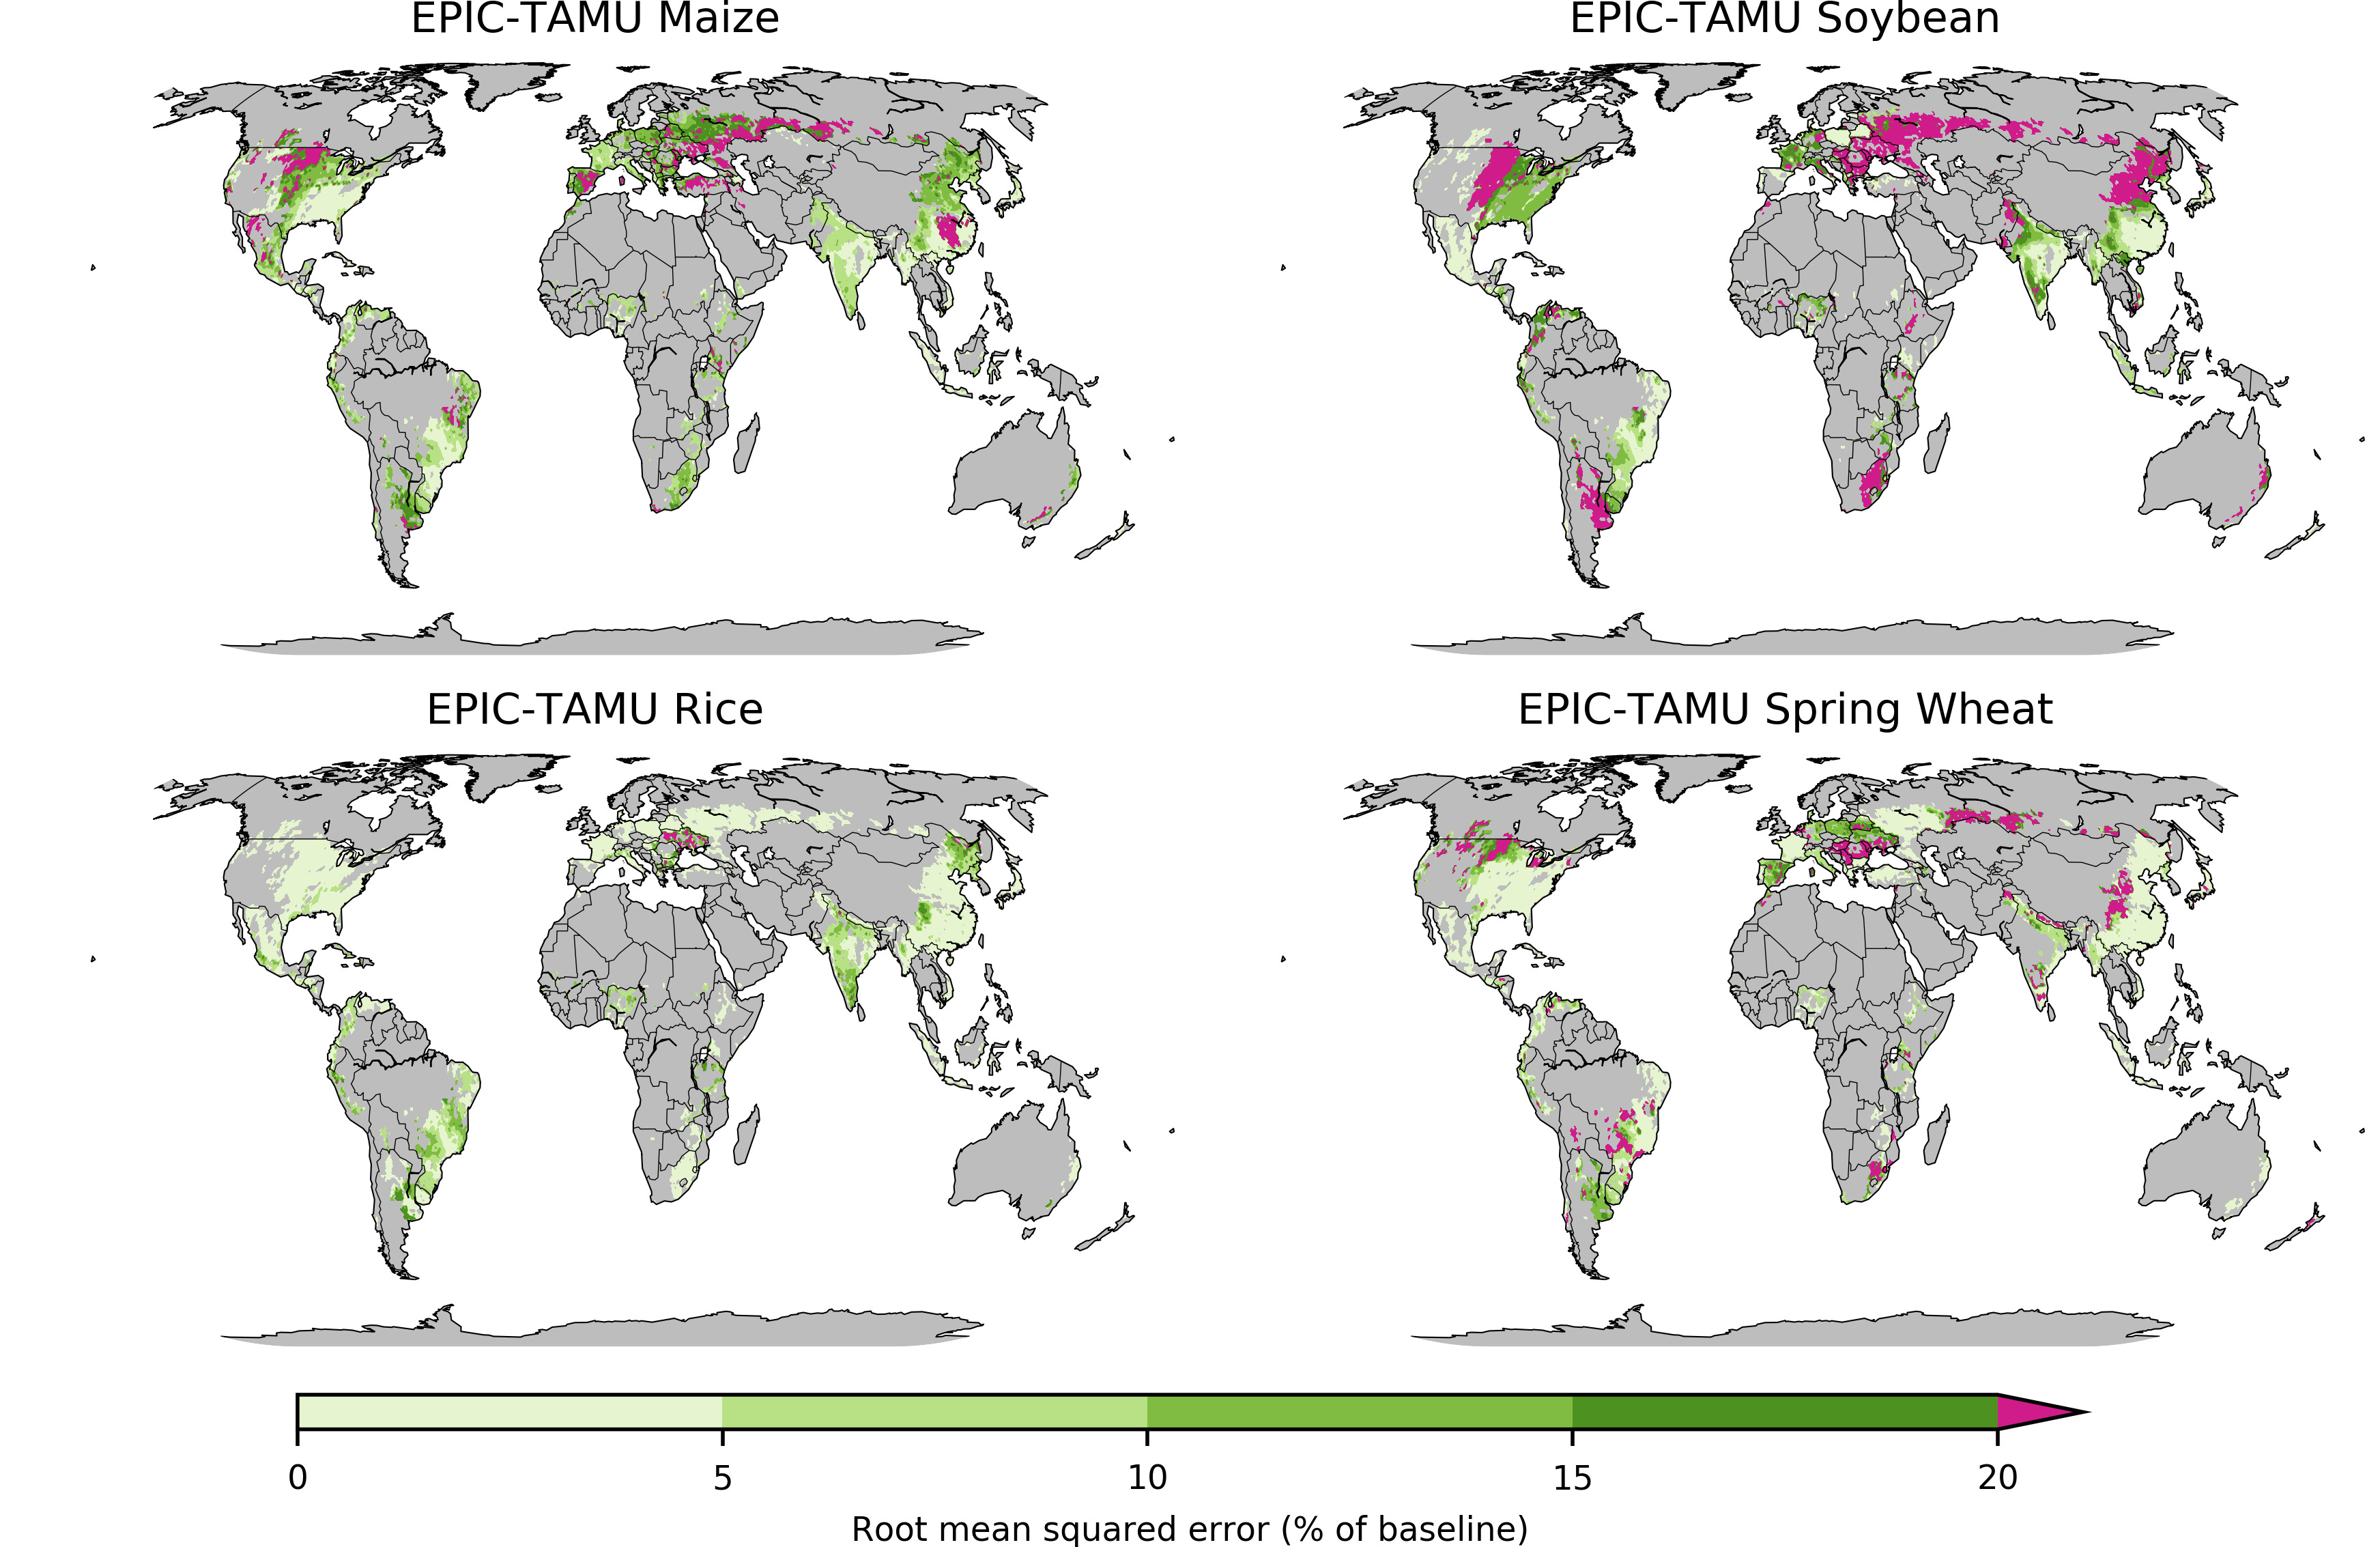
\includegraphics[width=15.5cm]{EPIC-TAMU_spatial_MSE_ton_ha.png}
\caption{Map of root mean squared error for three fold cross validation process for the EPIC-TAMU model for rainfed crops. Values shown as a percentage of baseline yield in each gridcell.}
\label{fig:pdssatrmse}
\end{figure}

\begin{figure}[h!]
%S26
\centering
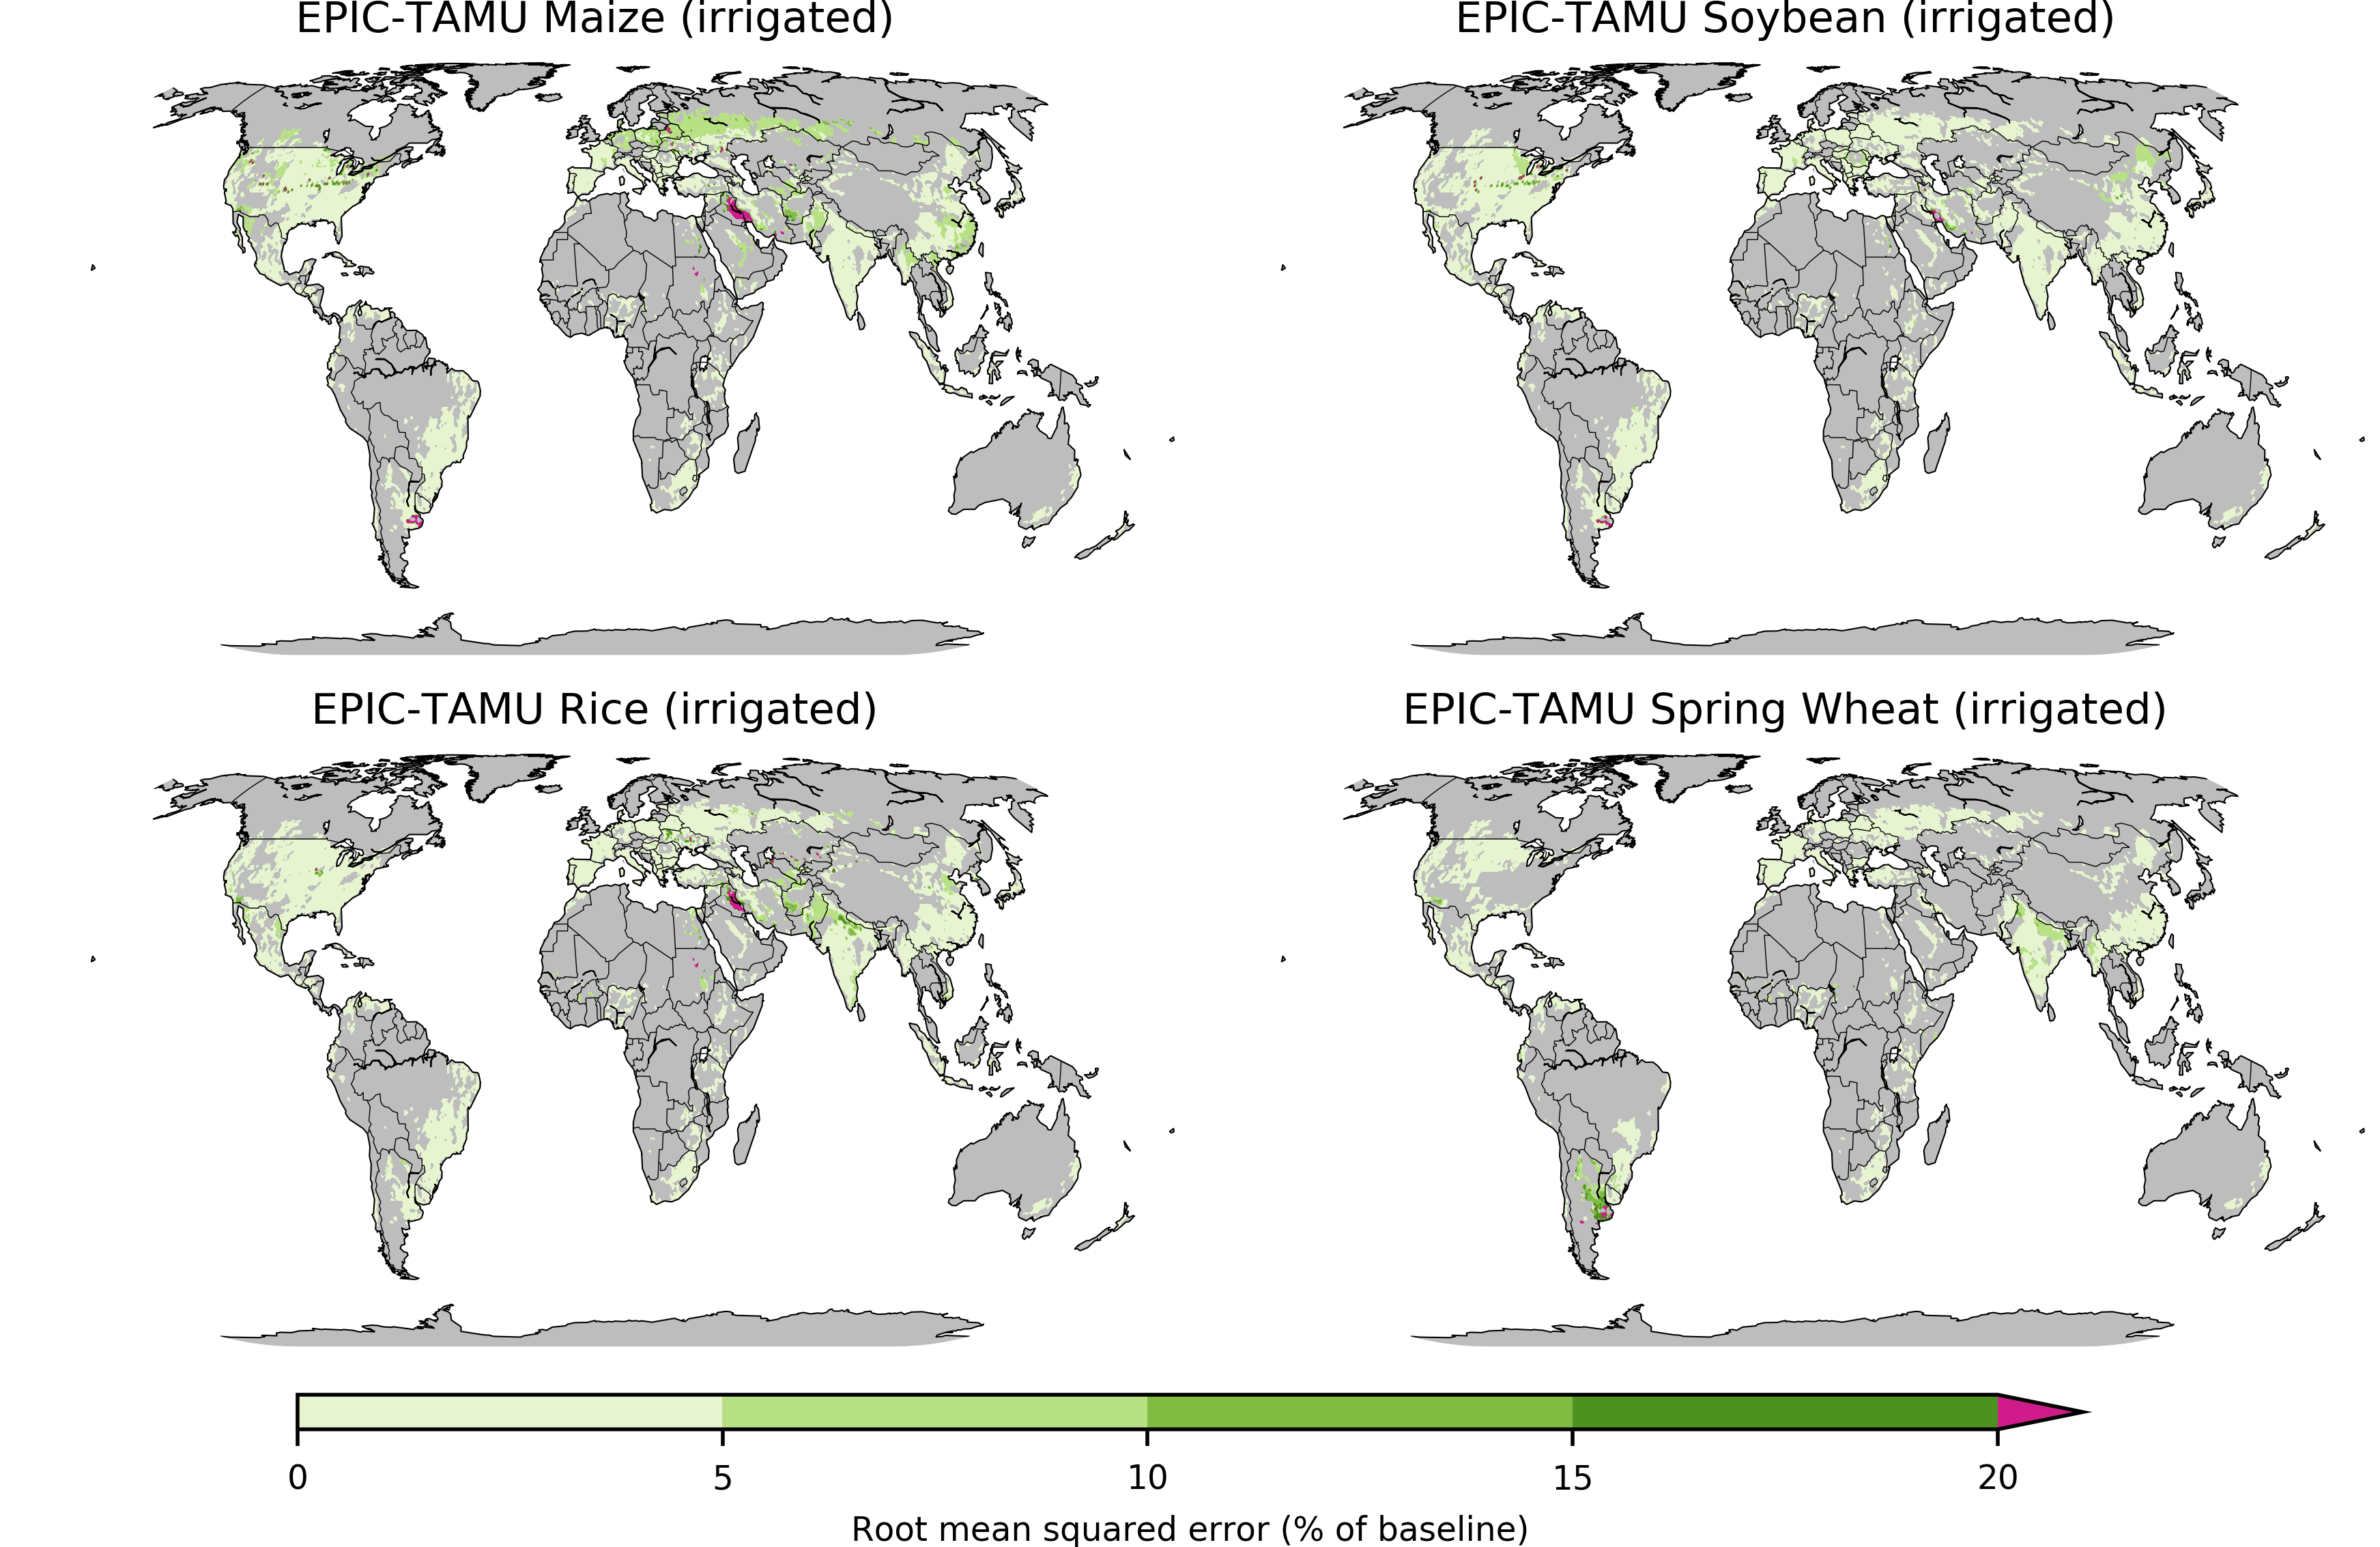
\includegraphics[width=15.5cm]{EPIC-TAMU_spatial_MSE_ton_ha_irr.png}
\caption{Same as above for irrigated simulations.}
\label{fig:pdssatrmseirr}
\end{figure}

\begin{figure}[h!]
%S27
\centering
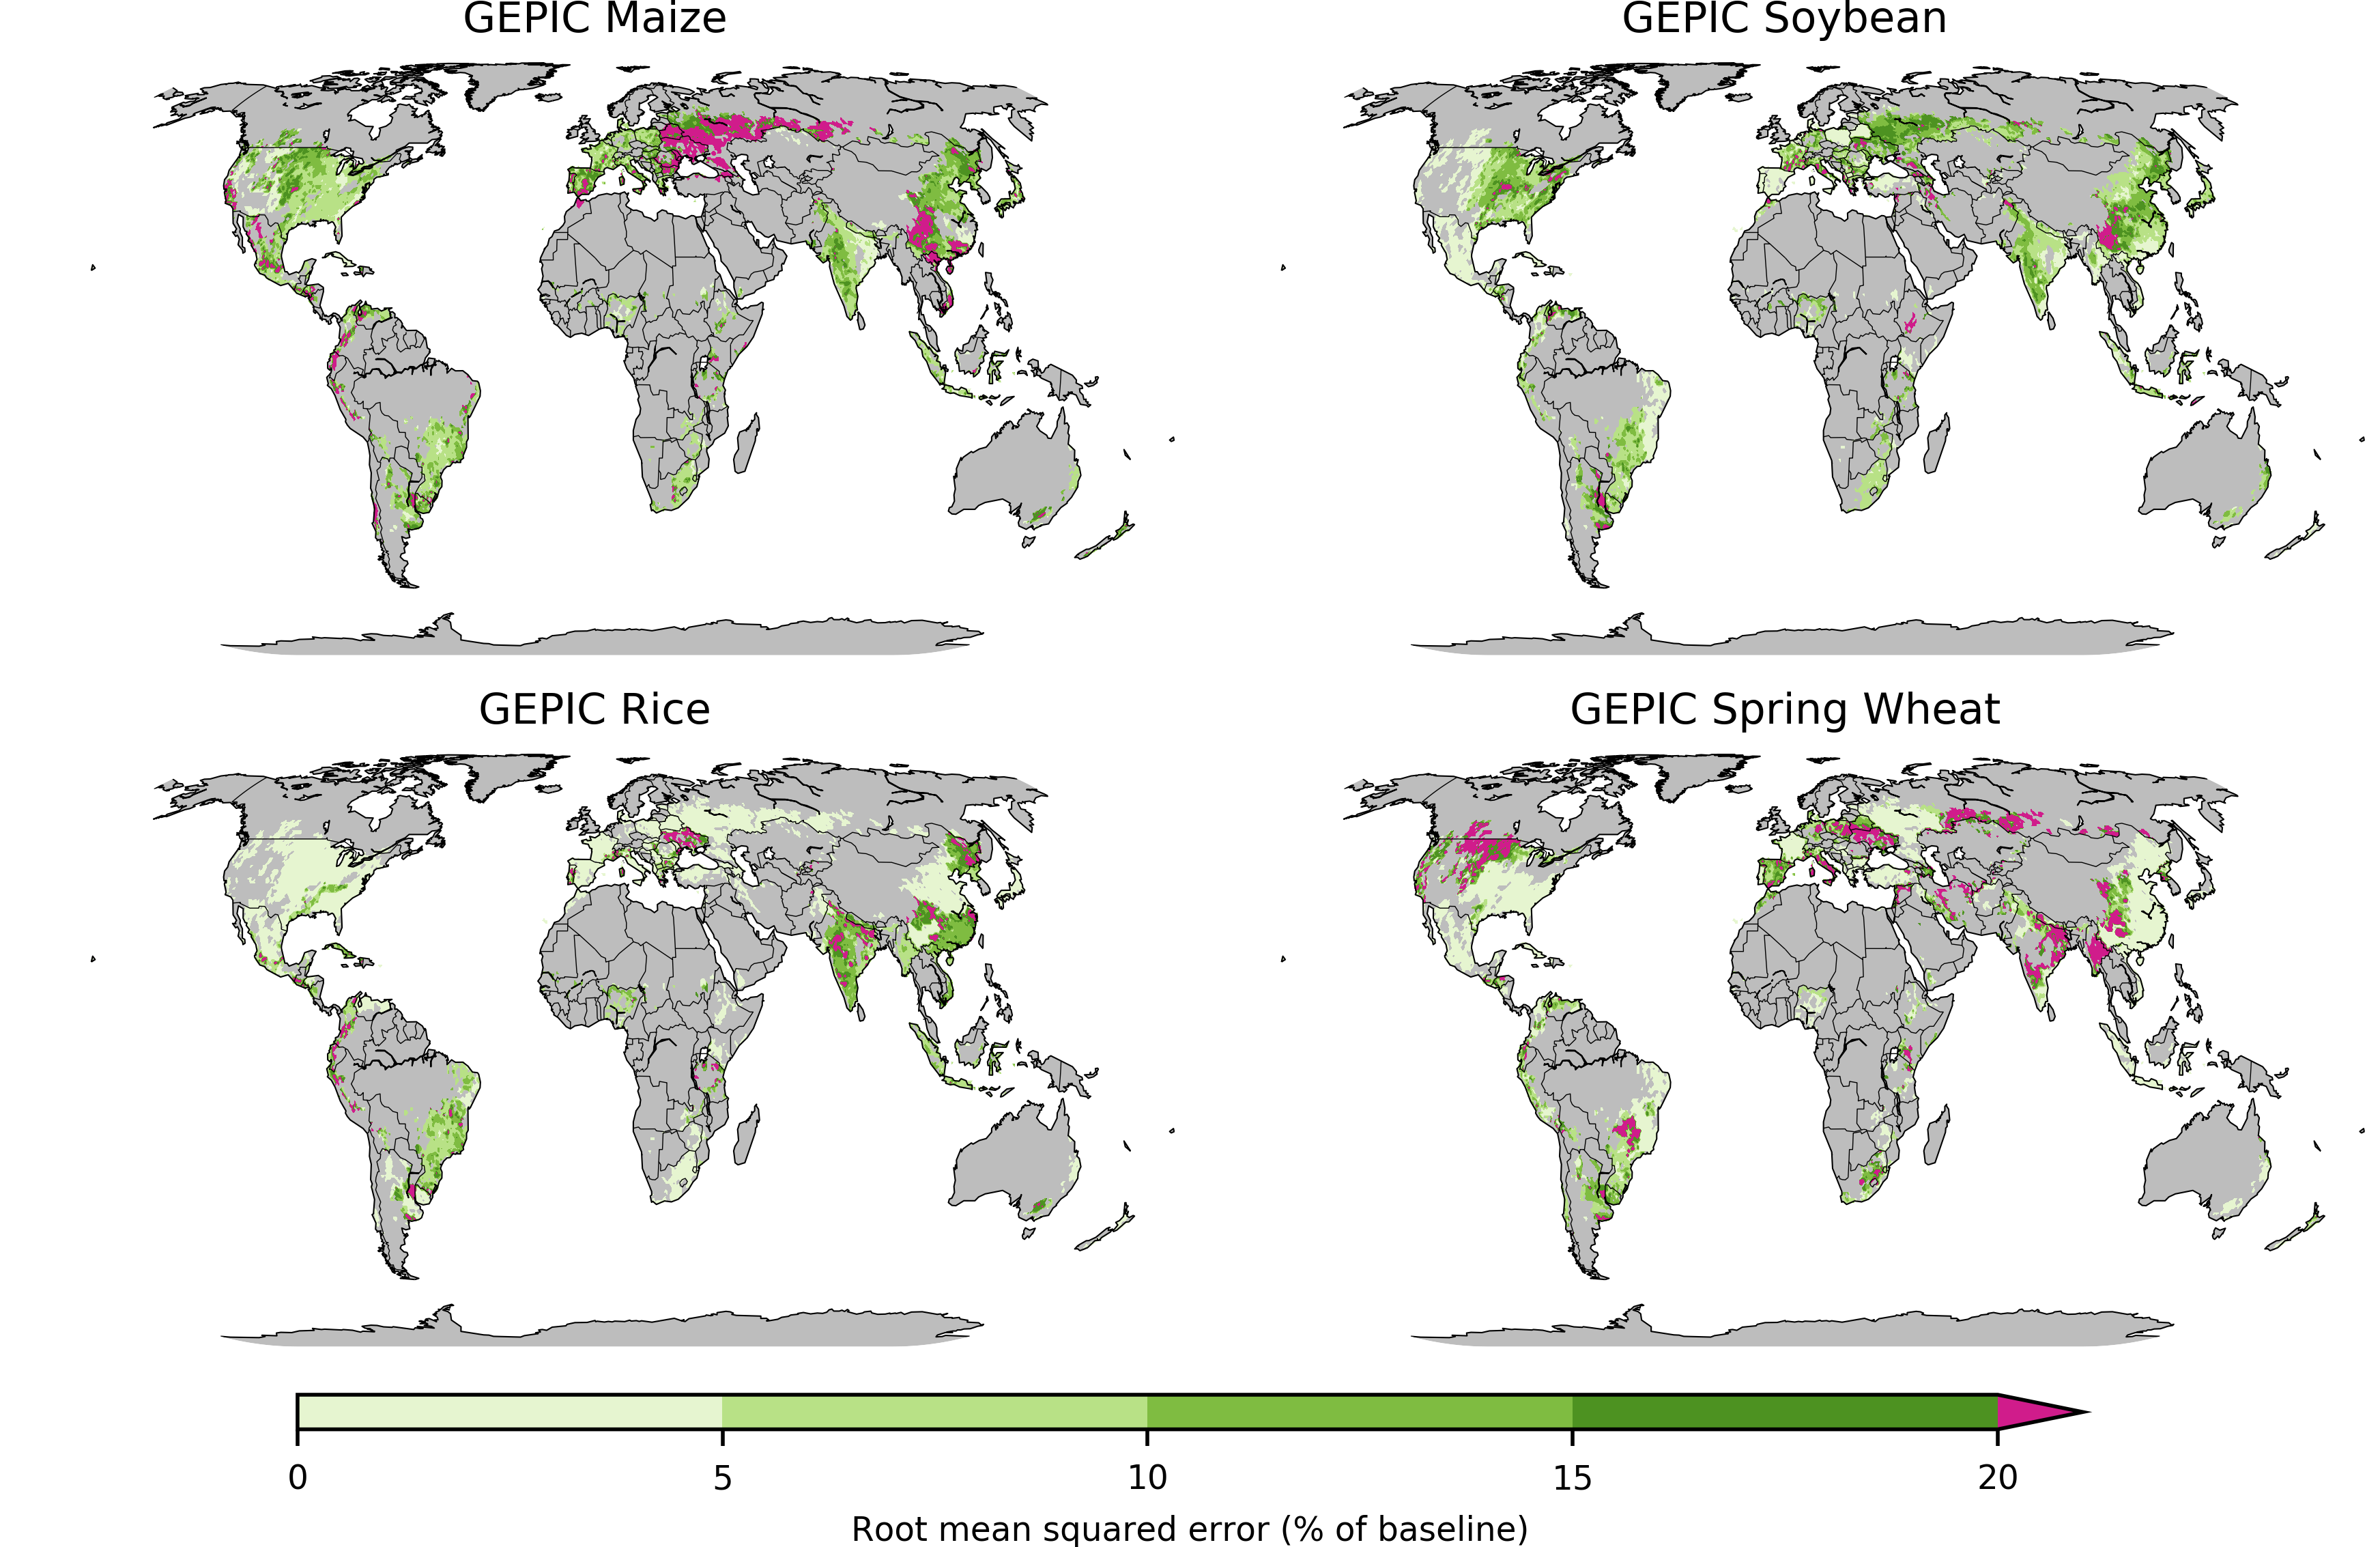
\includegraphics[width=15.5cm]{GEPIC_spatial_MSE_ton_ha.png}
\caption{Map of root mean squared error for three fold cross validation process for the GEPIC model for rainfed crops. Values shown as a percentage of baseline yield in each gridcell.}
\label{fig:pdssatrmse}
\end{figure}

\begin{figure}[h!]
%S28
\centering
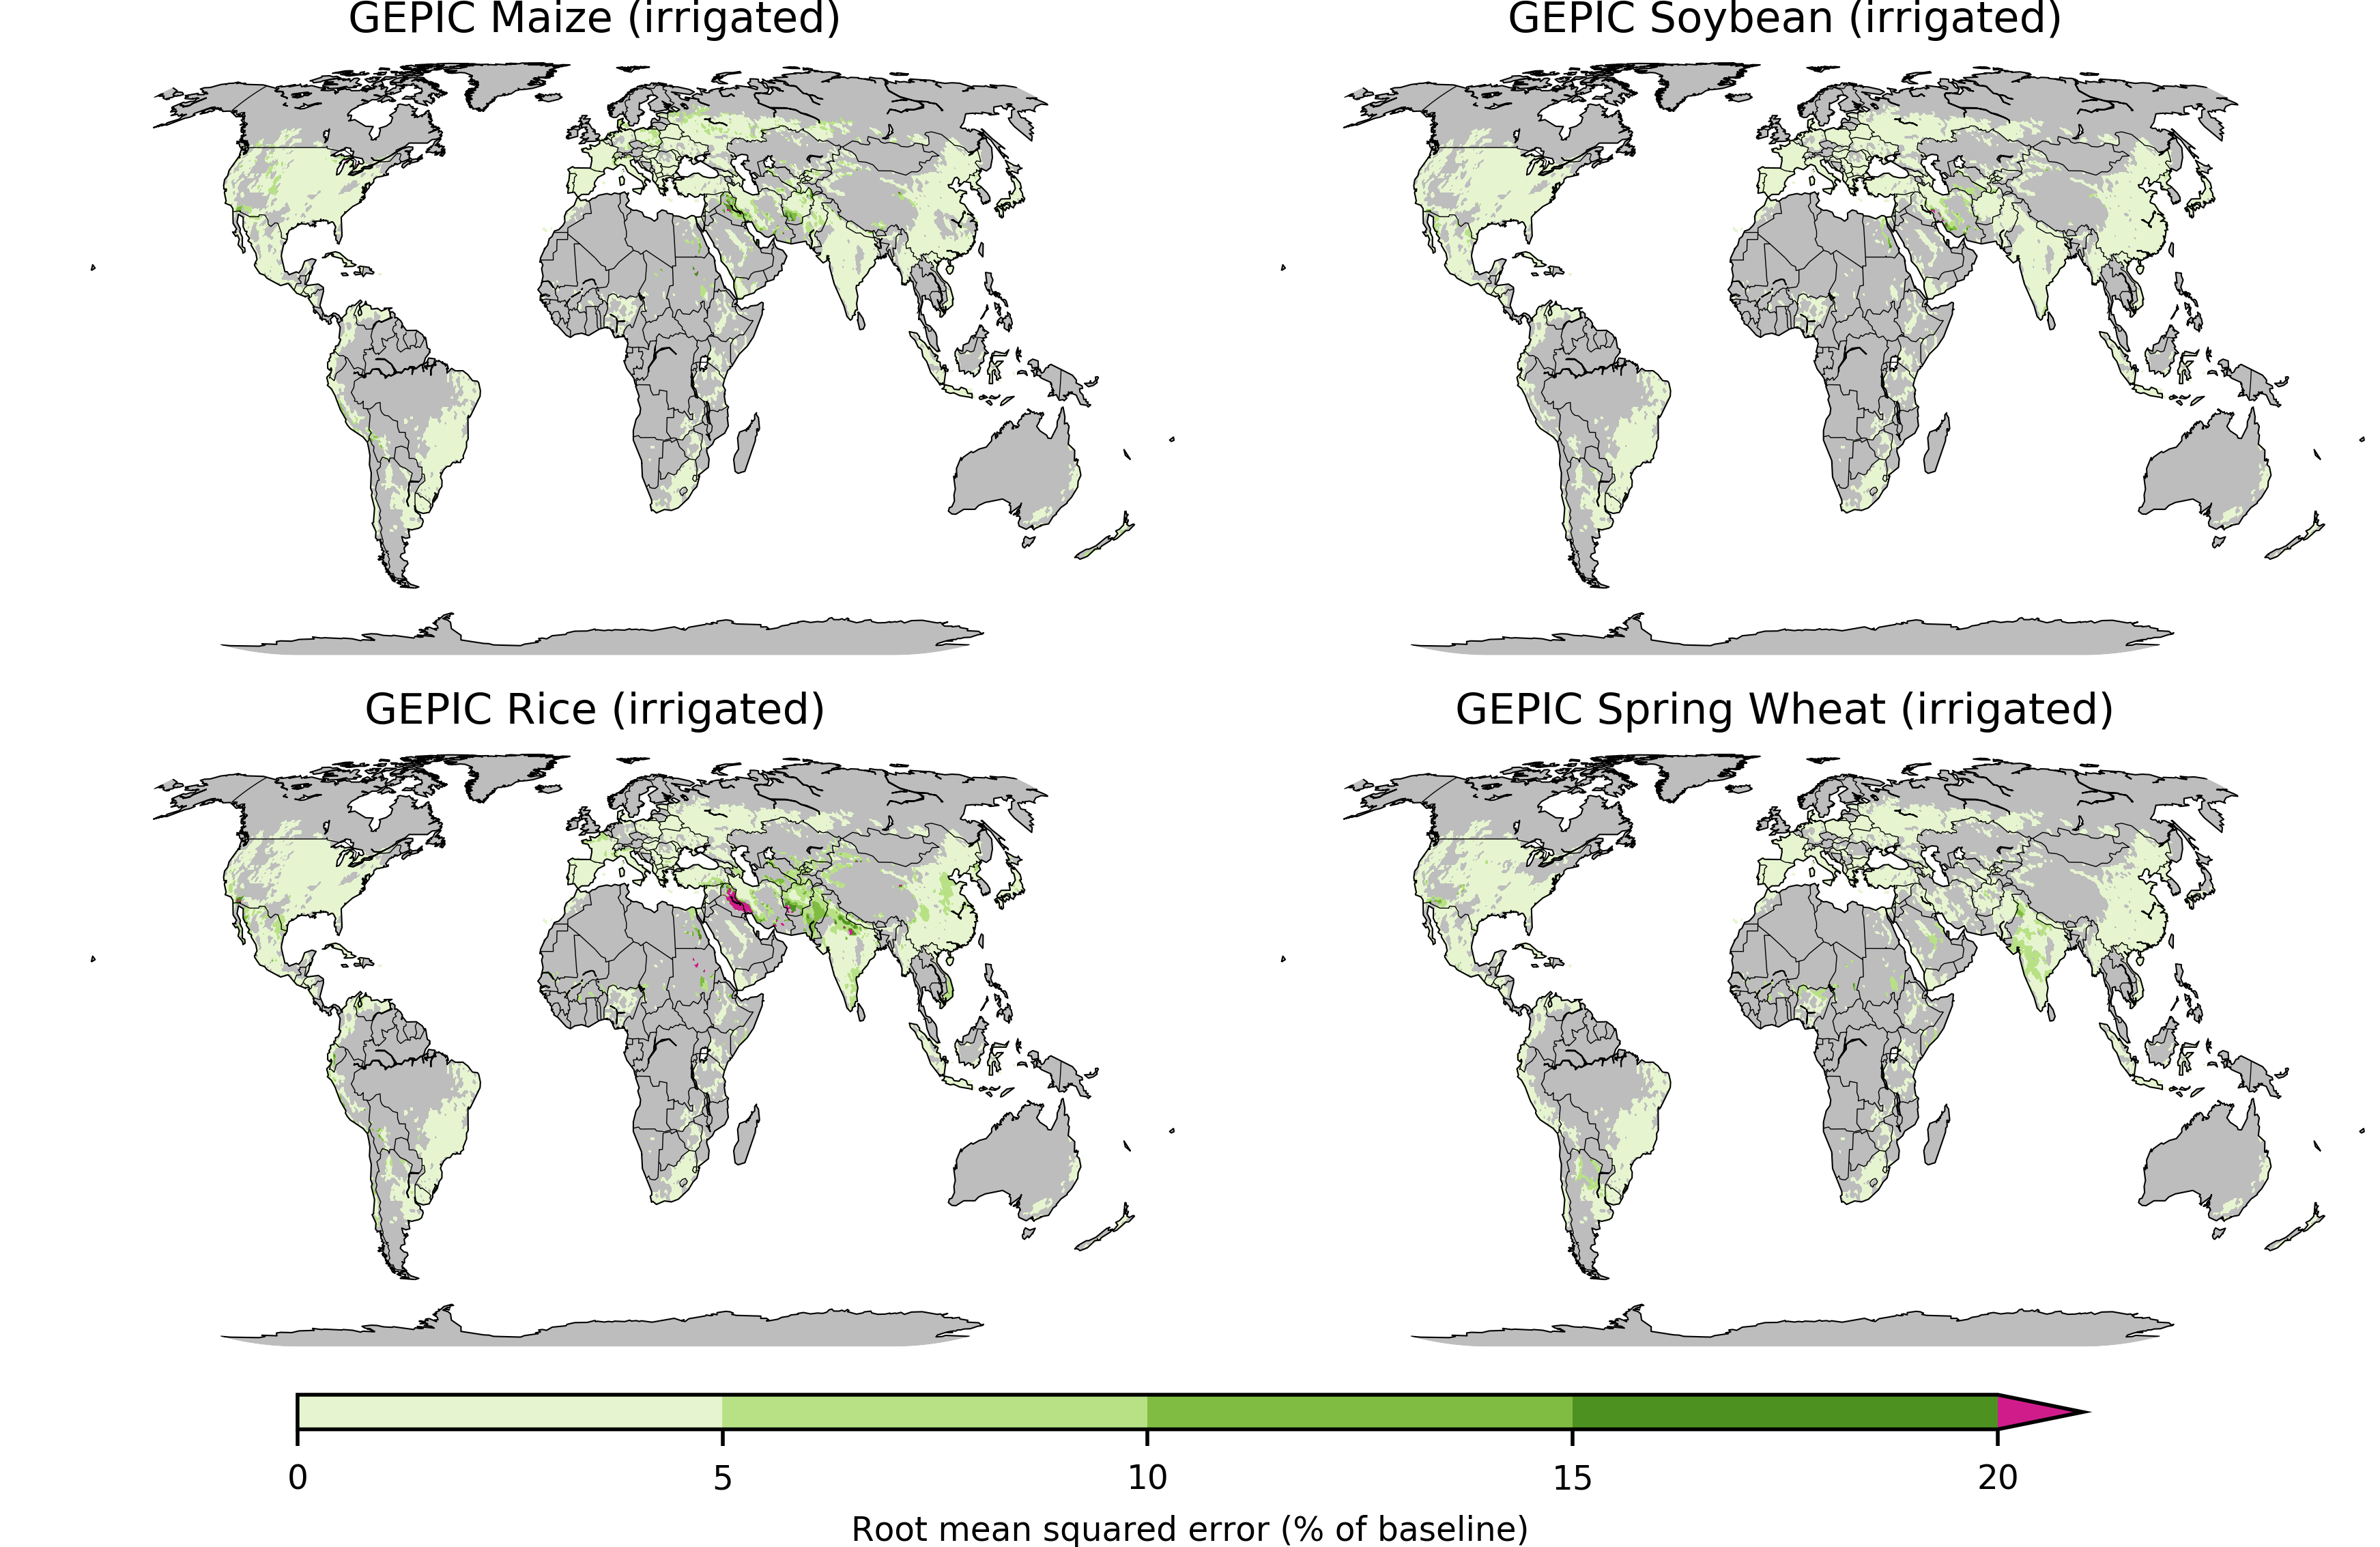
\includegraphics[width=15.5cm]{GEPIC_spatial_MSE_ton_ha_irr.png}
\caption{Same as above for irrigated simulations.}
\label{fig:pdssatrmseirr}
\end{figure}

\begin{figure}[h!]
%S29
\centering
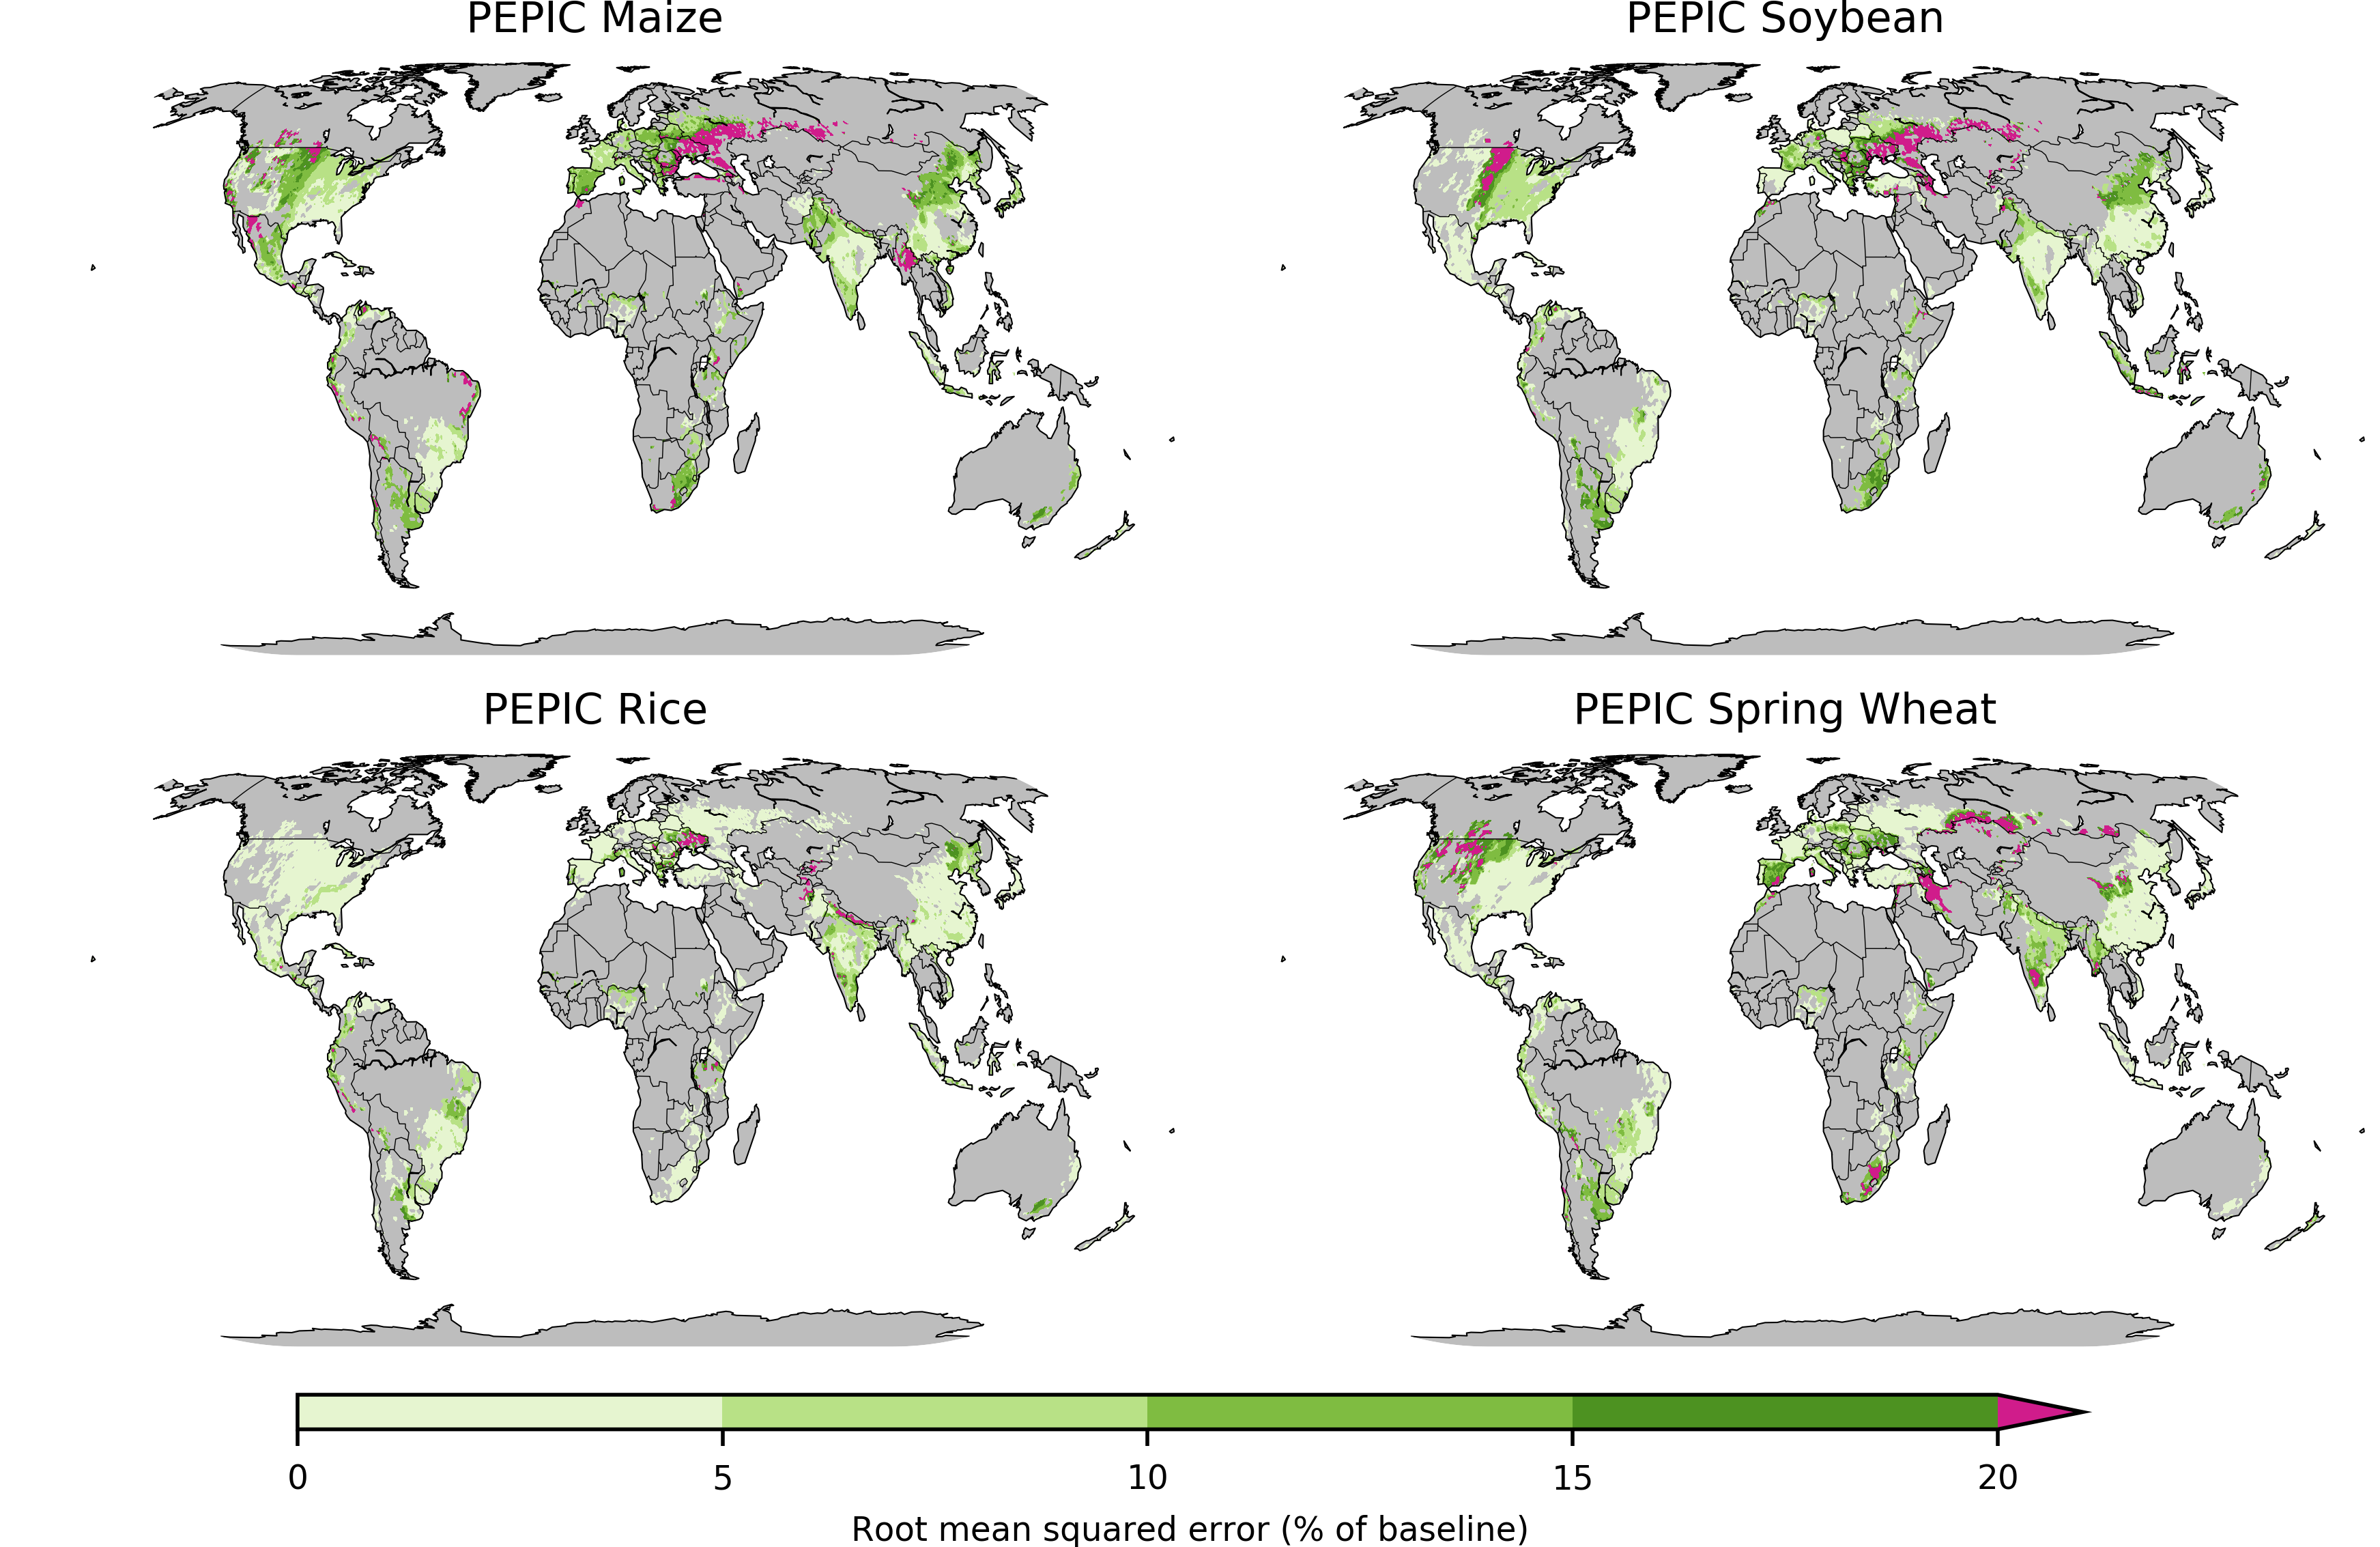
\includegraphics[width=15.5cm]{PEPIC_spatial_MSE_ton_ha.png}
\caption{Map of root mean squared error for three fold cross validation process for the PEPIC model for rainfed crops. Values shown as a percentage of baseline yield in each gridcell.}
\label{fig:pdssatrmse}
\end{figure}

\begin{figure}[h!]
%S30
\centering
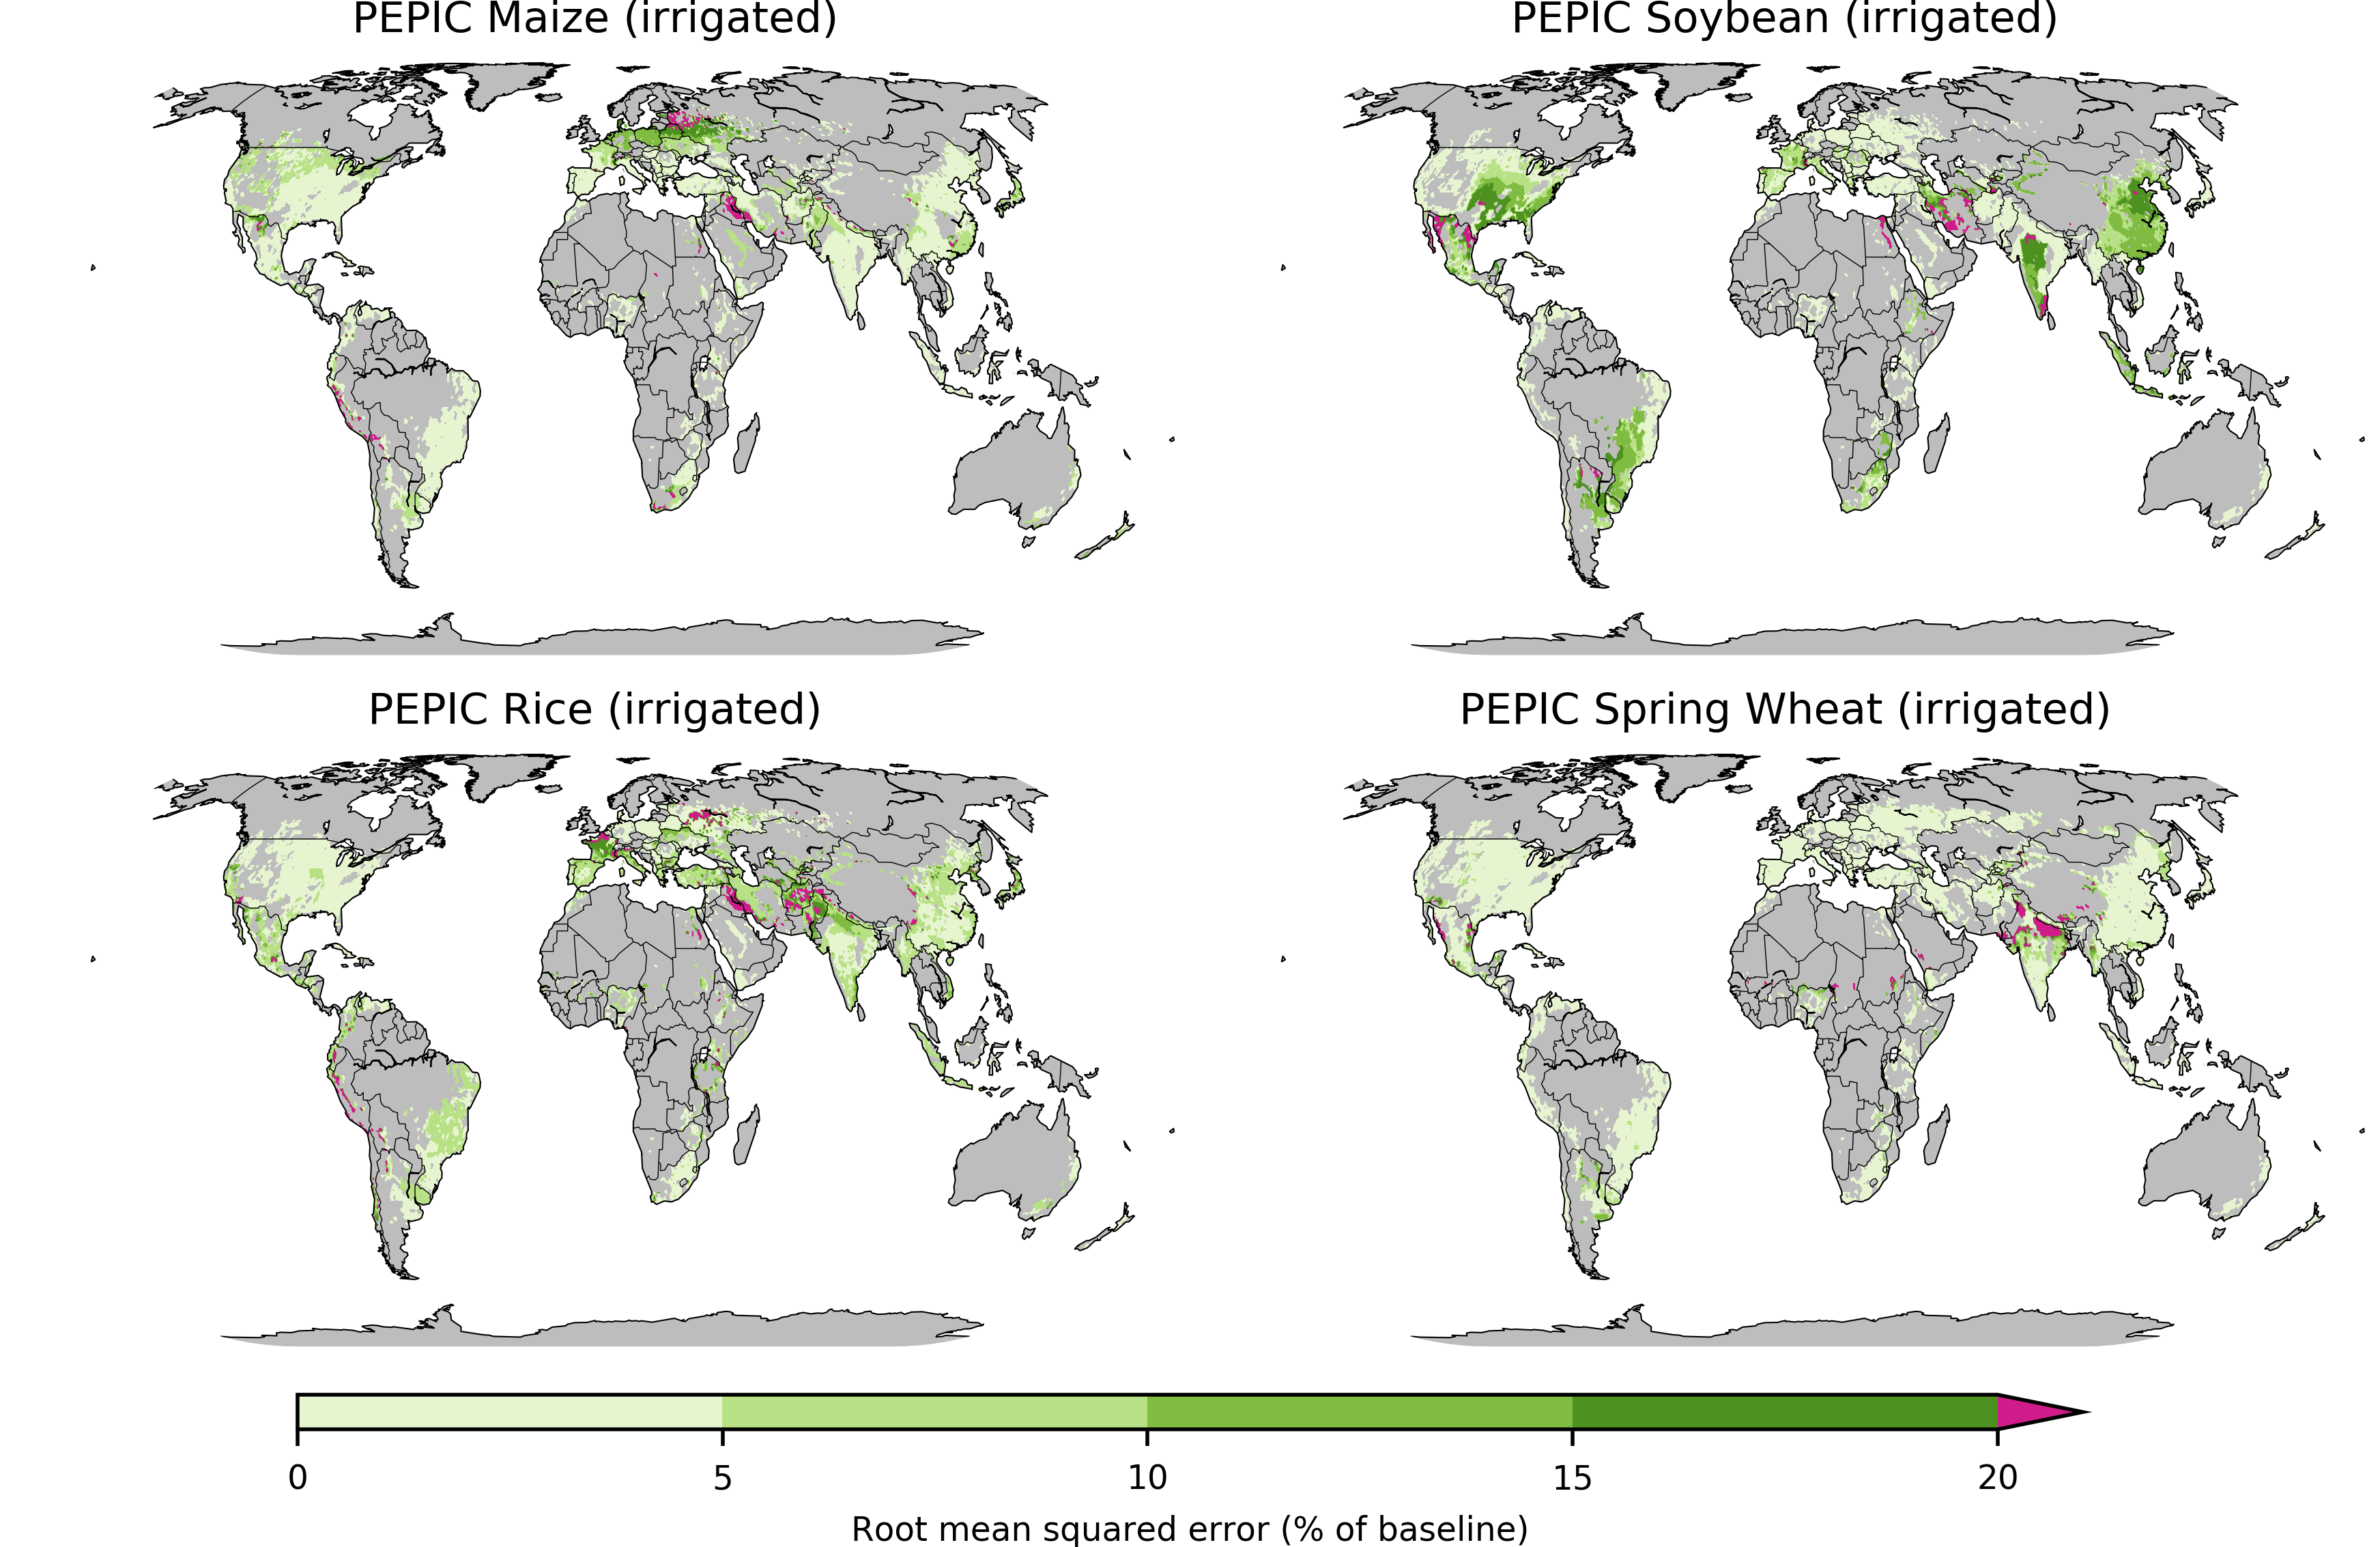
\includegraphics[width=15.5cm]{PEPIC_spatial_MSE_ton_ha_irr.png}
\caption{Same as above for irrigated simulations.}
\label{fig:pdssatrmseirr}
\end{figure}

\end{document}


%%%%%%%%%%%%%%%%%%%%%%%%%%%%%%%%%%%%%%%%%%%%%%%%%%%%%%%%%%%%%%%%%%%%%%%%%%%%%%%%%%%%%%%%%%%%%%%%%%%%%%%%%%%%%%%%
%%%%%%%%%%%%%%%%%%%%%%%%%%%%%%%%%%%%%%%%%%%%%%%%%%%%%%%%%%%%%%%%%%%%%%%%%%%%%%%%%%%%%%%%%%%%%%%%%%%%%%%%%%%%%%%%
%%%%%%%%%%%%%%%%%%%%%%%%%%%%%%%%%%%%%%%%%%%%%%%%%%%%%%%%%%%%%%%%%%%%%%%%%%%%%%%%%%%%%%%%%%%%%%%%%%%%%%%%%%%%%%%%
%%%%%%%%%%%%%%%%%%%%%%%%%%%%%%%%%%%%%%%%%%%%%%%%%%%%%%%%%%%%%%%%%%%%%%%%%%%%%%%%%%%%%%%%%%%%%%%%%%%%%%%%%%%%%%%%


\centering{James Franke$^{1, 2}$, 
Joshua Elliott$^{2, 3}$, 
Christoph M\"{u}ller$^4$, 
Alexander Ruane$^5$, 
Abigail Snyder$^6$,\\ 
Jonas J\"{a}germeyr$^{3, 2, 4, 5}$, 
Juraj Balkovic$^{7, 8}$, 
Philippe Ciais$^{9, 10}$, 
Marie Dury$^{11}$, 
Pete Falloon$^{12}$,\\ 
Christian Folberth$^7$, 
Louis Fran{\c{c}}ois$^{11}$, 
Tobias Hank$^{13}$, 
Munir Hoffmann$^{14,23}$, 
Cesar Izaurralde$^{15, 16}$,\\ 
Ingrid Jacquemin$^11$, 
Curtis Jones$^{15}$, 
Nikolay Khabarov$^7$, 
Marian Koch$^{14}$, 
Michelle Li$^{2, 17}$, 
Wenfeng Liu$^{18, 9}$,\\ 
Stefan Olin$^{19}$, 
Meridel Phillips$^{5, 20}$, 
Thomas Pugh$^{21, 22}$, 
Ashwan Reddy$^{15}$, 
Xuhui Wang$^{9, 10}$,\\ 
Karina Williams$^{12}$, 
Florian Zabel$^{13}$, 
and Elisabeth Moyer$^{1, 2}$\\
~\\}

\centering{
{\small 1.  Department of the Geophysical Sciences, University of Chicago, Chicago, IL, USA}\\
{\small 2.  Center for Robust Decision-making on Climate and Energy Policy, University of Chicago, Chicago, IL, USA}\\
{\small 3.  Department of Computer Science, University of Chicago, Chicago, IL, USA}\\
{\small 4.  Potsdam Institute for Climate Impact Research, Leibniz Association (Member), Potsdam, Germany}\\
{\small 5.  NASA Goddard Institute for Space Studies, New York, NY, United States}\\
{\small 6.  Joint Global Change Research Institute, Pacific Northwest National Laboratory, College Park, MD, USA}\\
{\small 7.  Ecosystem Services and Mgm. Prg., International Institute for Applied Systems Analysis, Laxenburg, Austria}\\
{\small 8.  Department of Soil Science, Comenius University in Bratislava, Bratislava, Slovak Republic}\\
{\small 9.  Laboratoire des Sciences du Climat et de l'Environnement,CEA-CNRS-UVSQ, 91191 Gif-sur-Yvette, France}\\
{\small 10. Sino-French Institute of Earth System Sciences, Peking University, Beijing, China}\\
{\small 11. Unit{\'{e}} de Mod{\'{e}}lisation du Climat et des Cycles Biog\'eochimiques, University of Li\`ege, Belgium}\\
{\small 12. Met Office Hadley Centre, Exeter, United Kingdom}\\
{\small 13. Department of Geography, Ludwig-Maximilians-Universit\"{a}t, Munich, Germany}\\
{\small 14. Georg-August-University G\"{o}ttingen, Tropical Plant Production and Ag. Sys. Modelling, G\"{o}ttingen, Germany}\\
{\small 15. Department of Geographical Sciences, University of Maryland, College Park, MD, USA}\\
{\small 16. Texas Agrilife Research and Extension, Texas A\&M University, Temple, TX, USA}\\
{\small 17. Department of Statistics, University of Chicago, Chicago, IL, USA}\\
{\small 18. EAWAG, Swiss Federal Institute of Aquatic Science and Technology, D\"{u}bendorf, Switzerland}\\
{\small 19. Department of Physical Geography and Ecosystem Science, Lund University, Lund, Sweden}\\
{\small 20. Earth Institute Center for Climate Systems Research, Columbia University, New York, NY, USA}\\
{\small 21. Karlsruhe Institute of Technology, IMK-IFU, 82467 Garmisch-Partenkirchen, Germany}\\
{\small 22. School of Geography, Earth and Environmental Science, University of Birmingham, Birmingham, UK}\\
{\small 23. Leibniz Centre for Agricultural Landscape Research (ZALF), D-15374 Müncheberg, Germany}
}

%\caption{Illustration of the spatial pattern of potential yields and potential yield changes in the GGCMI Phase II ensemble, for three major crops. Left column (a) shows multi-model mean climatological yields for the baseline scenario for (top--bottom) for rain-fed wheat. White stippling indicates areas where these crops are not currently cultivated. Absence of cultivation aligns well with the lowest yield contour (0-2 ton ha$^{-1}$). Right column (b) shows the multi-model mean fractional yield change in the extreme T + 4 $^{\circ}$C scenario (with other inputs at baseline values). Areas without hatching or stippling are those where confidence in projections is high: the multi-model mean fractional change exceeds two standard deviations of the ensemble. ($\Delta > 2\sigma$). Hatching indicates areas of low confidence ($\Delta < 1 \sigma$), and stippling areas of medium confidence ($1 \sigma < \Delta < 2 \sigma$). Crop model results in cold areas, where yield impacts are on average positive, also have the highest uncertainty. Wheat is also somewhat exceptional in that  also less impact in temperature and arid regions. The more complicated phenological development of winter wheat when compared to other crops is a potential source of the higher level of model disagreement.}

%\clearpage
%\section{Simulation results}
%We present additional simulation results for illustration as noted in the manuscript. 
%Most crops exhibit a somewhat uniform response to temperature increase across different K\"{o}ppen-Geiger when analyzed over currently cultivated area (see Figure \ref{fig:temperature}: i.e. equatorial maize and `snow' maize show similar response to a temperature increase). 
%This counterintuitive result agrees with existing literature including \citet{Rosenzweig2014} which shows increases in yields mainly in regions where crops are not currently grown and in \citet{Bassu2014}. A primary cause of this effect is less difference in growing season temperature across K\"{o}ppen-Geiger regions when they are weighted by current cultivation area than might be expected. Additionally, it has been proposed that the growing season is shortened under warmer temperatures in a way that is independent of baseline growing season temperature \citep[e.g.][]{Wang2017, Rezaei2018}. Currently most models in GGCMI include a direct linear shortening of the growing season with warming, but uncertainty about the exact nature of this response remains and it is an active area of research.

%The CO$_2$ response is generally subject to large uncertainties (not evident in Figures \ref{fig:regression} -- \ref{fig:regression_iowa} for maize as it is a C4 crop). All relevant CO$_2$ processes have not been studied in sufficient detail or have not been implemented in models sufficiently \citep[e.g.][]{Boote13} and a broader experimental basis for model parameterization is needed \citep{leaky09}

%\clearpage
%\section{Emulator fits and performance}
%Additional emulator performance figures for reference. PROMET and JULES are shown because these two models are the most-difficult to emulate.

%\clearpage
%\section{Emulator results}
%Example damage functions over the the four dimensions included in the study. All crops shown and split by KG climate regions. 

